\documentclass[11pt,a4paper]{book}

%--------------------------------------------------------------------
% $Id: preamble.tex,v 1.6 2005/03/30 16:01:06 stijn Exp $
%--------------------------------------------------------------------
\usepackage{phdthesis}
\usepackage{appendix}
\usepackage{makeidx}
\usepackage{changepage}
\usepackage[english,french]{babel}
\usepackage[T1]{fontenc}
\usepackage[utf8]{inputenc}
\usepackage{graphicx}        % standard LaTeX graphics tool
                             % when including figure files
\usepackage{multicol}        % used for the two-column index
\usepackage{xspace}
\usepackage{cite} %sorted citation lists
\usepackage{comment}
\usepackage{ifsym} %for outerjoins
\usepackage{amsmath}
\usepackage{import}
\usepackage{lmodern}
\usepackage{hyphenat}
\usepackage{longtable}
\usepackage{cleveref}
\usepackage{rotating}  % for sidewaystable, which allows rotated tables
\usepackage[linesnumbered,ruled]{algorithm2e}
\usepackage[final]{pdfpages}
\usepackage{times}
\usepackage{textcomp}
\usepackage{eurosym}
\usepackage{pdfpages}
\usepackage{lipsum}
\usetikzlibrary{arrows,automata,calc,shapes}

\hyphenation{data-base}
\hyphenation{bi-sim-u-la-tion}

\selectlanguage{english}

\newcommand{\footnoteremember}[2]{
    \footnote{\label{fn:#1}#2}
    %\newcounter{#1}
    %\setcounter{#1}{\value{footnote}}
}
\newcommand{\footnoterecall}[1]{
    \labelcref{fn:#1}
}

\newcommand\Chapter[2]{
  \chapter[#1: {\itshape#2}]{#1\\[2ex]\LARGE\itshape#2}
}

\makeatletter
\newenvironment{summary}
               {\begin{center}\textbf{Chapter abstract}\end{center}
                 \small\list{}{\listparindent 1em%
                        %\setlength{\leftmargin}{<value>} adjust if you need
                        \itemindent\listparindent
                        \rightmargin\leftmargin
                        \parsep\z@ \@plus\p@}%
                \item\relax}
               {\endlist}

%\setcounter{secnumdepth}{3}

%relation between facts
\newcommand{\factrelsym}{\rightarrowtail}
\newcommand{\factrel}[2]{\ensuremath{{#1} \factrelsym {#2}}}

%compatibility
\newcommand{\compat}{\bumpeq}

%fact assignment
\newcommand{\fa}{\ensuremath{\nu}}

%Graph measures
\DeclareMathOperator{\radius}{\textit{rad}}
\DeclareMathOperator{\diameter}{\textit{diam}}
\DeclareMathOperator{\eccentricity}{\textit{ecc}}

% General math
\DeclareMathOperator{\height}{\textit{height}}
\DeclareMathOperator{\dom}{\textit{dom}}
\DeclareMathOperator{\im}{\textit{im}}

%Complexity classes
\newcommand{\ptime}{{\sc PTime}\xspace}
\newcommand{\pspace}{{\sc PSpace}\xspace}
\newcommand{\np}{{\sc NP}\xspace}
\newcommand{\conp}{{\sc coNP}\xspace}
\newcommand{\ptimec}{{\sc PTime-complete}\xspace}
\newcommand{\pspacec}{{\sc PSpace-complete}\xspace}
\newcommand{\npc}{{\sc NP-complete}\xspace}
\newcommand{\conpc}{{\sc coNP-complete}\xspace}

% Relational Algebra
\DeclareMathOperator{\outerjoin}{\ensuremath{\textrm{\tiny \textifsym{d|><|}}}}
\DeclareMathOperator{\eqtp}{\textit{eqtp}}
\newcommand{\maxarity}{\alpha}

% Databases and queries
\DeclareMathOperator{\valuation}{\ensuremath{\mu}}
\newcommand{\sem}[2]{\ensuremath{\llbracket{#1}\rrbracket_{#2}}}

\newcommand{\bplustree}{B$^+$-tree\xspace}
\newcommand{\bplustrees}{B$^+$-trees\xspace}

\newcommand{\sfact}[2]{\text{#1}(\ob{#2})}
\newcommand{\atom}[1]{\ensuremath{\bm{#1}}}
\newcommand{\fact}[1]{\ensuremath{\bm{#1}}}
\DeclareMathOperator{\val}{\textit{terms}}
\DeclareMathOperator{\var}{\textit{var}}
\DeclareMathOperator{\cst}{\textit{val}}

\DeclareMathOperator{\db}{\textit{db}}
\DeclareMathOperator{\rel}{rel}
\DeclareMathOperator{\scope}{\textit{scope}}
\DeclareMathOperator{\attr}{\textit{attr}}
\DeclareMathOperator{\arity}{\textit{arity}}
\newcommand{\ds}{\ensuremath{\mathcal{S}}}
\newcommand{\universe}{\ensuremath{\mathcal{U}}}
\newcommand{\vars}{\ensuremath{\mathcal{V}}}
\DeclareMathOperator{\fv}{\var}
\DeclareMathOperator{\body}{\textit{body}}
\DeclareMathOperator{\head}{\textit{head}}
\DeclareMathOperator{\ovars}{\textit{vars}}
\DeclareMathOperator{\sidx}{\textsc{sim}}
\newcommand{\ksidx}[1]{\ensuremath{\sidx_{#1}}}
\newcommand{\variable}[1]{\ensuremath{?{\textit{#1}}}}
\newcommand{\const}[1]{\ensuremath{\textsf{#1}}}
\newcommand{\relation}[1]{\ensuremath{\textsf{#1}}}
\newcommand{\field}[1]{\textit{#1}}

\newcommand{\psacq}{PSACQ\xspace}
\newcommand{\psacqs}{PSACQs\xspace}
\newcommand{\psacqfull}{pure and strict acyclic conjunctive query\xspace}
\newcommand{\cq}{conjunctive query\xspace}
\newcommand{\cqs}{conjunctive queries\xspace}
\newcommand{\Cq}{Conjunctive query\xspace}
\newcommand{\Cqs}{Conjunctive queries\xspace}
\newcommand{\acq}{acyclic \cq}
\newcommand{\acqs}{acyclic \cqs}
\newcommand{\semacq}{semantically acyclic \cq}
\newcommand{\semacqs}{semantically acyclic \cqs}
\newcommand{\semccq}{semantically cyclic \cq}
\newcommand{\semccqs}{semantically cyclic \cqs}
\newcommand{\bcq}{boolean \cq}
\newcommand{\bcqs}{boolean \cqs}
\newcommand{\Acq}{Acyclic \cq}
\newcommand{\Acqs}{Acyclic \cqs}
\newcommand{\Bcq}{Boolean \cq}
\newcommand{\Bcqs}{Boolean \cqs}

% Tuples
\newcommand{\ov}[1]{\ensuremath{\overline{#1}}}  
\newcommand{\ova}{\ov{a}}
\newcommand{\ovb}{\ov{b}}
\newcommand{\ovc}{\ov{c}}
\newcommand{\ovd}{\ov{d}}
\newcommand{\ovp}{\ov{p}}
\newcommand{\ovq}{\ov{q}}
\newcommand{\ovx}{\ov{x}}

% RDF/SPARQL frequent keywords
\newcommand{\rdf}{RDF\xspace}
\newcommand{\sparql}{SPARQL\xspace}
\newcommand{\iri}{IRI\xspace}
\newcommand{\graphs}{\rdf graphs\xspace}

\DeclareMathOperator{\preds}{\textit{preds}}

% SPARQL statistics
\newcommand{\cpf}{CPF\xspace}
\newcommand{\qlog}{Log\xspace}
\newcommand{\qulog}{ULog\xspace}

%RDF resource sets
\newcommand{\lits}{\ensuremath{\mathcal{L}}}
\newcommand{\iris}{\ensuremath{\mathcal{I}}}
\newcommand{\blanks}{\ensuremath{\mathcal{B}}}

\newcommand{\ibl}{\ensuremath{\iris\blanks\lits}}
\newcommand{\ib}{\ensuremath{\iris\blanks}}
\newcommand{\vibl}{\ensuremath{\vars\iris\blanks\lits}}
\newcommand{\vib}{\ensuremath{\vars\iris\blanks}}
\newcommand{\vi}{\ensuremath{\vars\iris}}

% Structural index
\DeclareMathOperator{\structembedding}{\xi}
\newcommand{\gindex}{guarded structural index}
\newcommand{\Gindex}{Guarded structural index}
\newcommand{\gindexs}{guarded structural indexes}
\newcommand{\Gindexs}{Guarded structural indexes}

% SPARQL algebra
\DeclareMathOperator{\langmatches}{\text{\sc langmatches}}

\newcommand{\bgp}{BGP\xspace}
\newcommand{\bgps}{BGPs\xspace}
\newcommand{\bgpq}[2]{\textsc{select } #1 \allowbreak \textsc { where } #2}
\DeclareMathOperator{\ntp}{\textit{\textsf{\#}tp}}
\DeclareMathOperator{\ops}{\textit{ops}}
\DeclareMathOperator{\kand}{\text{\sc and}}
\DeclareMathOperator{\graph}{\text{\sc graph}}
\DeclareMathOperator{\union}{\text{\sc union}}
\DeclareMathOperator{\filter}{\text{\sc filter}}
\DeclareMathOperator{\kfilter}{\text{\sc filter}}
\DeclareMathOperator{\opt}{\text{\sc opt}}
\DeclareMathOperator{\ask}{\text{\sc ask}}
\newcommand{\select}{\text{\sc select}\xspace}
\newcommand{\where}{\text{\sc where}\xspace}
\newcommand{\qask}{\text{\sc ask}\xspace}
\newcommand{\construct}{\text{\sc construct}\xspace}
\newcommand{\describe}{\text{\sc describe}\xspace}
\newcommand{\distinct}{\text{\sc distinct}\xspace}
\newcommand{\reduced}{\text{\sc reduced}\xspace}
\newcommand{\orderby}{\text{\sc order by}\xspace}
\newcommand{\limit}{\text{\sc limit}\xspace}
\newcommand{\offset}{\text{\sc offset}\xspace}
\newcommand{\from}{\text{\sc from}\xspace}
\newcommand{\fromnamed}{\text{\sc from named}\xspace}
\newcommand{\sparqlvar}[1]{\ensuremath{?{#1}}}

%query statistics
\newcommand{\dups}{\# in \qlog}
\newcommand{\nodups}{\# in \qulog}
\newcommand{\total}{3\,130\,177\xspace}
\newcommand{\totalwithoutdup}{1\,343\,922\xspace}

\newcommand{\evaluation}{\text{\sc Evaluation}\xspace}
\newcommand{\optwd}{OWD\xspace}
\newcommand{\unionwd}{UWD\xspace}

% Query processing
\newcommand{\saintdb}{SAINT-DB\xspace} %\textsc{saintdb}\xspace}
\newcommand{\rdfthreex}{RDF-3X\xspace}
\newcommand{\id}{\textit{id}}
\newcommand{\naive}{(M1)\xspace}
\newcommand{\allunion}{(M2)\xspace}
\newcommand{\plangen}{(M3)\xspace}

\newcommand{\rdfgen}{\textnormal{CHAIN}\xspace}
\newcommand{\lubm}{\textnormal{LUBM}\xspace}
\newcommand{\southampton}{\textnormal{SOUTHAMPTON}\xspace}

\newcommand{\GFL}{\ensuremath{\mathsf{conjGF}}}
\newcommand{\CSA}{\ensuremath{\mathsf{conjSA}}}
\DeclareMathOperator{\depth}{\textit{depth}}

\newcommand{\totuple}[1]{\ensuremath{\tsimrel[#1]}}
\newcommand{\toguarded}[1]{\ensuremath{\gsimrel[#1]}}


%Bisimulations
\newcommand{\block}[2]{\ensuremath{[#1]_{#2}}}
\newcommand{\gb}{guarded bisimulation\xspace}
\newcommand{\gs}{guarded simulation\xspace}
\newcommand{\gsy}{guarded similarity\xspace}
\newcommand{\gsi}{guarded similarity\xspace}
\newcommand{\efactbisim}{\emph{fact bisimulation}\xspace}
\newcommand{\efactsim}{\emph{fact simulation}\xspace}
\newcommand{\eFactbisim}{\emph{Fact bisimulation}\xspace}
\newcommand{\eFactsim}{\emph{Fact simulation}\xspace}
\newcommand{\factbisim}{fact bisimulation\xspace}
\newcommand{\factsim}{fact simulation\xspace}
\newcommand{\factsimi}{fact similar\xspace}
\newcommand{\factsimiy}{fact similarity\xspace}
\newcommand{\Factsimiy}{Fact similarity\xspace}
\newcommand{\Factbisim}{Fact bisimulation\xspace}
\newcommand{\Factsim}{Fact simulation\xspace}
\newcommand{\factbisims}{fact bisimulation\xspace}
\newcommand{\factsims}{fact simulation\xspace}
\newcommand{\Factbisims}{Fact bisimulation\xspace}
\newcommand{\Factsims}{Fact simulation\xspace}
\newcommand{\kfactbisimilarity}[1]{fact #1-bisimilarity}
\newcommand{\kfactbisimilar}[1]{fact #1-bisimilar}
\newcommand{\kfactbisim}[1]{fact #1-bisimulation}
\newcommand{\kfactbisims}[1]{fact #1-bisimulations}
\newcommand{\ktb}{fact $k$-bisimulation\xspace}
\newcommand{\kfactsimilarity}[1]{fact #1-similarity}
\newcommand{\kfactsimilar}[1]{fact #1-similar}
\newcommand{\kfactsim}[1]{fact #1-simulation}
\newcommand{\kts}{\kfactsim{$k$}}

\newcommand{\gblock}[3]{\block{#1}{#2}^{#3}}
\DeclareMathOperator{\gbisimclass}{\textit{gbisim}}
\DeclareMathOperator{\bisimclass}{\textit{bisim}}
\DeclareMathOperator{\gsimclass}{\textit{gsim}}
\DeclareMathOperator{\simclass}{\textit{sim}}
\newcommand{\ktsimclass}[1]{{#1}\textit{-fsim}}
\DeclareMathOperator{\blocks}{\textit{blocks}}
\DeclareMathOperator{\gblocks}{\textit{gblocks}}
\DeclareMathOperator{\gsimblocks}{\textit{gsblocks}}
\newcommand{\bsimreduc}{bisimulation reduct\xspace}
\newcommand{\simreduc}{simulation reduct\xspace}
\newcommand{\reduct}{\textit{reduct}}
\newcommand{\eqtps}{\mathsf{EQ}}
\DeclareMathOperator{\tuplegraph}{FG} 
\DeclareMathOperator{\sattuplegraph}{FG} 

\newcommand{\factforth}{fact bisimulation forth\xspace}
\newcommand{\factback}{fact bisimulation back\xspace}

\newcommand{\simfactforth}{fact simulation forth\xspace}
\newcommand{\SimFactForth}{Fact Simulation Forth\xspace}

\newcommand{\gforth}{guarded bisimulation forth\xspace}
\newcommand{\gback}{guarded bisimulation back\xspace}
\newcommand{\GForth}{Guarded Bisimulation Forth\xspace}
\newcommand{\GBack}{Guarded Bisimulation Back\xspace}

\newcommand{\gsimforth}{guarded simulation forth\xspace}
\newcommand{\GSimForth}{Guarded Simulation Forth\xspace}

\newcommand{\rstepforth}{$\rstep$ forth\xspace}
\newcommand{\rstepback}{$\rstep$-back\xspace}
\newcommand{\sstepforth}{$\sstep$ forth\xspace}
\newcommand{\fstepforth}{$\fstep$ forth\xspace}

\newcommand{\bisim}{\approx}
\newcommand{\kbisim}[1]{\bisim^{#1}}
\newcommand{\tbisim}{\bisim_f}
\newcommand{\ktbisim}[1]{\kbisim{#1}_f}
\newcommand{\gbisim}{\bisim_g}

\newcommand{\bisimrel}{\mathcal{R}}
\newcommand{\gbisimrel}{\mathcal{I}}
\newcommand{\tbisimrel}{\mathcal{T}}

\newcommand{\Sim}{\preceq}
\newcommand{\ksim}[1]{\Sim^{#1}}
\newcommand{\tsim}{\Sim_f}
\newcommand{\ktsim}[1]{\ksim{#1}_f}
\newcommand{\gsim}{\Sim_g}

\newcommand{\simi}{\sim}
\newcommand{\ksimi}[1]{\simi^{#1}}
\newcommand{\tsimi}{\simi_f}
\newcommand{\ktsimi}[1]{\ksimi{#1}_f}
\newcommand{\gsimi}{\simi_g}

\newcommand{\simrel}{\mathcal{S}}
\newcommand{\gsimrel}{\mathcal{J}}
\newcommand{\tsimrel}{\mathcal{F}}
\newcommand{\simirel}{\mathcal{S}}
\newcommand{\gsimirel}{\mathcal{J}}
\newcommand{\tsimirel}{\mathcal{F}}

%Notations for the guarded bisimulation computation
\newcommand{\restr}[2]{{#1}|_{#2}}
\newcommand{\factrestr}[2]{\restr{#1}{\fact{#2}}}
\DeclareMathOperator{\guardedlists}{\textit{gl}}
\DeclareMathOperator{\guardedsublists}{\textit{gsl}} 
\DeclareMathOperator{\rstep}{\textit{step}_{\bisim}}
\DeclareMathOperator{\sstep}{\textit{step}_{\Sim}}
\DeclareMathOperator{\fstep}{\textit{step}^{p}_{\sim}}

\newcommand{\pos}[1]{\textit{pos}_{#1}}
\newcommand{\minpos}[1]{\textit{minpos}_{#1}}
\newcommand{\orient}[2]{{#2}|_{#1}}
\newcommand{\comp}{\circ}
\newcommand{\restrictions}{\textit{restr}}
\newcommand{\proj}{\textit{proj}}

\DeclareMathOperator{\fsg}{FSG}
\newcommand{\FSfull}{Fact-Sublist\xspace}
\newcommand{\FSGfull}{Fact-Sublist Graph\xspace}
\newcommand{\efsgfull}{\emph{fact-sublist graph}\xspace}
\newcommand{\fsgfull}{fact-sublist graph\xspace}
\newcommand{\fsgsfull}{fact-sublist graphs\xspace}

\DeclareMathOperator{\fpg}{FPG}
\newcommand{\FPfull}{Fact-Projection\xspace}
\newcommand{\FPGfull}{Fact-Projection Graph\xspace}
\newcommand{\efpgfull}{\emph{fact-projection graph}\xspace}
\newcommand{\fpgfull}{fact-projection graph\xspace}
\newcommand{\fpgsfull}{fact-projection graphs\xspace}

\newcommand{\eqtpity}{\ensuremath{\maxarity^2}}
\newcommand{\subeqtpity}{\ensuremath{2^{\maxarity^2}}}
\newcommand{\largity}{\ensuremath{\maxarity!\, 2^{\maxarity}}}
\newcommand{\largityn}{\ensuremath{\largity n}}
\newcommand{\verylargity}{\ensuremath{\maxarity!\, 2^{{\maxarity}^3}}}
\newcommand{\verylargityn}{\ensuremath{\verylargity n}} 

\DeclareMathOperator{\glg}{GLG}
\newcommand{\efactgraph}{\emph{fact graph}\xspace}
\newcommand{\factgraph}{fact graph\xspace}
\newcommand{\factgraphs}{fact graphs\xspace}
\newcommand{\Factgraph}{Fact graph\xspace}
\newcommand{\FactGraph}{Fact Graph\xspace}
\newcommand{\FactGraphs}{Fact Graphs\xspace}

% Algorithms for guarded bisimulation
\newcommand{\optguardedks}{\textsc{optGuardedKS}}
\newcommand{\guardedks}{\textsc{GuardedKS}}
\newcommand{\sig}[2]{\ensuremath{\text{sig}_{{#1}}^{{#2}}}}

% Notation for the cyclic queries unrolling
\newcommand{\fmax}{\ensuremath{F_{\cap}}}
\newcommand{\fvu}[1]{\ensuremath{\rho_{#1}}}
\newcommand{\fvx}[2]{\ensuremath{\restr{\rho_{#1}}{#2}}}
\newcommand{\fwhite}[1]{\fvx{\var(B)}{#1}}
\newcommand{\fbw}[1]{\fvx{A}{#1}}
\newcommand{\white}[1]{\ensuremath{{#1}^\circ}}
\newcommand{\black}[1]{\ensuremath{{#1}^\bullet}}

\newcommand{\covers}{\sqsupseteq}
\newcommand{\strictlycovers}{\sqsupset}
\newcommand{\coveredby}{\sqsubseteq}

\newcommand{\funcsfull}[2]{\ensuremath{\mathcal{I}_{{#2},{#1}}\xspace}}
\newcommand{\funcs}{\funcsfull{F}{Q}}
\newcommand{\unrolldbfull}[2]{\ensuremath{\text{unroll}_{#1}({#2})}\xspace}
% \newcommand{\unrolldb}{\unrolldbfull{F}{Q}}
\newcommand{\unrolldb}{\ensuremath{\textit{unrolldb}}}
\DeclareMathOperator{\copydb}{\delta}
\DeclareMathOperator{\canon}{\textit{canondb}}


\DeclareMathOperator{\decopy}{decopy}
\DeclareMathOperator{\recopy}{decopy\ensuremath{^{-1}}}

%Graphs
\DeclareMathOperator{\lab}{lab}
\newcommand{\nodelabs}{\Sigma}
\newcommand{\edgelabs}{\Delta}
\newcommand{\edgearrow}[2]{\xrightarrow{#1}_{#2}}
\newcommand{\edge}[4]{#1 \edgearrow{#2}{#4} #3}

%Booleans
\DeclareMathOperator{\true}{true}
\DeclareMathOperator{\false}{false}

%Colours! Teh grayscale version, the red todos, and whatnot.
\definecolor{dimgray}{rgb}{0.7,0.7,0.7}

\newcommand{\todo}[1]{{\textcolor{red}{\em TODO:} \textcolor{blue}{#1}}}
\newcommand{\fixme}[1]{{\textcolor{red}{\em FIXME:} \textcolor{blue}{#1}}}
\newcommand{\mynote}[2]{{\textcolor{red}{\em #1:} \textcolor{blue}{#2}}}
\newcommand{\myremark}[1]{{\em Remark.} #1 {\em End Remark.}}
\newcommand{\myignore}[1]{}

\newcommand{\fulldetails}[2]{\myignore{#1}{#2}}
%\newcommand{\fulldetails}[2]{{#1}\myignore{#2}}


\input{abbrev}

%titlepage stuff
\title{Multi-Objective Optimization and Multi-Criteria Decision Aid Applied to the Design of 3D-Stacked Integrated Circuits}
\author{\textsc{Doan} Nguyen Anh Vu}

\makeindex
\index{partitioning problem!similarity|see{similarity, partitioning problem}}
\index{partitioning problem!bisimilarity|see{bisimilarity, partitioning problem}}
\index{partitioning problem!guarded similarity|see{guarded similarity, partitioning problem}}
\index{partitioning problem!guarded bisimilarity|see{guarded bisimilarity, partitioning problem}}
\index{partitioning problem!fact similarity|see{fact similarity, partitioning problem}}
\index{partitioning problem!fact bisimilarity|see{fact bisimilarity, partitioning problem}}


\index{k-bisimulation|see{bisimulation, approximate}}
\index{k-simulation|see{simulation, approximate}}
\index{fact k-bisimulation|see{fact bisimulation, approximate}}
\index{fact k-simulation|see{fact simulation, approximate}}

\index{guarded bisimulation!approximate|see{fact bisimulation, approximate}}
\index{guarded simulation!approximate|see{fact simulation, approximate}}

\index{fact similarity!partitioning problem|see{guarded similarity, partitioning problem}}
\index{fact bisimilarity!partitioning problem|see{guarded bisimilarity, partitioning problem}}

\index{triple store|see{vertical representation}}
%Check consistency: bisimulation, simulation, guarded sim, guarded bisim
%Check consistency: bisimilarity, ...



\begin{document}

%
\includepdf[pages=1]{cover_build.pdf}
%\input{finalcheck}

%---------------------------------------------------------
\frontmatter
%---------------------------------------------------------

\selectlanguage{english}
%\chapter{Acknowledgements}

This thesis would not have been possible without the mentoring of my supervisors Yves De Smet, Dragomir Milojevic and Frédéric Robert. Thank you for your support and advices.

I would also like to thank Pierre Mathys for his involvement in my \textit{comité d'ac-compagnement} and all the very interesting discussions regarding my thesis.

I am grateful for the opportunity to collaborate with Xavier Gandibleux in Nantes and Bertrand Granado and Andrea Pinna for welcoming me into their lab in Paris.

It was very rewarding and enjoyable to work with and discuss my ideas with my colleagues and friends at the ULB: Michaël, François, Renaud, Karim, Matthieu, Oli, Antoun, Axel, Thierry, the Yannicks. Thank you for the stimulating environment you created.

Where would I be without my friends: Roxane, Lauriane, Morgane, Cédric, Céline, Pierre-Olivier, Niall, Juliette, Benjamin, Nathalie, Guillaume, Momo, Antoine, Loïc, Vi Tching, Felipe and many others that I will inevitably forget. Thank you all for having crossed my path, cheering me up when I needed it and the friendship you honour me with.

My deepest gratitude goes to my family who helped me succeed in my studies and this thesis, with their unconditional love and support.

Finally, a special thank to Lucie for lighting up my life with this universe we share with each other.
%\tableofcontents
%\listoffigures
%\listoftables

%\subimport{}{tableofsymbols}

%\subimport{}{tableofacronyms}

%---------------------------------------------------------
\mainmatter
\fancyhead[RE]{\bfseries\leftmark}      % Chapter in the right on even pages
\fancyhead[LO]{\bfseries\rightmark}     % Section in the left on odd pages
%---------------------------------------------------------

%\subimport{}{introduction}

%\subimport{}{preliminaries}

%\subimport{data-and-storage/}{part}

%\subimport{structural-index/}{part}

%\subimport{engineering/}{part}

%----------------------------------------------------------

%\chapter*{Introduction}
\addcontentsline{toc}{chapter}{Introduction}
\fancyhead[RE]{\textbf{Introduction}}
\fancyhead[LO]{} 

\section*{2D architecture, current design flows and their limitations}
In order to continuously improve the performance of integrated circuits (IC), technologists deploy enormous efforts to produce IC manufacturing process that is compelling to follow the well-known Moore's Law (see Figure \ref{fig:mooreslaw}). This empirical law predicts a doubling of the transistors' integration each 18 months and therefore increasing logic capacity of the circuit per unit area. 

\begin{figure}
\begin{center}
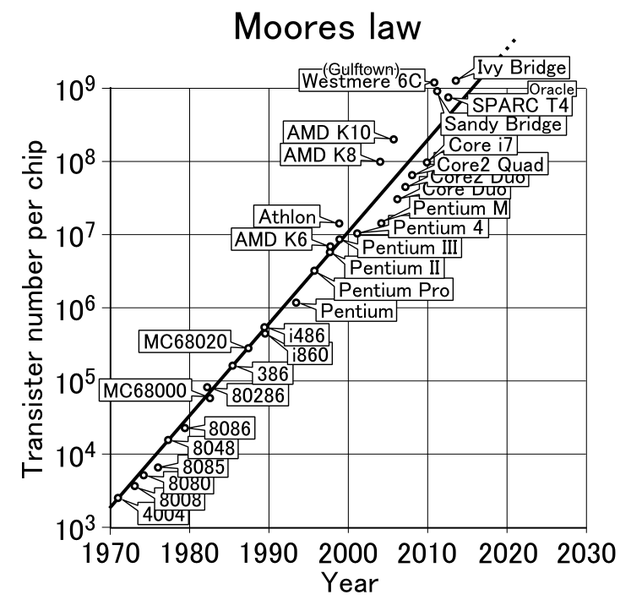
\includegraphics[width=0.75\linewidth]{mooreslaw.png}
\end{center}
\vspace{-0.5cm}
\caption{Moore's law \cite{mooreslawpic}}
\label{fig:mooreslaw}
\end{figure}

The improvements of 2D architectures are primarily driven by the reduction of the transistor size. By reducing transistor dimensions, the switching speed is increased thanks to the shorter distance between the source and the drain, implying an improvement of the overall speed of the designs.

However, as the transistor size is decreasing, the observed improvement is also getting smaller. Indeed, a smaller transistor allows higher device density but will slightly decrease the dynamic and increase the total delay (sum of gate and interconnection delays) at the level of the complete circuit. Also, power consumption is increased due to higher leakage and increasing interconnection wire length \cite{5227192}. In Figure \ref{fig:delaygateinterconnect} is shown the trends in transistor gate delay and interconnect delay with IC fabrication technology where the crossover point represents the interconnect bottleneck \cite{kirchain2007}.

\begin{figure}
\begin{center}
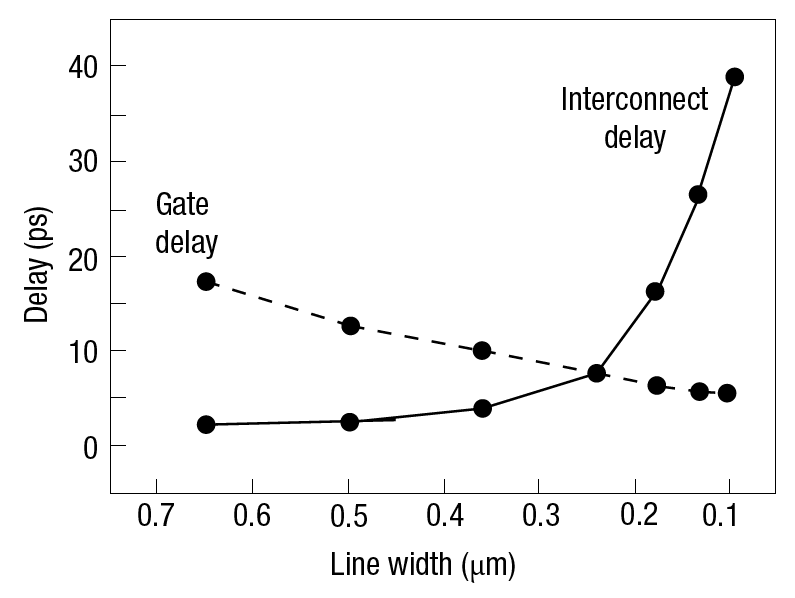
\includegraphics[width=0.75\linewidth]{delaygateinterconnect}
\end{center}
\caption{Trends in transistor gate delay and interconnect delay with IC fabrication technology \cite{kirchain2007}}
\label{fig:delaygateinterconnect}
\end{figure}

With the miniaturization, quantum effects such as quantum tunnelling will significantly affect how a transistor behave \cite{1240081}.

In addition to these physical aspects, economical considerations that will hinder the IC evolution beyond 20nm have to be taken into account \cite{5227192,PFF10}.

In order to overcome these limitations, new technologies have been proposed such as the carbon nanotubes \cite{tans1998room}, the nanowire transistors \cite{doi:10.1021/nl025875l}, the single-electron transistors \cite{citeulike:4194929}, but also the 3D-Stacked Integrated Circuits (3D-SIC) proposed by the academic and industrial communities. The latter has been often cited as the most prominent one~\cite{659500}.

Fast evolution of IC manufacturing technologies makes even the design of 2D-ICs a complex and tedious task with the growing number of design choices at the system level (e.g. number and type of functional units and memories, type and topology of the interconnection system, etc.) and physical level (respecting area/timing/power constraints). Using 3D-SICs introduces even more degrees of freedom: number of tiers, choices for manufacturing technology (e.g. full 3D integration, silicon interposer, face-to-face, back-to-face, etc.), 3D partitioning and placement strategies etc. These new degrees of freedom will contribute to the combinatorial explosion of already huge design spaces. Moreover, practice and 2D design experience cannot be fully exploited with 3D technology, since 3D-SICs change considerably the way ICs are implemented. The current design flows, which already showed their limits with conventional 2D-ICs, may thus need improvements to be able to deal with the increased complexity of emerging 3D-SICs \cite{vanderbiest06, PFF10}.

One of the solutions to face this problem is to develop high-level tools which can quickly explore design spaces and give early and reasonably accurate performance estimations based on physical prototyping of the 3D circuits~\cite{PFF10}.

In addition, performance estimation/optimization and the selection of the most-suitable solutions usually implies to take several objectives into account (e.g. maximization of the performance, minimization of the cost, minimization of the package size, etc.).

Currently, the design tools can be considered to follow a uni-criterion paradigm. Indeed, they have sequential development steps and each criterion is optimized without considering the impact on other criteria. This can lead to several rollbacks in the design flow since the achievement of the requirements can be time consuming (typical design iterations are measured in weeks).

On the other hand, multi-criteria approaches have been developed to optimize all the criteria simultaneously. Designing 3D-SICs inherently implies a huge design space and numerous degrees of freedom and criteria. This is the reason why we propose to apply this paradigm for the design of 3D-SICs.

\section*{Research questions}
Multi-objective optimization and multi-criteria decision aid were developed from the need of taking into account several criteria simultaneously. These tools from the operations research field have shown their abilities in solving similar problems in other fields, which also have a large solution space and applying metaheuristics have shown interesting results~\cite{talbi09}.

In this thesis, we will show the applicability of a multi-criteria paradigm for the design of 3D-SICs:
\begin{itemize}
\item how a 3D circuit can be modelled to apply multi-objective optimization
\item what kind of information can be provided to a designer
\item how multi-criteria decision aid can exploit these results to assist a designer
\end{itemize}

\section*{Outline}
In the first chapter, we will take an overview of the design and manufacturing of 3D-SICs. We will explain the limitations of current design flows and present the developments that have been carried out to overcome these problems. We will discuss why they should be improved and introduce how a multi-criteria paradigm can be useful.

In the chapter two, we will present an overview of the main tools in the MCDA fields where some of the most-used methods will be presented.

In the third chapter, we will define the problem we tackle (the 3D floorplanning) with the considered criteria. We will then show how a 3D-SIC can be modelled in order to apply multi-objective optimization. Simulations will be run on a case study and show what kind of information can be provided to a designer. The methodology will then be validated with a realistic case study to show the added value of a multi-criteria paradigm compared to a uni-criterion approach.

In the chapter four, we will show the robustness of the methodology and the associated algorithms. We will use classical indicators of the fields to analyse the convergence and diversity properties.

In the fifth chapter, we will explain how the obtained results can be exploited using multi-criteria decision aid. We will discuss on how such a paradigm can be used for designing circuits and what needs to be done in order to integrate it to actual design flows.

Finally, we will conclude on the results of the thesis and express some possible perspectives.



%\Chapter{Review of the literature}{Part I: Microelectronics design}
\label{cha:rol.icdesign}

\begin{summary}
In this chapter, we present a short overview of the 3D-stacked integrated circuits that have been proposed by the industrial and academic communities to overcome 2D-IC's limitations. We show how 3D-SICs can be designed and manufactured and and explain why current design flows should be improved to deal these new challenges.
\end{summary}

\section{Introduction}
In this chapter we will present a short overview of the 3D-stacked integrated circuits: show how then can be manufactured, their advantages and drawbacks, the challenges when designing them. We will then discuss about the limitations of current design flows and why they should be improved in order to address the complexity of designing 3D-SICs.
%\section{2D architecture and its limitations}
%
%In order to continuously improve the performance of integrated circuits (IC), technologists deploy enormous efforts to produce IC manufacturing process that is compelling to follow the well-known Moore's Law (see Figure \ref{fig:mooreslaw}). This empirical law predicts a doubling of the transistors' integration each 18 months and therefore increasing logic capacity of the circuit per unit area. 
%
%\begin{figure}
%\begin{center}
%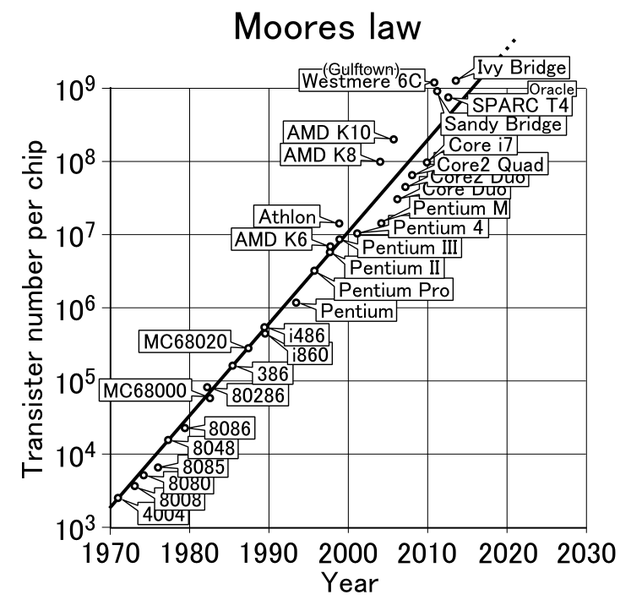
\includegraphics[width=0.75\linewidth]{mooreslaw.png}
%\end{center}
%\vspace{-0.5cm}
%\caption{Moore's law \cite{mooreslawpic}}
%\label{fig:mooreslaw}
%\end{figure}
%
%The improvements of 2D architectures are primarily driven by the reduction of the transistor size. By reducing transistor dimensions, the switching speed is increased thanks to the shorter distance between the source and the drain, implying an improvement of the overall speed of the designs.
%
%However, as the transistor size is decreasing, the observed improvement is also getting smaller. Indeed, a smaller transistor allows higher device density but will slightly decrease the dynamic and increase the total delay (sum of gate and interconnection delays) at the level of the complete circuit. Also, power consumption is increased due to higher leakage and increasing interconnection wire length \cite{5227192}. In Figure \ref{fig:delaygateinterconnect} is shown the trends in transistor gate delay and interconnect delay with IC fabrication technology where the crossover point represents the interconnect bottleneck \cite{kirchain2007}.
%
%\begin{figure}
%\begin{center}
%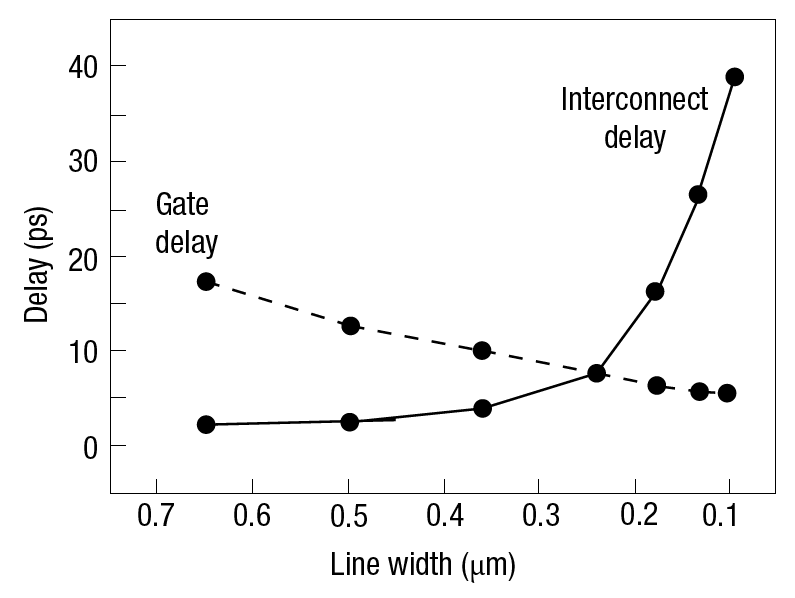
\includegraphics[width=0.75\linewidth]{delaygateinterconnect}
%\end{center}
%\caption{Trends in transistor gate delay and interconnect delay with IC fabrication technology \cite{kirchain2007}}
%\label{fig:delaygateinterconnect}
%\end{figure}
%
%With the miniaturization, quantum effects such as quantum tunnelling will significantly affect how a transistor behave \cite{1240081}.
%
%In addition to these physical aspects, economical considerations that will hinder the IC evolution beyond 20nm have to be taken into account \cite{5227192,PFF10}.
%
%In order to overcome these limitations, new technologies have been proposed such as the carbon nanotubes \cite{tans1998room}, the nanowire transistors \cite{doi:10.1021/nl025875l}, the single-electron transistors \cite{citeulike:4194929}, but also the 3D-Stacked Integrated Circuits (3D-SIC) proposed by the academic and industrial communities. The latter has been often cited as the most prominent one~\cite{659500}.

\section{3D integration}

Most of the current ICs are designed with electronic components (i.e. transistors) that are planar (although multi-gate transistors, such as finFETs tends to extend in the 3rd dimension) interconnected using up to a maximum of 12 (also planar) wiring (metal) layers per circuit. Those conventional ICs can thus be considered to be two-dimensional (2D)-ICs since both device and interconnect are predominantly made in a planar way \cite{1393404,fujitsu08}. As a major evolution of 2D-ICs, 3D-SICs are designed with multiple traditional 2D-ICs (that are manufactured independently, using standard CMOS technology) that are assembled (stacked) vertically in 3D-tiers. In face to back configuration, different 2D circuits communicate between tiers using vertical interconnections that need to connect front side of the chip and the backside, i.e. they need to traverse bulk silicon. These connections can be Through Silicon Vias (TSV) and if a face to face configuration is used micro bumps (µBump) or copper pads (CuPad) can also be used. They can be today manufactured with satisfactory geometrical properties, namely their diameter, pitch and height, allowing efficient integration of real-world systems~\cite{1705326,5746413}. This is shown in Figure~\ref{fig:3D_SIC_SOC2010}, where 2 dies, oriented face down are connected. An active component (i.e. logic gate) of the T1 is connected to the T2 using a TSV, back side metallization layer (to enable TSV placement anywhere in the T1 die), and µbump on the top layer of the T2, that is then connected, through a series of metal layers of the T2, to the active component of the top tier (T2).

\begin{figure}[h!]
\begin{center}
%\includegraphics[width=1\linewidth]{3D_SIC_SOC2010.png}
\includegraphics[width=0.5\linewidth]{3DSIC.pdf}
\end{center}
\vspace{-0.5cm}
\caption{Illustration of the wiring properties of a 3D-SIC}
\label{fig:3D_SIC_SOC2010}
\end{figure}

%The benefits of using 3D-ICs are numerous and have been already pointed out in the literature very often over the past few years \cite{659500}. These advantages will be summarized in the next subsections.
%First, by adding vertical dimension to the construction of the physical IC we can increase the IC packaging density. This means more gates for the same circuit footprint, that is much higher functional complexity of the final circuit for the same packaging volume. Secondly, the 3D-SICs are expected to have much better computing/power dissipation ratio. The integration in the 3rd dimension allows the design of circuits with different parts being closer to each other, resulting in less and shorter wires \cite{981091}. Lowering wire delays and allowing higher operating frequencies will result in increased bandwidths between nodes satisfying data hungry applications. Also, less and shorter wires mean lower total parasitic capacitance and inductance of the circuit, resulting in lower power dissipation. Finally, the 3D-SICs will enable the design of really heterogeneous systems, embedding not only traditional digital circuits such as processors and memories, but also analogue circuits such as sensors, antennas and power supplies \cite{4299568}.

%Currently different technologies for fabrication of 3D-SICs have been proposed in the literature. Proposed methods have been used for implementation of complete systems going far beyond simple proof-of-concept or feasibility demonstrators. One can mention the implementation of a processor and memory in a single 3D chip dedicated for video coding applications \cite{1696226} and a processor with multiple levels of memory hierarchy dedicated for high-throughput server applications \cite{1168873}. Finally, the first commercial 3D-SIC products have been already announced by IBM \cite{1167715} and companies specialized in 3D semiconductor industry such as Tezzaron \cite{terra04}.

%3D Integration is taken into account in the roadmaps of almost all key players in the field of integrated circuit design and manufacturing.

\subsection{Manufacturing technologies}

Several 3D manufacturing technologies have been proposed and have been used to implement complete systems. Among the existing possibilities, four major categories of methods that illustrate 3D integration can be cited \cite{659500,1652906}.

\paragraph{Transistor stacking}

The transistor stacking consists in creating several transistors level on one substrate. This should be the better way to manufacture 3D circuits although the success rate are currently limited due to thermal issues among the different limitations. The required temperatures to create a layer of high-performance transistors would provoke the destruction of the copper and aluminium already laid down on the previous layer \cite{659500}.

\paragraph{Chip stacking}

This methods consists in stacking components that have been designed and tested separately to produce a system-in-package (SiP). The vertically-stacked chips are interconnected with traditional wirings (lateral wire bondings). The principal advantage of this method is an improvement in terms of size. The wirings are shorter however the components integration density is not increased compared to a 2D system.

\paragraph{Die-on-wafer stacking}

In this method, known good dies (KGD), which are functional tested chips, are connected to a host wafer containing other KGDs. These KGDs can be interconnected with organic glues, oxide or metal bonding. The wafer and the bonded KGDs are then shaped to create the interconnections. Different substrates can be combined if the required temperature is low enough to minimize non-homogeneous expansion effects.

The die-on-wafer stacking can use interconnections on the edges of the chips or through-die. Depending on the interconnection type, this method can produce a better integration level than the chip stacking, with a better cost per connection ratio and a higher interconnection density, while holding the advantages of the KGDs.

The quality of the stacking depends on the pick-and-place equipment which is used to position the dies on the wafer. The placement accuracy will determine the possible interconnection density. Also, current equipments are supposed to handle fully buffered chips, not naked circuits so it does not provide protection to static discharge. 

\paragraph{Wafer-level stacking}

This methods consists in bonding entire wafers into a stack. The vertical through-wafer connections are made directly trough each substrate to the next wafer and it transistors layer. Similarly to the previous method, the interconnection density rely on the precision of the alignment, which is however currently better than the die-on-wafer stacking. This greater accuracy implies a better cost per connection ratio and a higher interconnection density compared to the die-on-wafer stacking.

The use of mixed substrates is also possible, only limited by the process temperatures. All the processing is done at the wafer level so wafer handling equipments are used. Since these provide protection to static discharge so there is no need to include buffering between the layers. The methods to bind two wafers are the same that are available for the die-on-wafer method.

One drawback to wafer-level stacking is its efficiency, since the chips on a wafer are not all KGDs.

\subsection{3D-SIC advantages}

\paragraph{Interconnection length}

The 3D integration allows to design circuits with components closer to each other. Wire of a few millimetres long can be replaced by TSV of a few tens of microns, as shown in Figure \ref{fig:wire}. These shorter interconnections will introduce shorter delays, hence allowing higher working frequencies \cite{659500,981091}.

\begin{figure}[h!]
\begin{center}
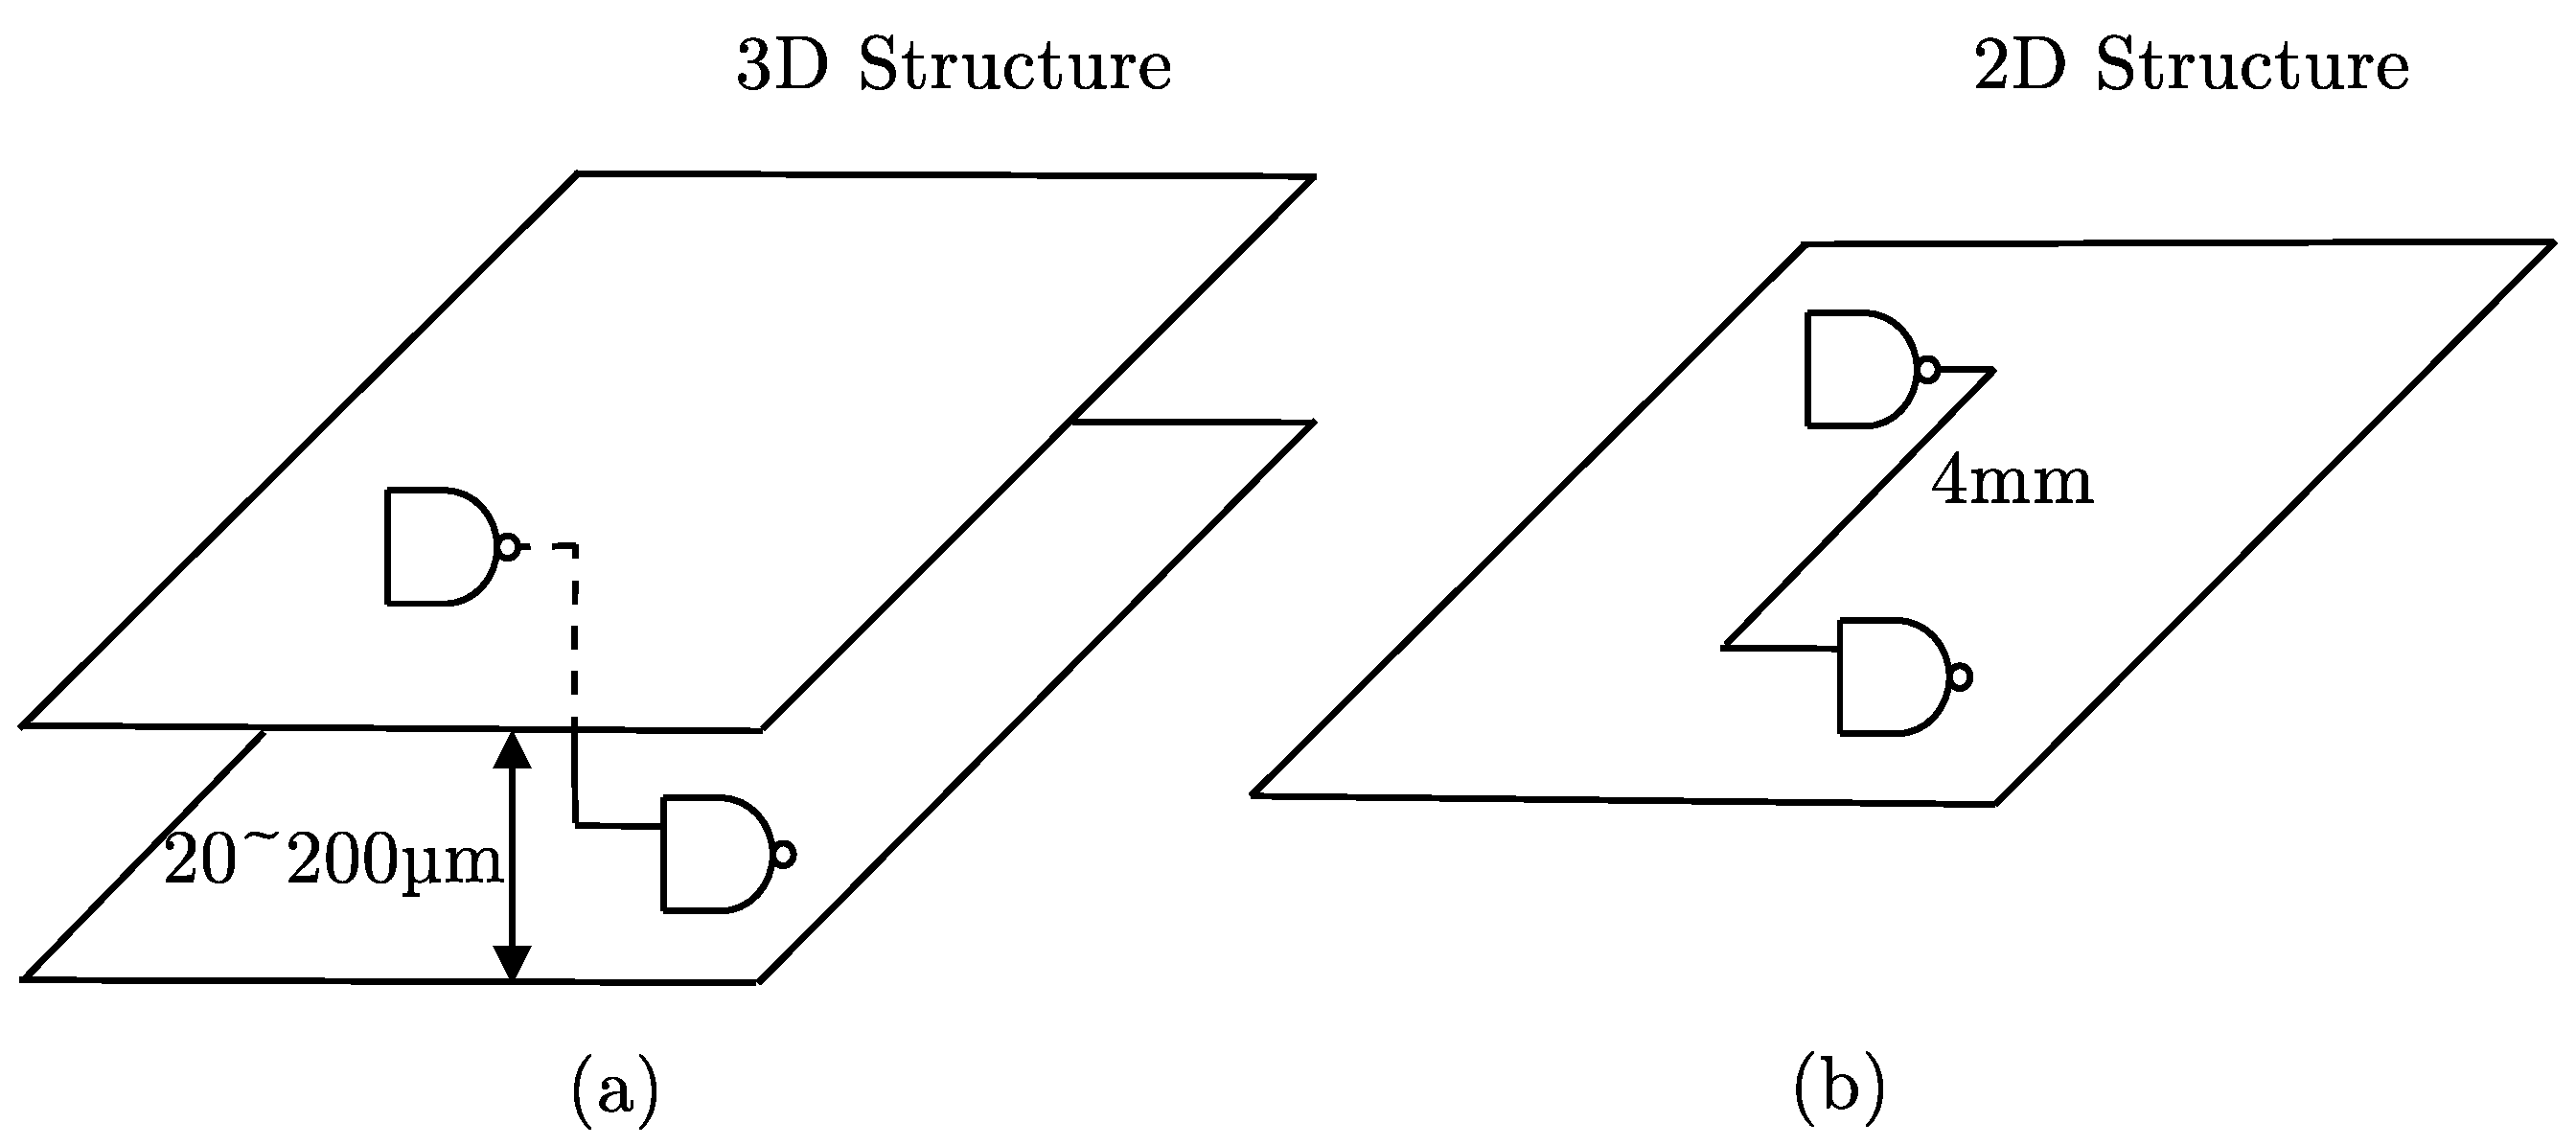
\includegraphics[width=0.8\linewidth]{wire.eps}
\end{center}
\vspace{-0.5cm}
\caption{Shorter interconnections \cite{659500}}
\label{fig:wire}
\end{figure}

\paragraph{Silicon efficiency and accessibility}

Adding a vertical dimension allows to increase the integration density. It is therefore possible to have more logic gates than a 2D-IC for the same footprint, hence a more efficient use of the silicon as shown in Figure \ref{fig:footprint}. For instance, compared to the footprint of a 2D-IC, the 3D-SICs can double the integration for a 50\% use of a 2D footprint \cite{659500}.

\begin{figure}[h!]
\begin{center}
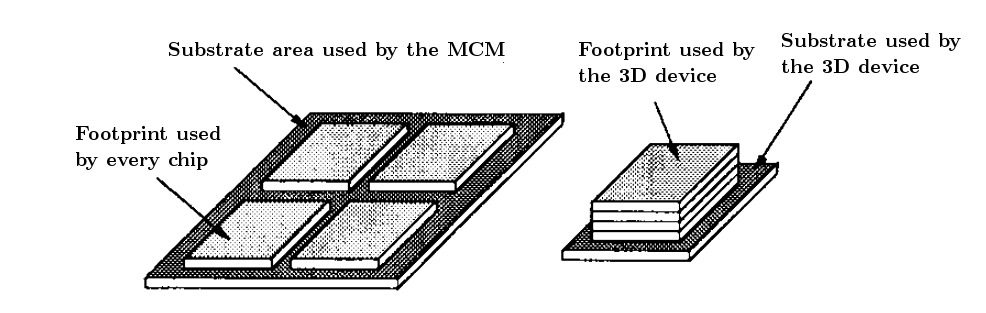
\includegraphics[width=0.8\linewidth]{footprint.png}
\end{center}
\vspace{-0.5cm}
\caption{Silicon efficiency \cite{659500}}
\label{fig:footprint}
\end{figure}

In addition, the 3D integration allows a better accessibility for the components, as shown in Figure \ref{fig:accessibility}. Indeed, for a 2D structure, 8 accessible neighbours can be considered for a central element (Figure \ref{fig:accessibility} (a)), whereas for a 3D structure, the number of accessible neighbours can reach 116 with through-tiers interconnections (Figure \ref{fig:accessibility} (b)) \cite{659500}.

\begin{figure}[h!]
\begin{center}
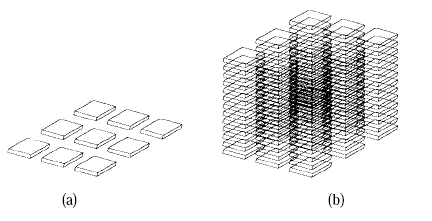
\includegraphics[width=0.8\linewidth]{accessibility.png}
\end{center}
\vspace{-0.5cm}
\caption{Components accessibility \cite{659500}}
\label{fig:accessibility}
\end{figure}

\paragraph{Bandwidth}

The use of TSVs on 3D-SIC can significantly increase the bandwidth of a circuit. Indeed, as shown in Figure \ref{fig:bandwidth}, the interconnections are not only limited to peripheral connections but can also make use of the circuit's surface. At a same working frequencies, this allows more bandwidth while at lower frequencies, the same bandwidth usage will require less power.

\begin{figure}[h!]
\begin{center}
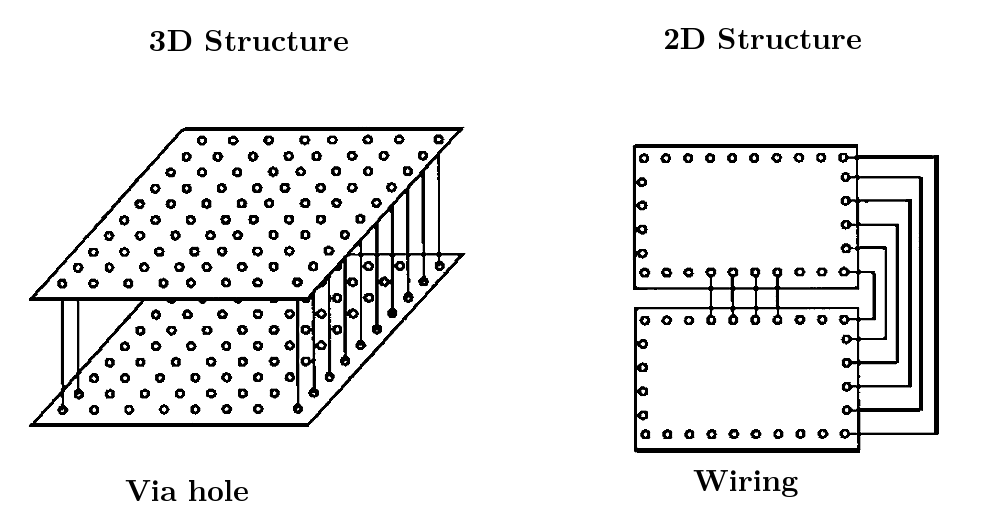
\includegraphics[width=0.75\linewidth]{bandwidth.png}
\end{center}
\vspace{-0.5cm}
\caption{Bandwidth improvement \cite{659500}}
\label{fig:bandwidth}
\end{figure}

\paragraph{Consumption and noise}

Shorter interconnections generally translates into lower capacitance and inductance parasitics. This means a decrease of the numbers of repeaters, hence a better consumption, less noise and less jittern hence lower delays and power consumption.

\paragraph{Heterogeneous circuits}

The 3D technologies allow truly heterogeneous designs. For instance, it is possible to integrate, in addition to traditional digital circuits of different technologies, analogical circuits such as sensors or antennas, as well as power supply, which give 3D-SIC a high degree diversity. It is also possible to mix old and new generations technologies to lower the cost of future circuits.\cite{4299568}.
%The Fig. \ref{fig:heterogeneity} shows a schematic view of a 3D-SIC developed by IMEC for biomedical purposes that contains antennas, DSPs, EEG/ECG sensors, a power supply and solar cells \cite{4198870}.

%\begin{figure}[h!]
%\begin{center}
%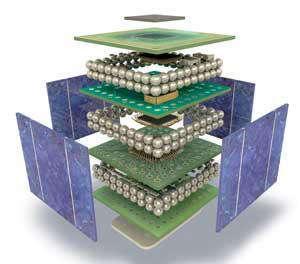
\includegraphics[width=0.5\linewidth]{heterogeneity.png}
%\end{center}
%\vspace{-0.5cm}
%\caption{Schematic illustration of an heterogeneous 3D-SIC (developed by IMEC) \cite{4198870}}
%\label{fig:heterogeneity}
%\end{figure}

\subsection{3D-SIC design challenges}

As explained, 3D-SICs offer numerous design perspectives thanks to their advantages. However there are drawbacks that need to be taken into account and that will be discussed in the following paragraphs.

\paragraph{Thermal dissipation}
The power density has increased exponentially over the past decades for the 2D-ICs and it appears that this trend will continue in the near future. As for 3D-SICs, due to their higher component density, they will also be subject to higher power density so thermal management should be considered carefully \cite{659500}. A simplified model of thermal dissipation has been developed in this thesis and will presented in Chapter \ref{cha:model}.

\paragraph{Cost}
With the appearance of a new technology, the involvement of a high cost should often be expected. In the case of 3D technology, in addition of the cost of the technology itself, there are the lack of infrastructure and the reluctance of manufacturers who do not want to risk to change to new technologies \cite{659500}.

\paragraph{Design complexity and design software}
A large number of systems have been implemented using the 2D technologies which means that current tools can cope with 2D design complexity even if they show more and more their limits \cite{vanderbiest06, PFF10}. As for 3D-SICs, the increased complexity can be tackled by developing adapted software \cite{659500}. However, to the best of our knowledge, few 3D dedicated software currently exist. One can nevertheless cite the works in \cite{1112292,1594713,Xie:2006:DSE:1148015.1148016,4735042}. Most of other tools are mainly developed for and owned by particular manufacturers. In addition, they are based on 2D design tools which does not allow to tackle the complexity of 3D designs integrally as they do not take all 3D specificities into account. For example, as it will be shown in Section \ref{sec:currentflows}, 3D partitioning and floorplanning are considered separately (as it is done for 2D-ICs) whereas the 3D geometrical assignment should be taken as a whole.

In the following section, we will have an overview about these software tools and generally about the design flow used to design integrated circuits.

%\section{2.5D-ICs by Xilinx}
%Now that the 3D integration has been introduced, let us give some notes that are worth mentioning about the 2.5D-ICs introduced by Xilinx \cite{bolsens2011}. 2.5D integration can be considered as a stepping stone to 3D design, as illustrated in Figure \ref{fig:2d5xilinx}. This technology is based on a silicon interposer where are placed the dies. The bindings required to connect the dies are located on this silicon interposer, as shown in Figure \ref{fig:siliconinterposer}. Compared to classical 2D-ICs, this allow higher interconnect density while being less challenging than 3D-SICs in terms of design flow, thermal issues, reliability, testing and cost as the technology is already existing.
%
%\begin{figure}[h!]
%\begin{center}
%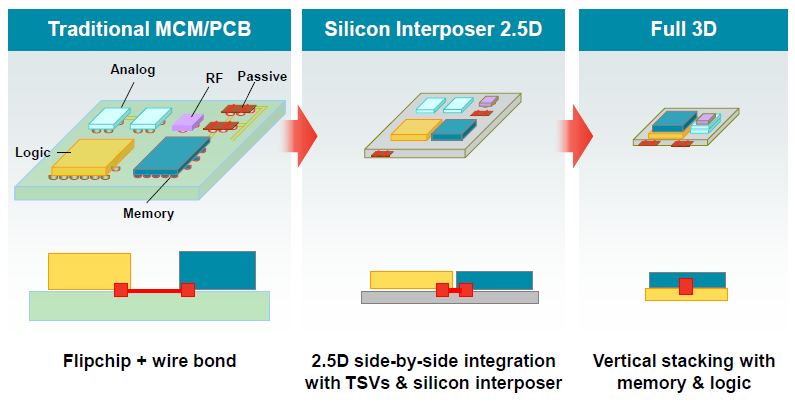
\includegraphics[width=0.8\linewidth]{2d5xilinx}
%\end{center}
%\caption{2.5D as a stepping stone to 3D integration \cite{bolsens2011}}
%\label{fig:2d5xilinx}
%\end{figure}
%
%\begin{figure}[h!]
%\begin{center}
%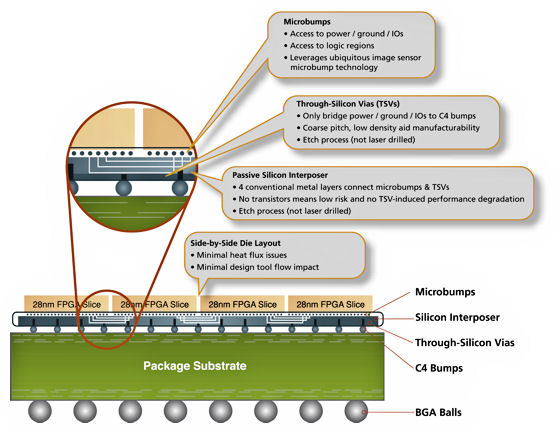
\includegraphics[width=0.8\linewidth]{siliconinterposer}
%\end{center}
%\caption{Illustration of the 2.5D integration with a silicon interposer \cite{bolsens2011}}
%\label{fig:siliconinterposer}
%\end{figure}
%
%In the following section, we will have an overview about these software tools and generally about the design flows used to design integrated circuits.

\section{Current design flows and their limitations}
\label{sec:currentflows}

Design flows are the combination of electronic design automation (EDA) tools used to produce an integrated circuit. These flows can generally be summarized in 4 main steps \cite{coursefred}, as shown in Figure \ref{fig:designflow}.

\begin{figure}[h!]
\begin{center}
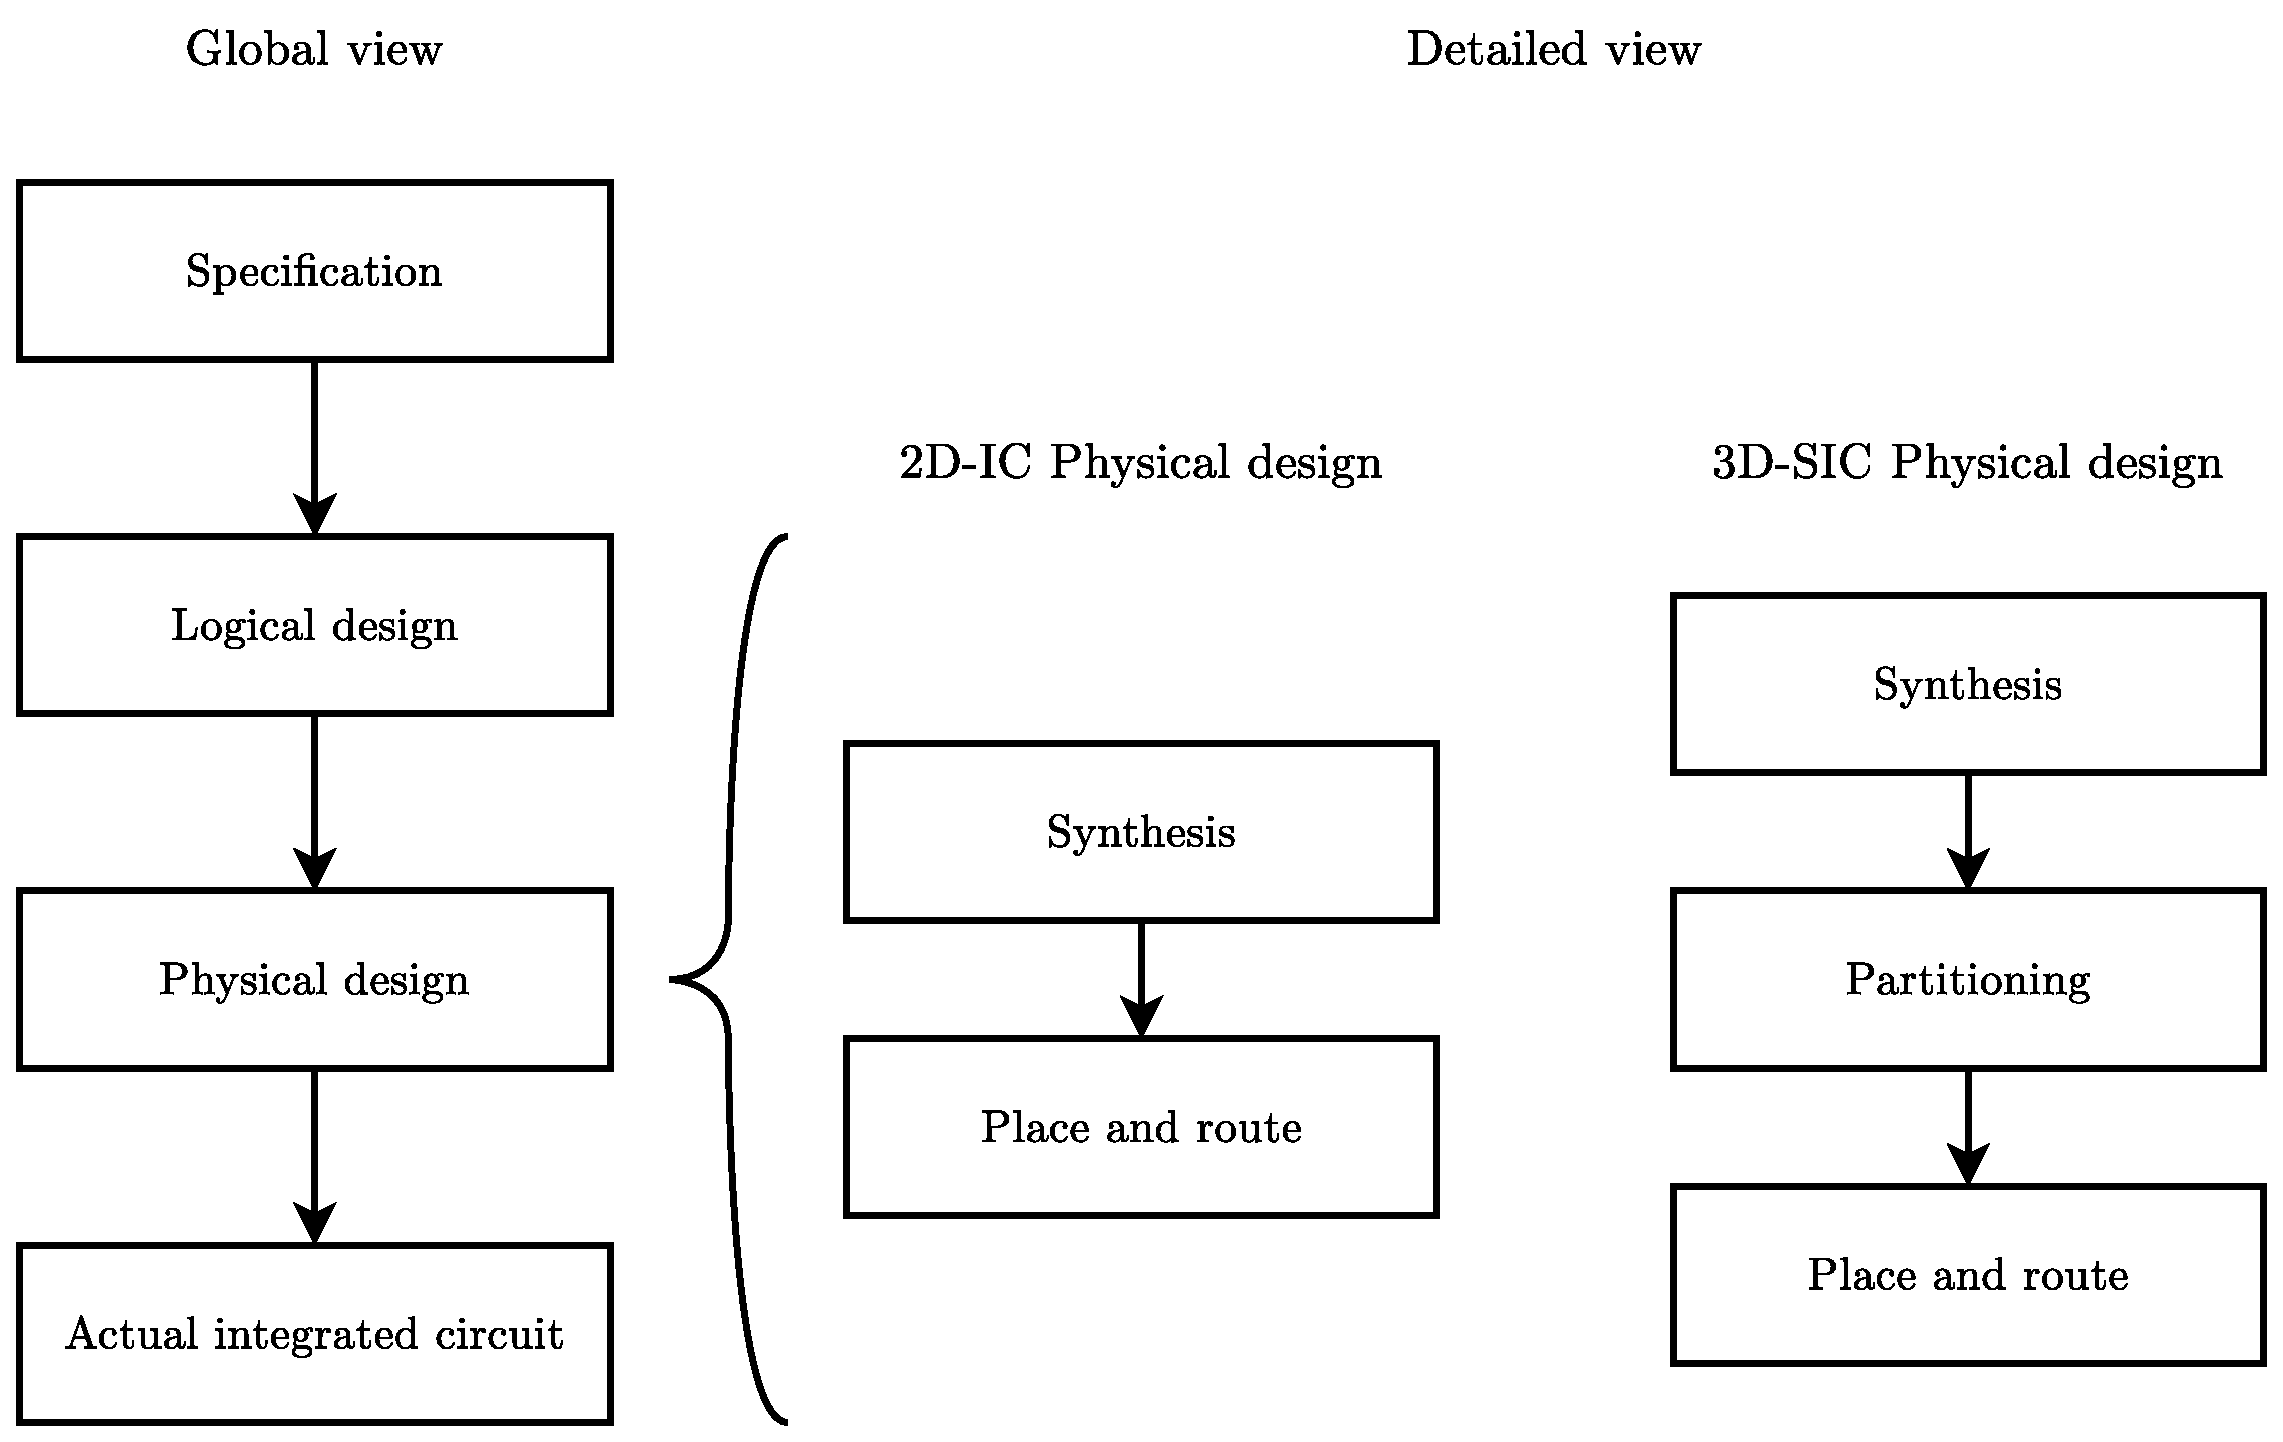
\includegraphics[width=\linewidth]{designflow2.eps}
\end{center}
\vspace{-0.5cm}
\caption{Classical design flow}
\label{fig:designflow}
\end{figure}

As one can observe, the design flows are sequential. The process goes from one step to the other with local optimization loops. In practice, it is not unusual to have several rollbacks to the previous steps due to the need of manual intervention to adjust the constraints and reach good solutions. %For instance, the optimization done in the logical design step might work in simulations but can be impractical for the physical design step so a rollback is needed in order to correct this inconsistency.

As explained previously, designing ICs implies numerous choices. At the moment, with this growing complexity, the current design flows can already show their limits. Indeed, these tools are developed to only take into account particular specificities of a circuit (area, timing) whereas other characteristics also have to be optimized. Besides, most of the time, the designers will be likely to freeze a certain amount of choices on basis of their experience, and then begin the optimization process with the remaining parameters. This will therefore limit the exploration of the design space and other good solutions may be ignored. In addition, the fixed choices can be questionable since they are based on the designer's experience and it is difficult to master the whole complexity of the problem in terms of criteria and possibilities of design.

The current design flows, which already showed their limits with conventional 2D-ICs, may thus need improvements to be able to deal with the increased complexity of emerging 3D-SICs \cite{vanderbiest06, PFF10}.

For the moment, most 3D design flows adapt classical flows to include 3D specificities, in particular 3D partitioning and 3D place \& route (see Figure \ref{fig:designflow}). We can observe that these two steps are separated: the circuits are first (manually) partitioned, then the place \& route occurs for each layer. However, one can guess that the performances of a 3D-SIC will depend on the position of a component, considering simultaneously its position on a layer ((X,Y)-coordinates) and the layer where it lies (Z-coordinate). 3D design flows therefore need improvements to take into account these three coordinates at the same time.

\section{Design space exploration tools}

In order to cope with the increasing complexity of integrated circuits and the limitations of the current design flows, numerous tools have been proposed, in particular works about design space exploration (DSE) that have been developed to quickly suggest possible interesting solutions to a designer and speed up the design processes. In this section, we will describe different DSE tools that have been proposed in the literature.

\subsection{2D-IC tools}

\paragraph{MILAN}

The MILAN (Model based Integrated simuLAtioN) framework \cite{Mohanty02rapidsystem-level} aims to simplify the optimization and the exploration of design spaces for System-on-Chip (SoC) platforms. This tool works on the component level and allows the users to choose a compromise between the simulation speed and the results accuracy. The exploration and optimization process is done in two phases: first it searches for possible combinations between the architecture, the application and the mapping and second it estimates the performances (power, latency) depending the precision asked by the users.

\paragraph{SoC Architecture Explorer}

SoC Architecture Explorer \cite{ueda05architecture} is a multi-objective optimization and exploration tool that aims the design of SoC architectures by evaluating the compromises between the footprint and the execution time. The exploration process focuses on the application and the system architecture where the tool analyses the data flow and estimates the data transfers to determine a number of possible architectures.

%http://www.esteco.com/index.jsp
\paragraph{modeFRONTIER (ESTECO)}

modeFRONTIER \cite{esteco01} is a proprietary development environment developed by ESTECO. It is a multi-objective optimization tool that aims parallel SoC architectures. modeFRONTIER allows to deal with up to one million different design configurations thanks to statistical analysis tools and data mining techniques.

%http://www.multicube.eu/
\paragraph{MULTICUBE}

The MULTICUBE project (MULTI$^{3}$) \cite{multicube08, Silvanoetal09} is a European project started in 2008 and dedicated to the multi-objective exploration of MPSoC architectures for multimedia embedded systems. The aims is to developed a framework that allows a quick and automated exploration of the design space to improve the performances of a MPSoC with metrics such as power, latency, computing performance, bandwidth, QoS, etc. This project is based on several heuristics and optimization algorithms that reduce the exploration time and allow a quick selection of the best solutions. In addition, MULTICUBE also aims to define an application-oriented framework based on the results of the multi-objective exploration to optimize the resources allocation and the tasks scheduling of the applications. The exploration is done at the system level, using the SystemC language. The project includes proprietary and open-source tools whose development targets the industry. Among the developed prototyping tools, Multicube explorer and Multicube-SCoPE can be cited.

%http://home.dei.polimi.it/zaccaria/multicube_explorer_v1/Home.html
\subparagraph{Multicube Explorer}

Multicube Explorer \cite{m3explorer09} is a design space exploration framework for supporting platform-based design. This tool allows a fast optimization of a system with objective functions such as power, delays, surface, etc. by means of a system simulator. Multicube explorer proposes several multi-objective optimization methods that aim to propose the best compromises.

%http://www.teisa.unican.es/gim/en/scope/multicube.html
\subparagraph{Multicube-SCoPE}

Multicube-SCoPE \cite{m3scope09} is an evolution of the SCoPE tool \cite{scope04} oriented to design space exploration. It is a fast system performance and power simulator providing metrics associated with a system in order to drive the DSE process.

\subsection{3D-SIC tools}

\paragraph{DSE for 3D-stacked DRAMs by Weis \textit{et al.}}
Design space exploration for 3D-stacked DRAMs has been developed by Weis \textit{et al.} \cite{5763068}. They defined a 3D-DRAM based on a SystemC model with a 3D channel controller and also considered a wiring model for the TSVs. The used metrics are area, performance and energy efficiency evaluated for different DRAM architectures and technologies. 3D thermal issues has been kept out of the scope of the study. The simulation results allowed them to have a trade-off analysis of horizontal wirings against vertical wirings in terms of energy and cell efficiency. They could show quantitatively how a 3D-DRAM can perform better than a classical DRAM.

\subparagraph{Observation}
This work is really interesting as it shows the stakes of using the 3D technology for DRAM. However, since it is based on DRAMs, the tools work with a memory structure that is repeated in the 3D-DRAM, which does not take into consideration more heterogeneous architectures. Also, only trade-off analyses are performed, which does not give a more global multi-criteria insight of the results as it will be illustrated in Chapter \ref{cha:rol.mcda}.

\paragraph{DSE for 3D architecture and DSE for 3D integrated circuits by Xie \textit{et al.}}
Design space exploration for 3D architecture and design space exploration for 3D integrated circuits are two works proposed by Xie \textit{et al.} \cite{Xie:2006:DSE:1148015.1148016,4735042}. In the first study, they combine several tools to perform a DSE:
\begin{itemize}
\item for the 3D cache partitioning, two strategies have been proposed at the subarrays granularity level
\item the area, the delay and the energy of a 3D cache are assessed following a cost function
\item 3DCacti, a tool developed to explore various 3D partitioning options of caches
\item thermal-aware 3D floorplanning based on simulated annealing
\end{itemize}
With the DSE, they are able to propose different possible architectures for 3D microprocessor design by performing trade-off analyses of the criteria.
The second study is an extension where a cost analysis is added.
 
\subparagraph{Observation}
These works seem to be among the most integrated study in the literature with cache partitioning and microprocessor floorplanning, and considering several criteria including thermal issues. However, the partitioning and the floorplanning are separated while a more 3D approach should consider both dimensions simultaneously. Also, the criteria are aggregated with a cost function which can lead to inconsistency as it will be explained in Chapter \ref{cha:rol.mcda} and only trade-off analyses are performed.

\paragraph{Automated design flow for 3D microarchitecture evaluation by Cong \textit{et al.}}
An automated design flow for 3D microarchitecture evaluation has been proposed by Cong \textit{et al.} \cite{1594713}. They propose an evaluation flow for performance assessment and thermal management. This allows them to perform thermal-aware 3D floorplanning.

\subparagraph{Observation}
This work is worth mentioning as it proposes a quick way to evaluate temperature issues. However, it only deals with the thermal criterion.

\paragraph{PathFinding flow}
The PathFinding flow is a project proposed by IMEC and Atrenta \cite{5335663,DBLP:conf/3dic/MilojevicCCRRSAPM09} to deal with design exploration of advanced packaging integration. The aim of this work is to be able to produce a specification for the architecture and for the technology with assessment of performance, power and cost. The methodology is divided in 3 steps:
\begin{enumerate}
\item 3D system level design exploration with a rough estimation of the performance, power and cost parameters. The designer will be able to focus on the 2D design issues while manually considering the 3D specificities.
\item RTL (Register Transfer Level) elaboration, which links the system level to the physical design by producing RTL models.
\item 3D physical design prototyping, which allows fast exploration of the physical design impact of alternative design/technology options on the performance, power and cost parameters.
\end{enumerate}

\subparagraph{Observation}
This work is also among the most integrated study in the literature. However, the criteria optimization is done following a uni-criterion approach which does not allow to explore quickly several possibilities.

\section{Conclusion}
In this chapter, we have presented an overview of the evolution of IC design. Manufacturers have pushed back the limitations of the silicon for the past decades and are now facing new challenges due mainly to quantum effects. 3D-SICs have been proposed to face these problems and we have shown a quick review of this promising technology.

With the 3D integration, design flows have evolved and integrate 3D partitioning and 3D place and route. However, these two steps are performed separately while they should be considered simultaneously as the circuits' performances will depend on the position of a component on a layer and the layer where it lies.

We have then presented researches that aim to deal with these challenges by making use of multi-objective optimization. To the best of our knowledge, all these tools use a uni-criterion approach or deal with a limited set of criteria while performing only trade-off analyses. The goal of this research is to show that a more multi-objective-oriented optimization could be more suitable to take into account the many aspects of a design and that a more globa multi-criteria analysis can provide more information.

In the next chapter, we will describe a short overview of the tools coming from the operations research that will allow to take into account multiple criteria simultaneously.

\Chapter{Review of the literature}{Part II: Operations research}
\label{cha:rol.mcda}

\begin{summary}
\lipsum[1]
\end{summary}

\section{Introduction}
\label{sec:rol2.intro}
In this chapter, we briefly present the basics of multi-objective optimization and multi-criteria decision aid, in order to justify our choice to use such a paradigm. As stated in Chapter \ref{cha:rol.icdesign}, the 3D integration can offer new perspectives but designing 3D-SICs includes two major distinctive features: multiple criteria and a huge number of possible solutions. When facing such problems, two main methods exist: the uni-criterion paradigm and the multi-criteria paradigm. For optimization problems, these paradigm will refer to the terminology mono-objective/multi-objective optimization while for decision aid, the terminology uni-criterion/multi-criteria will be used.

In the following, we will briefly describe each paradigm, showing some of the main approaches alongside illustrative examples. We will first present the uni-criterion methodology, show why it can be limited in our contect and explain why a multi-criteria paradigm can be more suitable.

\section{The uni-criterion paradigm}
\label{sec:rol2.unicrit_paradigm}

\subsection{Problem formulation}
An optimization problem can be formulated, without loss of generality, as \cite{BraMar2002}
\begin{equation}
\label{eqn:optiprob}
\begin{gathered}
\min f(x)\\
x \in A
\end{gathered}
\end{equation}
where $f$ is a real-valued function evaluating the solutions denoted $x$, and $A$ is the set of solutions, $f$ is also called the \emph{criterion} on which $x$ is evaluated. Let us note that the equation \ref{eqn:optiprob} expresses a \emph{minimization} problem. A \emph{maximization} problem can be seen as a minimization problem with the identity
$$
\max_{x \in A} f(x) = - \min_{x \in A} (-f(x))
$$
so that there is no loss of generality by using only \emph{minimization} formulation.

In order to give a more precise idea of what an optimization problem is, we will describe in the next section some typical examples taken from the reference book \cite{talbi09, BraMar2002}.

\subsection{Examples of typical optimization problems}
\subsubsection{Linear programming}
Linear programming (LP) is a problem formulation where the aim is to optimize a linear function, subject to linear inequality constraints. This can be formulated as follows:
\begin{equation}
\min \mathbf{c}^\intercal\mathbf{x}
\end{equation}
subject to
\begin{equation*}
\begin{gathered}
A\mathbf{x} \leq \mathbf{b}\\
\mathbf{x} \geq \mathbf{0}
\end{gathered}
\end{equation*}
where $\mathbf{x}$ is a vector of continuous, integer or boolean variables to be determined, $\mathbf{c}$ and $\mathbf{b}$ are vectors of coefficients, $A$ is a matrix of coefficients.

Efficient exact methods for solving LP problem exist such as, among the most knowns, the simplex algorithm \cite{dantzig51} or the interior point method \cite{Karmarkar84}.

\begin{example}[Linear programming]
A given company produces two electronic boards $Board_1$ and $Board_2$ based on two kinds of memories $M_1$ and $M_2$. The objective consists in finding the most profitable product mix, given the availability of each memory $M_1$ and $M_2$, and for each board $Board_i$ the used amount of memories and the profit, as shown in Table \ref{tab:ex_lp}. The decision variables are $x_1$ and $x_2$ that represent respectively the amount of $Board_1$ and $Board_2$. The objective is to maximize the profit.\\
The problem can be formulated as an LP:
\begin{equation*}
\text{max profit } = 5x_1 + 4x_2
\end{equation*}
subject to the constraints
\begin{eqnarray*}
192x_1 + 128 x_2 &\leq& 1024\\
32x_1 + 64_x2 &\leq& 192\\
x_1, x_2 &\geq& 0
\end{eqnarray*}
\end{example}

\begin{table}[h!]
\begin{center}
\caption{Data associated with the LP problem}
\begin{tabular}{|l|c|c|c|}
\hline
& Usage for $Board_1$ & Usage for $Board_2$ & Availability\\
\hline
$M_1$ & 192 & 128 & 1024 \\
$M_2$ & 32 & 64 & 192 \\
Profit per unit & \euro 5 & \euro 4 & \\
\hline
\end{tabular}
\label{tab:ex_lp}
\end{center}
\end{table}

\subsubsection{Integer linear programming}
Integer linear programming deals with linear problems where the variables are restricted to be integers:
\begin{equation}
\min \mathbf{c}^\intercal\mathbf{x}
\end{equation}
subject to
\begin{equation*}
\begin{gathered}
A\mathbf{x} \leq \mathbf{b}\\
\mathbf{x} \geq \mathbf{0}\\
\mathbf{x} \in \mathbb{N}
\end{gathered}
\end{equation*}
where $\mathbf{c}$ and $\mathbf{b}$ are vectors and $A$ is a matrix of coefficients.

When the decision variables are both discrete en continuous, the problem refers to \textbf{mixed integer programming} (MILP).

Other particular ILP problems which deals with variables that are restricted to be either 0 or 1 are called \textbf{0-1 linear programming}.

\begin{example}[Travelling salesman problem (TSP) \cite{talbi09}]
This is one of the most known optimization problem. It can be formulated as follows: given $n$ cities and the distance between each pair of cities, we have to find the shortest tour that visits each city once and returns to the origin city. This problem can be formulated as an ILP problem.\\
Let $d_{ij}$ be the distance between the city $i$ and the city $j$, $S$ be the set of solutions (tours) and define:
\begin{equation*}
x_{ij} = \left\{
	\begin{array}{l l}
	1 & \text{if the path goes from city $i$ to city $j$}\\
	0 & \text{otherwise}
	\end{array}
\right.
\end{equation*}
The ILP formulation is then:
\begin{equation*}
\min \sum\limits_{i=0}^{n} \sum\limits_{j=0, j \neq i}^{n} d_{ij} x_{ij}
\end{equation*}
s.t.
\begin{equation*}
\begin{array}{l l}
\sum\limits_{i=0, i \neq j}^{n} x_{ij} = 1 & \quad j = 0, \dots, n\\
\sum\limits_{j=0, j \neq i}^{n} x_{ij} = 1 & \quad i = 0, \dots, n\\
\sum\limits_{i \in S, j \notin S} x_{ij} \geq 1 & \quad \forall S \subset \{1, \dots, n\}\\
0 \leq x_{ij} \leq 1 & \quad \forall i,j\\
x_{ij} \in \mathbb{N} & \quad \forall i,j
\end{array}
\end{equation*}

\end{example}

\subsubsection{Non-linear programming}
Non-linear programming (NLP) models deal with mathematical problems where some of the constraints and/or the objective function are non linear:
\begin{equation}
\min f(x)
\end{equation}
where
\begin{equation*}
\begin{gathered}
f: \mathbb{R}^n \rightarrow \mathbb{R}\\
x \in \mathbb{R}^n
\end{gathered}
\end{equation*}
subject to
\begin{equation*}
\begin{gathered}
g_i(x) \leq 0, i \in J = 1, \dots, m
\end{gathered}
\end{equation*}
where $g_i : X \rightarrow \mathbb{R}^n$ are the inequality constraints.

NLP are generally more difficult to solve than LP \cite{talbi09} and metaheuristics (see Section \ref{subsec:metaheuristics}) are commonly used to solve this class of problems.
%\subsubsection{Dynamic programming}


%\subsubsection{Assignment problem}


\section{From the uni-criterion paradigm to the multi-criteria paradigm}
\label{sec:rol2.unicritmulticrit}

With a uni-criterion paradigm, the optimization of one criterion is generally performed while considering that this single criterion synthesizes all the characteristics of the problems or that the other criteria already satisfy an acceptable level. This methodology will try to give a solution which is supposed to be optimal according to this criterion. However, most problems encountered in the field of IC design, and more generally in other industrial fields, contains several conflicting criteria as it will be illustrated in Chapter \ref{cha:model}. Finding a solution that simultaneously optimizes all the criteria is only possible in rare cases and if optimality can be reached.
%, there may be cases where several solutions share the same evaluations on all the criteria.

For instance, when designing ICs, a manufacturer will try to simultaneously maximize the performance while minimize the cost of the circuit. However, we can already guess that those two objectives are conflicting. Also, producing high-end ICs can be subject to more difficulties in terms of thermal dissipation. In addition, a criterion based on ecological standards may have impacts on the cost and the performance of an IC.

This example shows that a uni-criterion approach cannot always be applied since there is no achievable optimum as several criteria have to be simultaneously taken into account. A solution that optimizes one criterion will likely to affect another.

In order to deal with the multiple criteria of a problem, another paradigm consists in taking into account all the criteria simultaneously. This is the aim of the multi-criteria paradigm which aim to:
\begin{enumerate}
\item find the solutions that are efficient on all the criteria simultaneously with the multi-objective optimization;
\item provide support to a decision maker facing several conflicting solutions with multi-criteria decision aid (MCDA) that allows to highlight such conflicts and therefore obtain a compromise with a transparent process.
\end{enumerate}

\section{The multi-criteria paradigm}
\label{sec:rol2.multicrit_paradigm}

% In order to deal with the multiple objectives of a problem, another approach consists in taking into account all the criteria simultaneously. This is the aim of multi-criteria decision aid which goal is to provide support to a decision maker facing several conflicting solutions. MCDA allows to highlight such conflicts and therefore obtain a compromise with a transparent process.

\subsection{Problem formulation}
A multi-criteria problem can be formulated without loss of generality as follows \cite{BraMar2002}:
\begin{equation}
\label{multicrit_formulation}
\begin{gathered}
\min \{f_1(x), f_2(x), \dots, f_m(x)\}\\
x \in \mathcal{A}
\end{gathered}
\end{equation}
where $\{f_1(x), f_2(x), \dots, f_m(x)\}$ is a set denoted $\mathcal{F}$ of $m$ evaluation criteria that needs to be minimized and $x$ is a solution of the set $\mathcal{A} = \{a_1, a_2, \dots, a_n\}$.

As explained in Section \ref{sec:rol2.unicritmulticrit}, an optimal solution can be impossible to find for a multi-criteria problem. However, compromise solutions can exist and in order to identify them, a dominance relation has been defined \cite{BraMar2002}:

\begin{definition}[Dominance]
A solution $a_1$ dominates a solution $a_2$ if:
\begin{itemize}
\item $a_1$ is as least as good as $a_2$ on all criteria;
\item $a_1$ is strictly better than $a_2$ on at least one criterion.
\end{itemize}
\end{definition}

From this dominance relation, it is then possible to filter the solutions in order to keep only the non-dominated ones. This set of \emph{efficient} solutions is called the Pareto frontier. Let us note that the \emph{efficient} solutions refer to the decision space while the Pareto frontier refers to the evaluation space.

Two approaches can be used to establish this set~\cite{Vin92}:
\begin{itemize}
\item \textit{Exact methods} which aims to compute the Pareto frontier directly~\cite{EhrgottGandibleuxbook02,steuer86a}.
\item \textit{Approximate methods} which are based on metaheuristics to quickly explore the solution space and approach as best as possible the Pareto optimal frontier\cite{talbi09}.
\end{itemize}
As explained in Chapter \ref{cha:rol.icdesign}, designing 3D-SICs includes a huge solution space to deal with in the optimization process. The solution (that is to say the most-suitable 3D-SIC architecture) is unknown and an exhaustive search would take a prohibitive time. Also, due to the nature of the criteria (discrete and continuous variables, linear and non-linear criteria) that will be defined in Chapter \ref{cha:model}, we have few hopes to be able to develop an exact method. For those reasons, approximate methods with metaheuristics for multi-objective optimization will be used. Let us also remind that the aim of this thesis is to show the applicability of a multi-criteria paradigm to the design of 3D circuits. Therefore developing exact methods has been kept out of the scope of this work.

\subsection{Metaheuristics for multi-objective optimization}
\label{subsec:metaheuristics}
Metaheuristics are a family of approximate optimization methods. They aim to provide "acceptable" solutions in reasonable time for solving complex problems \cite{talbi09}. As stated previously, the optimal solution of a multi-objective optimization problem (MOP) is not a single solution but a set of solutions defined as Pareto optimal solutions. The main goal is therefore to obtain this set.

In our study, due to the heterogeneous nature of the criteria, there are few hopes to find the exact Pareto optimal solutions. In such cases, metaheuristics are commonly used and the goal is then to find an approximation of this set. Two properties has to be respected in order to ensure good approximations: convergence to the Pareto optimal front and uniform diversity. The first property allows to have solutions that are closed to the Pareto set whereas the second property shows a good distribution around the Pareto front.

Numerous metaheuristics have been developed since the 50s. Among the most known, let us cite genetic algorithm \cite{holland1975adaptation}, scatter search \cite{Glover77}, simulated annealing \cite{KirkpatrickGelattVecchi83}, tabu search \cite{Glover86}, memetic algorithms \cite{moscato89on} and ant colony optimization \cite{Dor92a.phd}.

In this work, we will focus on genetic algorithms (GA) as they are quick to implement for a first approach and are suitable to heterogeneous variables problems. More details about other metaheuristics can be found in reference books such as \cite{talbi09,dreo06metaheuristics,8125462}.

\subsubsection{General description of genetic algorithms}
Genetic algorithms have been developed by Holland in the 1970s \cite{holland1975adaptation}. They are metaheuristics that reproduce the properties of a natural selection process as described by Charles Darwin. GAs are based on the principle of the improvement of the gene pool of a population over generations. GAs will mimic the natural evolution with techniques such as selection, crossover and mutation. In the following, we will briefly describe the general methodology of a GA without considering a multi-objective case since the key steps are similar. Afterwards, we will describe one of the most popular multi-objective genetic algorithms: NSGA-II (Non-dominated Sorting Genetic Algorithm).

Genetic algorithms rely on a population that is evolved toward better solutions or individuals. The evolution is an iterative process and starts usually with a randomly-generated solutions. At each iteration, every individual is evaluated to define its fitness. The fitter ones are more likely to be selected for genetic modifications (crossover and possibly mutation). The produced solutions constitutes the new generation that will be used for the next iteration. The algorithm is commonly terminated when a maximum number of generations has been produced or when a certain fitness level has been satisfied. The general pseudo-code for genetic algorithms is shown in Algorithm \ref{alg:ga}.

\begin{algorithm}[h!]
\caption{General pseudo-code for genetic algorithms}
\label{alg:ga}
CHOOSE initial population;\\
EVALUATE each individual's fitness;\\
\Repeat{TERMINATION CONDITION satisfied}{
	SELECT parents;\\
	CROSSOVER pairs of parents;\\
	MUTATE the resulting offspring;\\
	EVALUATE the new candidates;\\
	SELECT individuals for the next generation;
}
\end{algorithm}

\paragraph{Representation of a solution}
The representation or encoding of a solution is called a chromosome and depends on the problem. Several examples of problems show binary encodings however, in our study we will use a real-valued matrix that will be detailed in Chapter \ref{cha:model}. Nevertheless, without loss of generality, we will illustrate the principles of a genetic algorithm by using binary-coded solutions.

\paragraph{Initialization}
Initially many solutions are generated, usually randomly to form the initial population. Depending on the problem, the generation of the initial population can be guided (seeded) to areas where optimal solutions are likely to be found.

\paragraph{Selection}
The selection is a stochastic process usually planned so that the fitter solutions have a higher probability of being selected. This aims to ensure the convergence of the algorithm.

In particular, one can mention the roulette wheel selection method where the fitness level is used to associate a probability of selection to each candidate. If $f_i$ is the fitness of the individual $i$, its probability to be selected is $p_i = \frac{f_i}{\sum_{j=0}^{n}f_j}$ where $n$ is the number of individuals in the population.

\paragraph{Crossover}
Once a pair of individuals has been selected, they will be crossed-over. Typically, two children are created from each set of parents. One method of crossover (one-point crossover) will be explained here but other approaches exists \cite{}. A random crossover point will be selected on both parents. Beyond that point, the data will be swapped with the information of the other parent as show in Example \ref{ex:crossover}.

\begin{example}[Crossover example]
\label{ex:crossover}
Let us consider two individuals $x$ and $y$ of the population:
\begin{table}[h!]
\begin{center}
\begin{tabular}{cccccccccc}
$x$ & = & 0 & 1 & 1 & 0 & 1 & 1 & 0 & 0\\
$y$ & = & 1 & 1 & 0 & 0 & 1 & 0 & 1 & 0
\end{tabular}
\end{center}
\end{table}

\noindent
If the randomly-chosen crossover point is 2 then the obtained offspring is:
\begin{table}[h!]
\begin{center}
\begin{tabular}{cccc|cccccc}
$x'$ & = & 0 & 1 & 0 & 0 & 1 & 0 & 1 & 0\\
$y'$ & = & 1 & 1 & 1 & 0 & 1 & 1 & 0 & 0
\end{tabular}
\end{center}
\end{table}
\end{example}

\paragraph{Mutation}
Mutation is a genetic operation used to ensure diversity in the generated populations. It changes one or more information in the chromosome of an individual. This alteration depends on how the solution is encoded. If it is a bit string, the most common operation is to apply a bit flip (see Example \ref{ex:mutation}) while for float chromosomes, new values can be generated following user-defined rules (see detailed illustration in Chapter \ref{cha:model}).

\begin{example}[Mutation example]
\label{ex:mutation}
Let us consider one individual $x'$ of the population:
\begin{table}[h!]
\begin{center}
\begin{tabular}{cccccccccc}
$x'$ & = & 0 & 1 & 0 & 0 & 1 & 0 & 1 & 0\\
\end{tabular}
\end{center}
\end{table}
\end{example}

\noindent
If the randomly-chosen mutation point is 3 then $x'$ becomes:
\begin{table}[h!]
\begin{center}
\begin{tabular}{cccc|c|ccccc}
\cline{5-5}
$x'$ & = & 0 & 1 & 1 & 0 & 1 & 0 & 1 & 0\\
\cline{5-5}
\end{tabular}
\end{center}
\end{table}

\paragraph{Termination}
The generational process is repeated until a termination condition has been encountered. Common conditions are:
\begin{itemize}
\item a certain level of fitness reached;
\item fixed number of generations reached;
\item simulation elapsed time reached;
\item no better results produced after several generations.
\end{itemize}

\subsubsection{Multi-objective genetic algorithm: NSGA-II}
%\cite{Srinivas94multiobjectiveoptimization, Deb00afast}
While the original genetic algorithms have been developed for mono-objective purposes, they have also been extended to multi-objective optimization and among the most known, one can cite NSGA-II.

NSGA-II stands for Non-dominated Sorting Genetic Algorithm and has been developed by Deb \cite{Deb00afast} to provide a multi-objective version for genetic algorithms. It is an evolution of the original NSGA proposed in \cite{Srinivas94multiobjectiveoptimization}. NSGA-II follows the same steps as a classical GA and additionally implements techniques, particularly in the selection step, to take into account several objectives simultaneously.

\paragraph{NSGA-II selection}
The selection is based on the Pareto dominance principle, particularly the Pareto rank which allows to sort all the solutions of a set following an extended Pareto principle and the crowding distance which estimates how dense the surrounding of a solution is.
\begin{definition}[Pareto rank \cite{Deb00afast}]
From a given pool of solutions, the Pareto optimal ones are of rank 1. For the higher ranks the following process is repeated iteratively: to find the solutions of rank $i \geq 2$, the solutions of rank $i-1$ are removed and the Pareto solutions from this subset are of rank $i$.
\end{definition}

\begin{definition}[Crowding distance \cite{Deb00afast}]
The crowding distance is a measure of the density of solutions surrounding a particular point in the population. It is computed by taking the average distance of the two points on either side of this point along each of the objectives (see. Algorithm \ref{alg:crowding_dist}).
\end{definition}

\begin{algorithm}[h!]
\caption{Crowding distance for the set of solutions $A$}
\label{alg:crowding_dist}
$l = |A|$;\\
\ForEach{i}{
	set $A[i]_{distance} = 0$;
	}
\ForEach{objective $m$}{
	$A$ = sort($A$,m);\\
	$A[1]_{distance} = A[l]_{distance} = \infty$;\\
	\For{$i = 2$ to $(l-1)$}{
		$A[i]_{distance} = A[i]_{distance} + (A[i+1] \cdot m - A[i-1] \cdot m)$
		}
	}
\end{algorithm}

The number of solutions per generation is fixed as constant. Between two solutions with different Pareto ranks, the lower rank will be preferred. Otherwise, if both solutions have the same Pareto rank then the one located in a lesser crowded region will be preferred.

\subsection{Multi-criteria decision aid}
\label{subsec:mcda}
Once the Pareto frontier is obtained or approximated, the compromise solutions can be found by establishing a preference model of the decision maker facing several conflicting solutions. Those models can be classified into three broad categories \cite{Vin92, beltstew} whose methods will be detailed in Section \ref{subsec:mcdamethods}:

\begin{enumerate}
\item \textit{Aggregation methods}: numerical scores are calculated by aggregating the criteria to determine the level of preference for a solution. The most known aggregation methods are the Multi-Attribute Utility Theory (MAUT) \cite{MMAUT} and the Analytic Hierarchy Process \cite{MAHP}.
\item \textit{Interactive methods}: it is a sequential process composed by alternating computation steps and dialogue with the decision maker. A first compromise is submitted to the decision maker who can accept or deny it. If the solution is denied, the DM can give extra information (e.g. releasing a constraint) about his preferences (dialogue) and a new solution can be calculated, so a new decision process begins. Otherwise, no better solution can be found and the process stops. Among the most known interactive methods, the STEP Method (STEM) \cite{benayoun71} or the Satisficing Trade-Off Method (STOM) \cite{nakayama84} can be cited.
\item \textit{Outranking methods}: the solutions are compared pairwise which enables the possibility to identify the relationship between the solutions. This shows the preference for a solution in comparison to another one. PROMETHEE \cite{Brans1} and ELECTRE \cite{Roy66} are among the most known outranking methods.
\end{enumerate}

%Those methods will not be described further here, as they can be found in reference books such as \cite{Vin92}, \cite{BraMar2002, EhrgottFigueiraGreco2005, beltstew, Sch85}.

Generally, the purpose of MCDA is to provide answers for three main problematic \cite{EhrgottFigueiraGreco2005}:
\begin{enumerate}
\item \textit{The choice problematic (P.$\alpha$)}: the aid aims the selection of a small number of good solutions in such way that one or several compromise solutions can be chosen.
\begin{example}
In circuit design, the objective would be to choose the best compromise CPU in terms of performance and price.
\end{example}
\item \textit{The sorting problematic (P.$\beta$)}: the aid aims the assignment of each solution to a predefined (ordered) category.
\begin{example}
%Usage pro, casual, gamer
Depending on performance, price, radiation resistance, thermal operational range, electronic components can be sorted for commercial, industrial or military and spatial purposes.
\end{example}
\item \textit{The ranking problematic (P.$\gamma$)}: the aid aims the complete or partial preorder of all the solutions.
\begin{example}
With a preorder for CPUs based on an assessment of their performance, it is possible to associate a price to each processor depending on their ranking.
\end{example}
\end{enumerate}

\subsection{Preference modelling definitions}
Before introducing some important MCDA methods, let us first define some definitions about preference modelling in order to ease the understanding of the following sections.

When modelling the decision maker's preferences, three binary relations which result from the comparison of two alternatives $a_i$ and $a_j \in \mathcal{A}$ are defined \cite{Vin92}:
\begin{equation}
\left\{
\begin{array}{ll}
a_iPa_j & \text{ if $a_i$ is prefered to $a_j$}\\
a_iIa_j & \text{ if $a_i$ is indifferent to $a_j$}\\
a_iRa_j & \text{ if $a_i$ is incomparable to $a_j$}\\
\end{array}
\right.
\end{equation}

These relations translate situations of preference, indifference and incomparability and it can be assumed that they satisfy the following properties:

\begin{equation}
\forall a_i, a_j \in \mathcal{A} \left\{
	\begin{array}{ll}
	a_iPa_j \Rightarrow a_i \neg P a_j : & \text{: $P$ is asymmetric}\\
	a_iIa_i & \text{: $I$ is reflexive}\\
	a_iIa_j \Rightarrow a_jIa_i & \text{: $I$ is symmetric}\\
	a_i \neg R a_i & \text{: $R$ is irreflexive}\\
	a_iRa_j \Rightarrow a_jRa_i & \text{: $R$ is symmetric}
	\end{array}
\right.
\end{equation}

Intuitively:
\begin{itemize}
\item aPb corresponds to the existence of clear and positive reasons that justify significant preference in favour of a
\item aIb corresponds to the existence of clear and positive reasons that justify equivalence between the two alternatives
\item aRb corresponds to an absence of clear and positive reasons that justify any of the two preceding relations
\end{itemize}

\subsection{Some important multi-criteria methods}
\label{subsec:mcdamethods}

\subsubsection{Multi-Attribute Utility Theory}
Multi-Attribute Utility Theory (MAUT) has been introduced by Fishburn \cite{Fishburn70} and Keeney and Raiffa \cite{KeeneyRaiffa76}. This method belongs to the family of aggregation methods that consist in substituting the initial multi-criteria problem
\begin{equation}
\min \{f_1(x), f_2(x), \dots, f_m(x) | x \in \mathcal{A}\}
\end{equation}
the following uni-criterion problem:
\begin{equation}
min \{U(x) | x \in \mathcal{A}\}
\end{equation}
where $U(x)$ is called the utility function that aggregates all the criteria to a single criterion:
\begin{equation}
U(x) = U[f_1(x), f_2(x), \dots, f_m(x)]
\end{equation}

One of the most used utility function is the weighted sum:
\begin{equation}
U(x) = \sum_{j=1}^{m} w_j f_j(x)
\end{equation}
where $w_j$ is the weight associated to the criterion $j$.

With this utility function, it is then possible to compute an aggregated score for each solutions and rank them in order to choose among the best ones.

MAUT has been applied in numerous cases and developments have been provided to axiomatize this method and justify its use \cite{MMAUT}.

\subsubsection{Analytical Hierarchy Process (AHP)}
Analytical Hierarchy Process (AHP) has been developed by Saaty \cite{MAHP}. This multi-criteria method is based on mathematics and psychology and allows to face structurally complex choices by decomposing the problem in several sub-problems that can be analysed independently and are easier to understand. Similarly to PROMETHEE and ELECTRE, AHP proceeds by making pairwise comparisons of the alternatives, but on basis of a ordinal scale from 1 to 9. Indeed, one of the distinctive features of this methods is to build a matrix by asking the decision maker to compare all pairs of alternatives and criteria. Therefore, the input for AHP is not an evaluation table but the DM's preference matrix. The normalized right-hand eigenvector of this matrix is then used to compute the score associated to each alternative and the weight associated to each criterion. 

In order to illustrate AHP, we will give more details on a particular case where only the criteria are compared. The decision maker will make pairwise comparisons and give an ordinal scale of preference for the criteria. The following matrix can be obtained:
\begin{equation}
A=\begin{pmatrix}
1 & a_{12} & \dots & a_{1j} & \dots & a_{1m}\\
\frac{1}{a_{12}} & 1 & \dots & a{2j} & \dots & a_{2m}\\
\vdots \\
\frac{1}{a_{1j}} & \frac{1}{a_{2j}} & \dots & a_{ij} & \dots & a_{im}\\
\vdots \\
\frac{1}{a_{1m}} & \frac{1}{a_{2m}} & \dots & a_{im} & \dots & 1
\end{pmatrix}
\end{equation}
where $a_{ij}$ is expresses the relative importance of the criterion $i$ over the criterion $j$.

From this matrix, AHP uses a method based on eigenvector to extract the related weights of each criterion that can be used, for instance, as input data for MAUT in a weighted sum.

A comparison matrix is said to be consistent if $a_{ij} a_{jk} = a_{ik} \forall i, j, k$. However, consistency cannot always be reached and AHP's developers have defined a Consistency Index (CI):
\begin{equation}
CI = \frac{\lambda_{max}-m}{m-1}
\end{equation}
where $\lambda_{max}$ is the largest eigenvalue of the matrix and $m$ is the matrix size.

This Consistency Index is then compared to Random (consistency) Index (RI) which are considered to be appropriate CIs. These RIs are obtained by randomly generating matrices and taking the average CI values.

A Consistency Ratio (CR) then is defined:
\begin{equation}
CR = \frac{CI}{RI}
\end{equation}
If the value of the Consistency Ratio is lower or equal to 10\%, the inconsistency is considered to be acceptable. Otherwise, the decision maker has to revise judgements.

%This methods can be summarized in seven key steps \cite{Vaidya20061}
%\begin{enumerate}
%\item State the problem
%\item Broaden the objectives of the problem or consider all actors, objectives and its outcome.
%\item Identify the criteria that influence the behaviour.
%\item Structure the problem in a hierarchy of different levels constituting goal, criteria, sub-criteria and alternatives.
%\item Compare each element in the corresponding level and calibrate them on the numerical scale. Consequently build the comparison matrix with the computed valued based on the comparisons.
%\item Compute the highest eigenvalue of the matrix, the consistecy index (CI), the consistency ration (CR) and the normalized values for each criterion/alternative.
%\item If the maximum eigenvalue, CI and CR are satisfactory, the decision is taken based on the normalized values. Otherwise, the procedure is repeated until these values reach an acceptable range.
%\end{enumerate}

\subsubsection{STEP Method (STEM)}
The STEP Method has been proposed by Benayoun \cite{benayoun71}. STEM is an interactive and iterative exploration procedure that aims to reach the best compromise according the decision maker after a certain number of cycles. Each cycle is composed of a calculation phase and a decision-making phase (discussion with the decision maker):
\begin{enumerate}
\item An efficient compromise solution is determined.
\item This solution is submitted to the decision maker. Three cases can then happen:
	\begin{enumerate}
	\item \label{stem2} The decision maker is satisfied and the procedure ends;
	\item The decision maker wants to simultaneously improve all the evaluations. This is impossible since the proposed solution is efficient. The procedure ends and cannot help the decision maker.
	\item The decision maker identifies a particular criterion on which a concession can be made in order to improve other criteria. A new efficient solution can then be determined.
	\item This new solution is submitted. Go to step \ref{stem2}.
	\end{enumerate}
\end{enumerate}

\subsubsection{Satisficing Trade-Off Method (STOM)}
The STOM method has been proposed by Nakayama \cite{nakayama84}. Similarly to STEM, it relies on a discussion with the decision maker but is based on the setting of an ideal point defined as follows:
\begin{definition}[Ideal point]
The ideal point $f^*=(f_1^*, f_2^*, \dots, f_m^*)$ is defined such that $f_i^* = \min \{f_i(x), \forall i=1, 2, \dots, m, \forall x \in \mathcal{A}\}$.
\end{definition}
The ideal point possesses as coordinates the best values that can be achieved for each criterion separately.

STOM can be summarized in four steps:
\begin{enumerate}
\item The first step is to set the ideal point.
\item Then the aspiration level for each criterion is asked to the decision maker; this is the reference point for each criterion of the decision maker.
\item \label{stom3} A Pareto solution nearest to the aspiration level is determined.
\item This solution is submitted to the decision maker. If it is satisfactory, the procedure ends. Otherwise, the decision maker is asked to trade off to define another aspiration level. Go to step \ref{stom3}.
\end{enumerate}

\subsubsection{The PROMETHEE methods}
PROMETHEE (Preference Ranking Organisation METHod for Enrichment Evaluations) has been initiated by Brans \cite{Brans1} and developed with Mareschal \cite{mares2ejor88} and Vincke \cite{BransMarechalVincke84}. In this section, we will only describe the basics of PROMETHEE. More details can be found in \cite{Beh2010}.\\
The PROMETHEE methods are based on the three following steps:
\begin{itemize}
\item Enriching the preference structure: a preference function is introduced.
\item Enriching the dominance relation: a valued outranking relation is determined.
\item Decision aid: the valued outranking relations are exploited.
\end{itemize}

\begin{enumerate}
\item \textit{\underline{Preference function}}\\
Since the dominance relation is really poor (binary relation), a preference function $P_k(a_i,a_j)$ will be introduce to enrich it. This function gives the preference degree of an alternative $a_i$ over an alternative $a_j$ with respect to the function $d_k(a_i,a_j) = f_k(a_i) - f_k(a_j)$ which is the difference between the evaluation of $a_i$ and $a_j$ for the criterion $k$, assuming a non decreasing function.\\
Consequently, it is therefore possible to define several types of preference functions based on preference ($P$) or indifference ($Q$) thresholds, as shown in Table \ref{tab:pref_func}. Below the indifference threshold, the decision maker will consider having no preference while above the preference threshold, the decision maker will have no more difference in its preference.

\begin{table}[h!]
\caption{Preference functions}
\begin{center}
\begin{tabular}{|l|c|b{4.2cm}|}
\hline Usual & 
\includegraphics[page=2,trim=7.5cm 14cm 5cm 7cm,clip,scale=0.4]{prom_usual_pdf} & Strict preference\\
\hline U-shape & 
\includegraphics[page=2,trim=7.5cm 14cm 5cm 7cm,clip,scale=0.4]{prom_ushape_pdf} & Q: indifference threshold\\
\hline V-shape & 
\includegraphics[page=2,trim=7.5cm 14cm 5cm 7cm,clip,scale=0.4]{prom_vshape_pdf} & P: preference threshold\\
\hline Level & 
\includegraphics[page=2,trim=7.5cm 14cm 5cm 7cm,clip,scale=0.4]{prom_level_pdf} & Q: indifference threshold \newline P: preference threshold\\
\hline Linear & 
\includegraphics[page=2,trim=7.5cm 14cm 5cm 7cm,clip,scale=0.4]{prom_linear_pdf} & Q: indifference threshold \newline P: preference threshold\\
\hline Gaussian & 
\includegraphics[page=2,trim=7.5cm 14cm 5cm 7cm,clip,scale=0.4]{prom_gaussian_pdf} & S: preference threshold\\
\hline
\end{tabular}
\end{center}
\label{tab:pref_func}
\end{table}

\item \textit{\underline{Valued outranking relation}}\\
\textit{Multi-criteria preference index}

The multi-criteria preference index is defined as follows:
\begin{equation}
\pi (a_i, a_j) = \sum_{k=1}^{m} P_{k}(a_i, a_j).w_{k}, \forall i \neq j \text{ with $\sum_{k=1}^{k} w_{k} = 1$}
\end{equation}
where $w_{k}>0, k=1, 2, ..., m$ are the weights on each criterion. $\pi (a_i, a_j)$ represents a measure of the preference of $a_i$ over $a_j$ on all the criteria.

Let us note the following properties of the preference index:
\begin{eqnarray}
&\pi(a_i,a_i) = 0&\\
&0 \leq \pi(a_i,a_j)&\\
&\pi(a_i, a_j) + \pi(a_j,a_i) \leq 1&
\end{eqnarray}
%\begin{equation}
%\pi(a_i, a_j) + \pi(a_j,a_i)
%\end{equation}

\textit{Outranking flow}

An \og outranking flow \fg is then defined on the basis of the preference index. That allows to compare alternatives with each others. Three types of flow are formulated:
\begin{itemize}
\item The positive outranking flow: $\phi^{+} = \frac{1}{n-1} \sum_{j \neq i} \pi (a_i, a_j)$. This flow expresses how $a_i$ outranks all the other alternatives.
\item The negative outranking flow:$\phi^{-} = \frac{1}{n-1} \sum_{j \neq i} \pi (a_j, a_i)$. This flow expresses how $a_i$ is outranked by all the other alternatives.
\item The net flow: $\phi(a) = \phi^{+}(a_i) - \phi^{-}(a_i)$. This flow expresses the balance between the positive and negative flows of $a_i$
\end{itemize}
Let us note the following properties for these flows:
\begin{eqnarray}
&\phi^{+}, \phi^{-} \in [0;1]&\\
&\phi \in [-1;1]&
\end{eqnarray}

Based on these flows, the PROMETHEE methods will establish an outranking.

\item \textit{\underline{PROMETHEE I}}

The positive and negative flows allow to sort the alternatives of $A$. Let $(S^{+}, I^{+})$ and $(S^{-}, I^{-})$ be the two complete pre-orders obtained from these flows:
\begin{equation}
\begin{cases}
a_iS^{+}a_j \Leftrightarrow \phi^{+}(a_i) > \phi^{+}(a_j)\\
a_iI^{+}a_j \Leftrightarrow \phi^{+}(a_i) = \phi^{+}(a_j)
\end{cases}
\end{equation}
This means that the higher the positive flow is, the better the alternative.

\begin{equation}
\begin{cases}
a_iS^{-}a_j \Leftrightarrow \phi^{-}(a_i) < \phi^{-}(a_j)\\
a_iI^{-}a_j \Leftrightarrow \phi^{-}(a_i) = \phi^{-}(a_j)
\end{cases}
\end{equation}
This means that the lower the negative flow is, the better the alternative.

PROMETHEE I establishes a partial ranking by taking the intersection of these two pre-orders:
\begin{equation}
\begin{cases}
a_iP^{(1)}a_j \Leftrightarrow \begin{cases}
	a_iS^{+}a_j \text{ and } a_iS^{-}a_j\\
	a_iS^{+}a_j \text{ and } a_iI^{-}a_j\\
	a_iI^{+}a_j \text{ and } a_iS^{-}a_j
	\end{cases}\\
a_iI^{(1)}a_j \Leftrightarrow a_iI^{+}a_j \text{ and } a_iI^{-}a_j\\
a_iR^{(1)}a_j \text{ otherwise}
\end{cases}
\end{equation}
where $(P^{(1)}, I^{(1)}, R^{(1)})$ represent respectively the preference, the indifference and the incomparability in PROMETHEE I.
\begin{itemize}
\item $a_iP^{(1)}a_j$ (\og $a_i$ is prefered to $a_j$ \fg): $a_i$ is simultaneously better and less worse than $a_j$.
\item $a_iI^{(1)}a_j$ (\og $a_i$ and $a_j$ are indifferent \fg): $a_i$ is neither better nor worse than $a_j$.
\item $a_iR^{(1)}a_j$ (\og $a_i$ and $a_j$ are incomparable \fg): $a_i$ is better than $a_j$ on some criteria while $a_j$ is better than $a_i$ on other criteria.
\end{itemize}

\item \textit{\underline{PROMETHEE II}}

In order to obtain a complete ranking, the net flow will be considered:
\begin{equation}
\begin{cases}
a_iP^{(2)}a_j \Leftrightarrow \phi(a_i) > \phi(a_j)\\
a_iI^{(2)}a_j \Leftrightarrow \phi(a_i) = \phi(a_j)\\
\end{cases}
\end{equation}
where $P^{(2)}$ et $I^{(2)}$ represent respectively the preference and the indifference in PROMETHEE II. This means that the higher the net flow is, the better the alternative.

Let us note that, unlike PROMETHEE I, PROMETHEE II does not give place to incomparability and a complete ranking can directly be obtained.

\item \textit{\underline{The GAIA plane}}

While it is impossible to have a visual representation of the solution space when there are more than three criteria, the GAIA (Geometrical Analysis for Interactive Assistance) plane can give a visualization even if there are more than three criteria, by means of the principal component analysis (PCA) of the net flows on the decision maker's preferences for each criterion.

The PCA allows a projection of the alternatives on a plane that minimizes the loss of information induced by this projection.

This plan allows to have a visual descriptive analysis with several criteria. It can highlight the conflict between criteria and show the profiles of the alternatives. This will help to identify the potential compromise solutions.
\end{enumerate}

\subsubsection{The ELECTRE methods}
ELECTRE (\textit{ELimination Et Choix Traduisant la REalité}, or ELimination and Choice Expressing REality) has been developed by Roy \cite{Roy66}. In this section, we will only described the basics of ELECTRE. More details can be found in \cite{electre}.

\begin{enumerate}
\item \textit{\underline{ELECTRE I}}

ELECTRE I is a method linked to the $P.\alpha$ problematic that aims to obtain a subset $N$ of alternatives such that all the solutions that do not belong to this set is outranked by at least one alternative of $N$ and the solutions of $N$ do not outrank each other. $N$ is therefore not the set of good alternatives but rather the set where the best compromise can certainly be found.

The outranking relation is obtained by establishing a weight $w_k$ for each criterion. A concordance index is the associated to each pair $(a_i, a_j)$ of alternatives:
\begin{equation}
c(a_i, a_j) = \frac{1}{W} \sum_{j:f_{k}(a_i) \leq f_{k}(a_j)}{w_{k}}, \text{ where } W = \sum_{k=1}^{m} w_{k}, w_k > 0
\end{equation}
The concordance index represents a measure of the arguments favourable to the statement \og \textit{$a_i$ outranks $a_j$} \fg.

A discordance index can also be defined:
\begin{equation}
d(a_i, a_j) = \begin{cases}
	0& \text{if $f_{k}(a_i) \geq f_{k}(a_j), \forall k$}\\
	\frac{1}{\delta} \max_{k} [f_{k}(a_j) - f_{k}(a_i)]& \text{otherwise}
	\end{cases}
\end{equation}
The discordance index is therefore higher if the preference of $a_j$ over $a_i$ is strong on at least one criterion.

Then concordance $\hat{c}$ and discordance $\hat{d}$ thresholds are defined alongside the outranking relation $S$:
\begin{equation}
\forall i \neq j, a_iSa_j \text{ iff } \begin{cases}
	c(a_i, a_j) \geq \hat{c}\\
	d(a_i, a_j) \leq \hat{d}
	\end{cases}
\end{equation}

From this definition, a subset $N$ of alternatives is established such that:
\begin{equation}
\begin {cases}
\forall a_j \in A\setminus N, \exists a_i \in N : a_iSa_j\\
\forall a_i, a_j \in N, a_i \overline{S} a_j
\end{cases}
\end{equation}

A subset $N$ of alternatives is established such that all the alternatives that do not belong to this set is outranked by at least one alternative of $N$ and the alternatives of $N$ are incomparable. The decision process will therefore take place within the set $N$.

\item \textit{\underline{ELECTRE II}}

This method aims to rank the alternatives. The outranking relation is defined by fixing two concordance thresholds $\hat{c}_{1}$ and $\hat{c}_{2}$ such that $\hat{c}_{1} > \hat{c}_{2}$ and by building a strong outranking relation $S^{F}$ and a weak outranking relation $S^{f}$ based on these two thresholds:
\begin{equation}
a_iS^{F}a_j \text{ iff } \begin{cases}
	c(a_i, a_j) \geq \hat{c}_{1}\\
	\sum_{, : f_{k}(a_i)>f_{k}(a_j)} w_{k} > \sum_{k : g_{k}(a)<g_{k}(b)} w_{k}\\
	(f_{k}(a_i), f_{k}(a_j)) \not\in D_{k}, \forall k
	\end{cases}
\end{equation}
\begin{equation}
a_iS^{f}a_j \text{ iff } \begin{cases}
	c(a_i, a_j) \geq \hat{c}_{2}\\
	\sum_{k : f_{k}(a_i)>f_{k}(a_j)} w_{k} > \sum_{k : f_{k}(a_i)<f_{k}(a_j)} w_{k}\\
	(f_{k}(a_i), f_{k}(a_j)) \not\in D_k, \forall k
	\end{cases}
\end{equation}
The discordance can also induce two levels of relations by building two sets of discordance for each criterion.

In order to obtain the ranking, a set is determined from $S^ {F}$. This set $B$ contains the alternatives that are not strongly outranked by any others. From $B$ and $S^{f}$, the set $A^{1}$ of alternatives that are not weakly outranked by any alternatives of $B$ is determined. The set $A^{1}$ constitutes the best alternatives class. $A^{1}$ is then removed and the process is repeated to find $A^{2}$ and so on until a complete pre-order is obtained.

Let us note that a second complete pre-order can be obtained by applying the process first with the less good alternatives class and then the best ones.

\item \textit{\underline{ELECTRE III}}

This method takes into account the indifference and preference thresholds. It is based on a valued outranking relation that is less sensible to data and parameters variabilities.

In ELECTRE III, an outranking degree $S(a_i, a_j)$ associated to each pair $(a_i, a_j)$ of alternatives is defined. It can be understood as an \og degree of credibility of outranking \fg of $a_i$ over $a_j$.

A weight $w_{k}$ is associated to each criterion and for each pair $(a_i, a_j)$ of alternatives the concordance index is computed as follows:
\begin{equation}
c(a_i, a_j) = \frac{1}{W} \sum_{k=1}^{m} w_{k} c_{k}(a_i, a_j), \text{ where } W = \sum_{k=1}^{m} w_{k}
\end{equation}
with
\begin{equation}
c_{k}(a_i,a_j) = \begin{cases}
	1& \text{if } f_{k}(a_i)+q_{k}(f_{k}(a_i)) \geq f_{k}(a_j)\\
	0& \text{if } f_{k}(a_i)+p_{k}(f_{k}(a_i)) \leq f_{k}(a_j)\\
	\text{linear}& \text{if } \begin{array}{rr} f_{k}(a_i)+q_{k}(f_{k}(a_i)) \leq f_{k}(a_j)\\
	\leq f_{k}(a_i)+p_{k}(f_{k}(a_i)) \end{array}
	\end{cases}
\end{equation}
where $q_{k}$ et $p_{k}$ represent respectively the indifference and preference thresholds.

The definition of discordance is then enriched by the introduction of a veto threshold $v_k(f_k(a_i))$ for each criterion $k$ such that any credibility for the outranking of $a_j$ by $a_i$ is refused if $f_k(a_j) \geq f_k(a_i) + v_k(f_k(a_i))$.

A discordance index is then defined:
\begin{equation}
D_k(a_i, a_j) = \begin{cases}
	0 & \text{if } f_k(a_j) \leq f_k(a_i) + p_k(f_k(a_i))\\
	1 & \text{if } f_k(a_j) \geq f_k(a_i) + v_k(f_k(a_i))\\
	\text{linear} & \text{if } \begin{array}{rr} f_k(a_i) + p_k(f_k(a_i)) \leq f_k(a_j)\\
	\leq f_k(a_i) + v_k(f_k(a_i)) \end{array}
	\end{cases}
\end{equation}

The degree of outranking is finally defined:
\begin{equation}
S(a_i,a_j) = \begin{cases}
	c(a_i,a_j) & \text{if } \begin{array}{rr}D_k(a_i,a_j) \leq c(a_i,a_j)\\
		\forall k \end{array}\\
	c(a_i,a_j) \prod_{k \in \mathcal{F}(a_i,a_j)} \frac{1-D_k(a_i,a_j)}{1-c(a_i,a_j)} & \text{otherwise}
	\end{cases}
\end{equation}
where $\mathcal{F}(a_i,a_j)$ is the set of criteria for which $D_k(a_i,a_j) > c(a_i,a_j)$. The degree of outranking is thus equal to the concordance index when no criterion is discordant, otherwise the concordance index is decreased proportionally depending on the importance of the discordances.

A value $\lambda = \max_{a_i,a_j \in \mathcal{A}, i \neq j} S(a_i, a_j)$ is determined and only the outranking degree that have a value greater or equal to $\lambda - s(\lambda)$, where $s(\lambda)$ is a threshold to be determined, are considered. A ranking can then be determined from a qualification index $Q(a)$ for each alternative $a$ that represents the difference between the number of outranked alternatives by $a$ and the number of alternatives that outrank $a$. The set of actions having the largest qualification will be called the first distillate $D_1$.

If $D_1$ contains only one alternative, the previous procedure is repeated with $A \setminus D_1$. Otherwise the same procedure is applied for $D_1$ and if the obtained distillate $D_2$ contains only one alternative, the procedure is repeated with $D_1 \setminus D_2$. Otherwise, it is applied for $D_2$, and so on until $D_1$ is completely used, before starting with $A \setminus D_1$. This procedure produces a first complete preorder.

A second complete preorder can be obtained by applying the opposite procedure where the alternatives with the smallest qualification are first used.

%\item \textit{\underline{ELECTRE IV}}
%
%This method is similar to ELECTRE III and aims to sort alternatives but without considering weights on the criteria.
\end{enumerate}

\section{Conclusion}
TODO

%\Chapter{Review of the literature}{Part III: Operations research applied in microelectronics design}
\label{cha:rol.mcdaicdesign}




\bookmarksetup{startatroot}
\addtocontents{toc}{\bigskip}

%\subimport{}{conclusions}

%---------------------------------------------------------
\backmatter
%---------------------------------------------------------
\fancyhead[LO]{\bfseries Bibliography}
\fancyhead[RE]{\bfseries Bibliography}
\bibliographystyle{IEEEtran}
\cleardoublepage
\phantomsection
\addcontentsline{toc}{chapter}{Bibliography}
\bibliography{biblio}

%\appendix
\chapter{Appendix}

\renewcommand\thesection{\Roman{section}}
\fancyhead[RE]{\textbf{Appendices}}
\fancyhead[LO]{\bfseries\rightmark}     % Section in the left on odd pages

\section{Scalability case study - evaluation table}
\label{apdx:prom804}
\begin{center}
\begin{footnotesize}
\begin{tabular}{|c|ccccc|}
\hline
Alt. & Inter. & Cost & Vol. & Clk & Power\\
\hline
1 & 67.1437 & 345.4001 & 7.4892 & 21.94 & 127.3416 \\
2 & 67.7864 & 345.4001 & 7.4892 & 21.94 & 122.2465 \\
3 & 57.6018 & 378.6057 & 7.4892 & 21.94 & 125.0883 \\
4 & 68.4043 & 345.4001 & 7.4892 & 21.94 & 122.3357 \\
5 & 67.7316 & 345.4001 & 7.4892 & 21.94 & 123.0006 \\
6 & 47.3105 & 331.4099 & 9.5167 & 29.64 & 109.4241 \\
7 & 60.6876 & 334.7414 & 10.2556 & 24.32 & 115.2110 \\
8 & 58.5433 & 380.2269 & 12.4531 & 28.24 & 98.5728 \\
9 & 68.3753 & 321.4214 & 12.4531 & 14.72 & 102.6114 \\
10 & 41.4362 & 393.2764 & 11.3974 & 12.94 & 116.2991 \\
11 & 41.0517 & 332.5171 & 9.5362 & 29.32 & 116.8199 \\
12 & 44.9002 & 352.2112 & 10.2724 & 19.12 & 117.6486 \\
13 & 44.9635 & 327.5125 & 9.2938 & 14.76 & 150.0761 \\
14 & 46.9319 & 372.3325 & 9.9838 & 10.44 & 108.0185 \\
15 & 56.1703 & 379.5890 & 9.9838 & 13.14 & 98.8526 \\
16 & 75.7641 & 347.6755 & 9.9838 & 22.14 & 106.6269 \\
17 & 75.8782 & 347.6755 & 9.9838 & 22.14 & 107.0287 \\
18 & 59.8297 & 348.3533 & 9.9838 & 15.64 & 102.8682 \\
19 & 54.6413 & 400.4910 & 10.8763 & 11.54 & 100.5127 \\
20 & 55.5439 & 327.4200 & 12.6941 & 15.56 & 127.7859 \\
21 & 50.9166 & 317.2817 & 10.2605 & 20.86 & 118.8282 \\
22 & 61.4915 & 322.8419 & 8.3174 & 29.34 & 142.2117 \\
23 & 55.3600 & 361.6828 & 10.8977 & 31.76 & 96.8864 \\
24 & 45.2119 & 417.1320 & 12.8873 & 24.24 & 95.5818 \\
25 & 73.8553 & 326.8663 & 9.5001 & 16.36 & 109.8921 \\
26 & 37.6445 & 320.7500 & 11.5028 & 11.86 & 157.4299 \\
27 & 36.9018 & 323.2837 & 10.8478 & 11.66 & 146.0659 \\
28 & 36.2394 & 338.2235 & 11.5028 & 10.16 & 151.4752 \\
29 & 64.3923 & 418.2308 & 9.5458 & 27.06 & 100.6367 \\
30 & 48.9768 & 354.5924 & 12.6941 & 26.82 & 100.5739 \\
31 & 31.9275 & 431.8478 & 8.3639 & 32.34 & 120.5627 \\
32 & 28.9445 & 368.8540 & 8.5959 & 32.34 & 121.0761 \\
33 & 57.8361 & 409.9552 & 10.8658 & 30.46 & 97.1735 \\
34 & 53.9757 & 441.6485 & 10.8658 & 30.46 & 98.4224 \\
35 & 48.2477 & 412.2440 & 8.0452 & 19.54 & 125.5353 \\
\hline
\end{tabular}
\end{footnotesize}
\end{center}

\begin{center}
\begin{footnotesize}
\begin{tabular}{|c|ccccc|}
\hline
Alt. & Inter. & Cost & Vol. & Clk & Power\\
\hline
36 & 44.2677 & 490.4301 & 12.5707 & 14.24 & 98.9135 \\
37 & 39.1444 & 396.6074 & 9.2943 & 14.22 & 105.9363 \\
38 & 51.7699 & 391.0361 & 9.0224 & 14.72 & 102.4671 \\
39 & 38.8748 & 395.2614 & 9.2943 & 13.42 & 127.6504 \\
40 & 53.1014 & 511.7339 & 10.8658 & 30.46 & 97.2863 \\
41 & 55.4079 & 440.3307 & 8.8679 & 21.64 & 109.1315 \\
42 & 43.7142 & 350.4684 & 10.4325 & 29.64 & 106.8218 \\
43 & 40.4749 & 412.8290 & 9.5167 & 29.26 & 105.3220 \\
44 & 35.4249 & 473.6215 & 9.3517 & 26.82 & 101.1535 \\
45 & 22.3437 & 460.7526 & 9.5167 & 18.84 & 114.1096 \\
46 & 54.7345 & 439.9054 & 12.0184 & 31.76 & 98.8338 \\
47 & 53.9511 & 439.9054 & 12.0184 & 33.96 & 94.2783 \\
48 & 45.6106 & 334.1571 & 8.4218 & 14.76 & 151.9635 \\
49 & 75.6979 & 556.7591 & 11.6992 & 7.54 & 108.0221 \\
50 & 32.6110 & 338.8461 & 8.8063 & 33.76 & 145.1223 \\
51 & 59.1314 & 529.5249 & 11.6992 & 9.24 & 103.7090 \\
52 & 66.5220 & 414.0414 & 9.1875 & 5.64 & 127.1133 \\
53 & 68.8931 & 346.8552 & 7.4892 & 21.74 & 121.3420 \\
54 & 57.3688 & 390.0994 & 10.8977 & 31.76 & 95.7242 \\
55 & 58.8415 & 390.0994 & 10.8977 & 31.76 & 96.0155 \\
56 & 59.1594 & 390.0994 & 10.8977 & 31.76 & 96.0277 \\
57 & 54.9439 & 353.4165 & 12.6941 & 26.82 & 99.0506 \\
58 & 57.2414 & 422.7552 & 10.8977 & 31.76 & 96.2415 \\
59 & 53.8370 & 346.1536 & 8.5959 & 29.54 & 121.4288 \\
60 & 53.1831 & 298.7061 & 12.6941 & 22.06 & 114.3782 \\
61 & 42.6019 & 354.8774 & 8.3049 & 21.84 & 126.9813 \\
62 & 52.9383 & 478.4032 & 10.8977 & 31.76 & 97.7516 \\
63 & 60.5928 & 379.5890 & 9.9838 & 13.14 & 99.7596 \\
64 & 55.1757 & 312.3621 & 9.8092 & 29.64 & 108.4054 \\
65 & 35.7660 & 305.1366 & 8.8081 & 14.76 & 152.3996 \\
66 & 68.9482 & 358.5851 & 12.4531 & 14.22 & 102.3315 \\
67 & 56.8187 & 342.8449 & 6.9513 & 21.96 & 140.5623 \\
68 & 100.8476 & 426.3386 & 12.3678 & 19.46 & 94.2662 \\
69 & 42.7333 & 429.7475 & 10.8658 & 19.96 & 99.1190 \\
70 & 70.1955 & 344.7131 & 8.3890 & 19.46 & 119.3050 \\
71 & 59.4849 & 494.0730 & 10.8658 & 28.66 & 97.3414 \\
72 & 55.2610 & 390.8226 & 7.4892 & 23.02 & 123.5170 \\
73 & 56.2332 & 454.8249 & 10.8658 & 30.46 & 96.8138 \\
74 & 56.0679 & 468.1574 & 11.0691 & 30.46 & 96.4121 \\
75 & 56.3206 & 454.8249 & 10.8658 & 30.46 & 96.9986 \\
76 & 56.7347 & 454.8249 & 10.8658 & 30.46 & 96.4880 \\
77 & 55.9827 & 454.8249 & 10.8658 & 30.46 & 97.7561 \\
78 & 59.3294 & 454.8249 & 10.8658 & 30.46 & 96.3436 \\
79 & 43.2587 & 483.1022 & 11.9658 & 30.46 & 97.7299 \\
80 & 51.1697 & 318.0677 & 9.0813 & 35.76 & 113.2998 \\
81 & 54.8029 & 414.8593 & 10.5993 & 34.24 & 97.4695 \\
82 & 57.7455 & 287.8231 & 11.8119 & 32.66 & 121.0908 \\
83 & 73.5559 & 438.7583 & 12.3678 & 20.86 & 96.3733 \\
84 & 56.3632 & 306.3343 & 11.8993 & 32.36 & 118.7371 \\
85 & 43.3298 & 454.7806 & 12.3678 & 19.46 & 99.1698 \\
\hline
\end{tabular}
\end{footnotesize}
\end{center}

\begin{center}
\begin{footnotesize}
\begin{tabular}{|c|ccccc|}
\hline
Alt. & Inter. & Cost & Vol. & Clk & Power\\
\hline
86 & 73.7186 & 291.7806 & 11.0260 & 19.46 & 111.8533 \\
87 & 57.7091 & 360.2522 & 8.3890 & 19.46 & 117.4501 \\
88 & 74.6318 & 329.2087 & 7.1983 & 17.16 & 128.2028 \\
89 & 63.5617 & 346.8833 & 7.1983 & 31.46 & 130.9974 \\
90 & 30.8621 & 400.3657 & 9.1355 & 31.96 & 119.2233 \\
91 & 72.5163 & 372.0953 & 9.5167 & 29.64 & 105.8705 \\
92 & 66.0537 & 369.4947 & 11.4923 & 19.66 & 98.6959 \\
93 & 77.8276 & 452.7632 & 8.9558 & 19.46 & 109.2791 \\
94 & 50.4464 & 490.4301 & 12.5707 & 14.24 & 98.5152 \\
95 & 76.8637 & 318.0227 & 12.4531 & 12.74 & 100.7783 \\
96 & 54.4188 & 440.3307 & 8.8679 & 21.64 & 109.2133 \\
97 & 57.1054 & 278.3202 & 10.3593 & 23.74 & 133.5718 \\
98 & 47.1377 & 496.8517 & 12.6941 & 21.74 & 94.5614 \\
99 & 81.6104 & 381.1627 & 10.8658 & 29.36 & 94.9476 \\
100 & 53.3402 & 486.1285 & 10.1350 & 34.74 & 97.6307 \\
101 & 68.0443 & 377.4104 & 12.8873 & 24.24 & 97.7235 \\
102 & 32.0455 & 324.9844 & 7.5432 & 28.96 & 155.2454 \\
103 & 84.2261 & 428.1332 & 8.7660 & 34.74 & 102.7804 \\
104 & 53.1241 & 486.1285 & 10.1350 & 32.24 & 98.3764 \\
105 & 52.7889 & 486.1285 & 10.1350 & 34.64 & 98.4685 \\
106 & 73.9236 & 404.6075 & 8.7660 & 34.74 & 105.3392 \\
107 & 37.6601 & 306.4263 & 8.5959 & 32.34 & 120.8261 \\
108 & 73.2667 & 357.4979 & 11.0944 & 22.36 & 99.2449 \\
109 & 49.0023 & 353.3792 & 11.0944 & 22.36 & 101.8214 \\
110 & 73.9457 & 353.3792 & 11.0944 & 22.36 & 100.2309 \\
111 & 74.9185 & 356.8307 & 11.0944 & 22.36 & 99.1744 \\
112 & 74.1909 & 353.3792 & 11.0944 & 22.36 & 99.9047 \\
113 & 72.9825 & 403.7095 & 12.1961 & 22.36 & 96.5349 \\
114 & 54.0551 & 318.1933 & 12.6941 & 18.64 & 121.2905 \\
115 & 79.9484 & 270.9378 & 11.5017 & 31.46 & 121.1028 \\
116 & 67.6957 & 381.5379 & 10.8658 & 30.46 & 96.0618 \\
117 & 56.1407 & 381.5379 & 10.8658 & 30.46 & 98.2528 \\
118 & 53.3194 & 388.2291 & 10.8658 & 30.46 & 99.6646 \\
119 & 59.4928 & 380.2269 & 12.4531 & 27.64 & 96.1539 \\
120 & 66.7415 & 381.5379 & 10.8658 & 30.46 & 97.2829 \\
121 & 42.7157 & 412.8290 & 9.5167 & 29.64 & 104.9874 \\
122 & 47.5413 & 444.2982 & 8.8224 & 22.04 & 113.5096 \\
123 & 56.1213 & 512.4664 & 10.5993 & 30.86 & 97.0809 \\
124 & 54.3092 & 288.4866 & 9.5167 & 27.96 & 118.7996 \\
125 & 56.8597 & 305.1638 & 9.5167 & 27.96 & 115.7110 \\
126 & 47.5859 & 398.4497 & 8.7746 & 19.46 & 124.3053 \\
127 & 54.0043 & 408.4362 & 8.0280 & 28.54 & 109.7394 \\
128 & 58.1685 & 404.2767 & 8.5625 & 31.14 & 112.0535 \\
129 & 58.6016 & 345.8977 & 10.9950 & 36.74 & 103.7678 \\
130 & 55.4697 & 345.8977 & 10.9950 & 38.94 & 98.1309 \\
131 & 46.1720 & 286.3536 & 11.9046 & 37.86 & 125.1303 \\
132 & 52.6912 & 400.0987 & 10.9950 & 38.94 & 99.5115 \\
133 & 54.4271 & 394.0360 & 8.0280 & 29.64 & 118.5165 \\
134 & 59.4737 & 392.6381 & 8.8679 & 24.44 & 115.3807 \\
135 & 52.8188 & 394.0360 & 8.0280 & 30.94 & 121.2273 \\
\hline
\end{tabular}
\end{footnotesize}
\end{center}

\begin{center}
\begin{footnotesize}
\begin{tabular}{|c|ccccc|}
\hline
Alt. & Inter. & Cost & Vol. & Clk & Power\\
\hline
136 & 55.8758 & 298.9164 & 11.9046 & 29.76 & 118.5249 \\
137 & 47.0295 & 395.1061 & 8.0212 & 29.64 & 118.5722 \\
138 & 44.4510 & 472.4002 & 9.3450 & 34.74 & 98.8457 \\
139 & 18.2582 & 437.2638 & 12.3765 & 19.64 & 133.0083 \\
140 & 54.6047 & 410.2074 & 8.0280 & 27.96 & 120.0238 \\
141 & 54.0908 & 408.4362 & 8.0280 & 28.54 & 109.9283 \\
142 & 44.7667 & 417.1955 & 8.1788 & 33.74 & 113.7118 \\
143 & 46.4718 & 408.4362 & 8.0280 & 28.54 & 112.7864 \\
144 & 54.9063 & 408.4362 & 8.0280 & 28.54 & 110.1660 \\
145 & 54.0817 & 408.4362 & 8.0280 & 28.54 & 110.5983 \\
146 & 49.7030 & 408.4362 & 8.0280 & 33.04 & 114.5409 \\
147 & 49.0215 & 444.5704 & 8.7601 & 31.14 & 112.2014 \\
148 & 59.6176 & 356.8307 & 11.0944 & 19.26 & 108.8385 \\
149 & 66.5703 & 341.6386 & 7.4892 & 20.44 & 129.0848 \\
150 & 59.9975 & 521.9933 & 10.8658 & 27.96 & 96.0588 \\
151 & 38.3503 & 383.9737 & 9.6007 & 37.96 & 114.5707 \\
152 & 31.2267 & 400.1136 & 9.8126 & 31.96 & 106.4101 \\
153 & 31.1118 & 400.3657 & 9.1355 & 31.96 & 118.8076 \\
154 & 47.1843 & 435.0963 & 9.3450 & 34.74 & 101.0556 \\
155 & 34.9439 & 400.3657 & 9.1355 & 31.96 & 116.7625 \\
156 & 31.3780 & 400.3657 & 9.1355 & 31.96 & 116.9787 \\
157 & 30.9287 & 407.2777 & 9.1355 & 31.96 & 114.3962 \\
158 & 45.2024 & 489.4444 & 10.5993 & 30.86 & 99.3862 \\
159 & 48.4691 & 375.1244 & 7.6305 & 14.76 & 149.3286 \\
160 & 42.1125 & 346.2995 & 11.2707 & 22.36 & 104.6279 \\
161 & 45.8106 & 343.3617 & 11.0944 & 22.36 & 103.7713 \\
162 & 44.4114 & 330.3757 & 11.5017 & 31.46 & 122.1135 \\
163 & 43.2611 & 355.5664 & 9.2938 & 14.76 & 150.5290 \\
164 & 50.8215 & 303.8639 & 8.4456 & 19.46 & 122.2705 \\
165 & 44.4680 & 295.2336 & 11.5017 & 31.46 & 121.4953 \\
166 & 56.2292 & 351.4315 & 10.7705 & 22.56 & 100.1391 \\
167 & 72.9891 & 311.8305 & 12.6941 & 31.46 & 103.9234 \\
168 & 67.8289 & 277.8022 & 12.6941 & 31.46 & 120.6805 \\
169 & 35.8265 & 309.0332 & 7.1941 & 29.36 & 149.3435 \\
170 & 47.0899 & 359.6294 & 10.7117 & 27.24 & 109.1292 \\
171 & 52.5234 & 325.4054 & 8.7134 & 35.66 & 116.3160 \\
172 & 65.6790 & 424.6716 & 9.0224 & 14.24 & 99.0998 \\
173 & 46.9313 & 484.6466 & 10.9298 & 14.22 & 105.3430 \\
174 & 49.9400 & 359.7155 & 9.0224 & 14.22 & 107.4596 \\
175 & 66.6063 & 351.1630 & 7.4892 & 23.02 & 127.4326 \\
176 & 38.7615 & 364.7985 & 8.2615 & 36.64 & 139.5135 \\
177 & 85.2155 & 316.1776 & 12.5620 & 15.86 & 110.8522 \\
178 & 93.8050 & 364.4797 & 8.1682 & 25.74 & 115.5890 \\
179 & 78.8251 & 303.1227 & 12.5620 & 19.36 & 119.4254 \\
180 & 78.9629 & 303.1227 & 12.5620 & 19.36 & 119.8466 \\
181 & 37.5168 & 414.2434 & 9.8345 & 15.84 & 127.7761 \\
182 & 32.5520 & 399.2970 & 11.0456 & 15.86 & 123.4950 \\
183 & 37.2693 & 350.9679 & 8.3522 & 33.76 & 143.5792 \\
184 & 36.4096 & 395.3331 & 11.0456 & 15.76 & 122.0380 \\
185 & 22.7388 & 373.1171 & 7.4956 & 22.44 & 121.7426 \\
\hline
\end{tabular}
\end{footnotesize}
\end{center}

\begin{center}
\begin{footnotesize}
\begin{tabular}{|c|ccccc|}
\hline
Alt. & Inter. & Cost & Vol. & Clk & Power\\
\hline
186 & 34.1353 & 393.6141 & 11.0456 & 15.86 & 128.8091 \\
187 & 34.9099 & 307.2429 & 9.2943 & 15.86 & 135.5480 \\
188 & 36.0948 & 396.6303 & 12.3004 & 15.86 & 122.6954 \\
189 & 72.0929 & 288.1649 & 12.7738 & 21.86 & 121.1848 \\
190 & 46.4876 & 340.2722 & 9.5167 & 29.64 & 108.0806 \\
191 & 56.3674 & 512.4664 & 10.5993 & 30.86 & 94.9808 \\
192 & 65.4383 & 393.3299 & 10.5993 & 34.24 & 94.8932 \\
193 & 37.5239 & 348.8331 & 10.8027 & 32.34 & 121.0732 \\
194 & 60.8142 & 408.7385 & 10.8658 & 30.46 & 97.2360 \\
195 & 36.7935 & 346.6650 & 10.8027 & 32.34 & 121.5763 \\
196 & 52.6566 & 545.0644 & 12.5707 & 14.24 & 98.2065 \\
197 & 79.6736 & 352.9201 & 9.5167 & 29.64 & 106.0659 \\
198 & 59.2152 & 390.3681 & 10.8783 & 29.66 & 98.6472 \\
199 & 66.6735 & 351.1630 & 7.4892 & 23.02 & 126.0170 \\
200 & 66.4671 & 351.1630 & 7.4892 & 23.12 & 127.3275 \\
201 & 73.9825 & 288.1649 & 12.7738 & 21.86 & 119.8945 \\
202 & 60.8182 & 476.3486 & 10.8783 & 29.66 & 97.3634 \\
203 & 50.6481 & 334.3903 & 9.2525 & 35.76 & 112.0129 \\
204 & 47.6071 & 350.0589 & 9.7727 & 13.52 & 112.6410 \\
205 & 70.2186 & 317.8574 & 12.4531 & 19.32 & 108.2199 \\
206 & 55.0022 & 448.5569 & 9.9838 & 11.84 & 105.9511 \\
207 & 75.1913 & 318.0227 & 12.4531 & 13.84 & 95.4934 \\
208 & 90.0382 & 288.1649 & 12.7738 & 19.46 & 122.8937 \\
209 & 58.6635 & 380.2269 & 12.4531 & 28.24 & 97.6012 \\
210 & 71.7585 & 365.4396 & 12.4531 & 14.24 & 97.9771 \\
211 & 71.0826 & 321.4214 & 12.4531 & 14.72 & 101.4576 \\
212 & 74.1808 & 332.5934 & 12.4531 & 13.02 & 99.8575 \\
213 & 70.2325 & 417.6606 & 11.1020 & 29.66 & 93.3132 \\
214 & 49.3959 & 328.8576 & 8.9205 & 35.76 & 112.2172 \\
215 & 29.0077 & 552.8741 & 12.0067 & 9.94 & 113.4470 \\
216 & 64.9424 & 350.1117 & 7.5215 & 23.12 & 129.2964 \\
217 & 43.3768 & 345.0730 & 8.0212 & 26.04 & 139.0607 \\
218 & 38.5967 & 359.4228 & 8.9439 & 26.04 & 138.2159 \\
219 & 36.8103 & 338.2235 & 11.5028 & 10.16 & 148.4535 \\
220 & 50.1248 & 319.5091 & 9.3477 & 32.34 & 120.5121 \\
221 & 54.9956 & 234.2890 & 11.5017 & 31.46 & 122.0863 \\
222 & 49.9631 & 419.6632 & 9.3450 & 34.74 & 100.6159 \\
223 & 43.3631 & 405.8584 & 9.3450 & 34.74 & 102.9874 \\
224 & 63.7354 & 400.1639 & 12.8873 & 24.24 & 96.6318 \\
225 & 42.7329 & 410.0575 & 8.4405 & 20.04 & 131.6816 \\
226 & 51.6068 & 364.1128 & 8.0452 & 32.14 & 116.5314 \\
227 & 42.0865 & 516.4367 & 11.1916 & 34.74 & 97.7231 \\
228 & 45.3650 & 516.1457 & 12.4531 & 14.22 & 104.1458 \\
229 & 61.9402 & 337.5795 & 8.0212 & 28.44 & 131.2622 \\
230 & 51.6487 & 327.8256 & 8.8586 & 35.56 & 119.4363 \\
231 & 56.7730 & 363.7903 & 11.0944 & 22.36 & 99.7696 \\
232 & 48.2236 & 360.8082 & 8.5959 & 25.24 & 118.9967 \\
233 & 51.5201 & 424.4922 & 11.8506 & 32.94 & 97.7779 \\
234 & 79.3979 & 403.7095 & 12.1961 & 19.96 & 97.8826 \\
235 & 50.5058 & 347.8662 & 9.2803 & 22.36 & 118.8251 \\
\hline
\end{tabular}
\end{footnotesize}
\end{center}

\begin{center}
\begin{footnotesize}
\begin{tabular}{|c|ccccc|}
\hline
Alt. & Inter. & Cost & Vol. & Clk & Power\\
\hline
236 & 52.5607 & 454.2770 & 8.9558 & 22.36 & 108.8546 \\
237 & 52.7399 & 454.2770 & 8.9558 & 22.36 & 107.4342 \\
238 & 42.9127 & 412.8290 & 9.5167 & 29.64 & 104.9763 \\
239 & 43.7190 & 510.3282 & 11.5870 & 34.74 & 97.5286 \\
240 & 70.2453 & 381.5379 & 10.8658 & 26.76 & 98.6151 \\
241 & 61.9978 & 413.7253 & 10.8658 & 26.76 & 93.8789 \\
242 & 48.5015 & 325.7272 & 9.8407 & 19.46 & 119.1958 \\
243 & 50.2768 & 437.6252 & 10.4227 & 34.74 & 98.3386 \\
244 & 33.3719 & 339.9392 & 7.5432 & 28.96 & 154.8905 \\
245 & 53.7598 & 417.1321 & 10.8658 & 30.46 & 98.9397 \\
246 & 78.4504 & 381.1627 & 10.8658 & 28.96 & 97.3324 \\
247 & 81.9728 & 381.1627 & 10.8658 & 30.46 & 97.8597 \\
248 & 65.2511 & 394.4953 & 11.0691 & 30.46 & 98.1996 \\
249 & 84.3657 & 381.1627 & 10.8658 & 30.46 & 97.1864 \\
250 & 81.8917 & 437.4766 & 10.8658 & 24.96 & 98.0183 \\
251 & 47.2260 & 339.1342 & 9.8407 & 19.46 & 119.9051 \\
252 & 35.2501 & 388.8749 & 10.8478 & 9.94 & 128.1933 \\
253 & 56.3112 & 486.1285 & 10.1350 & 34.74 & 97.3521 \\
254 & 68.3044 & 332.5934 & 12.4531 & 14.22 & 104.8495 \\
255 & 26.7757 & 409.3761 & 9.2943 & 22.44 & 117.1989 \\
256 & 72.6471 & 414.2575 & 9.3450 & 34.74 & 101.3048 \\
257 & 61.2232 & 336.9966 & 8.1036 & 36.56 & 122.7024 \\
258 & 52.8166 & 350.6923 & 10.1392 & 13.42 & 124.7007 \\
259 & 46.1694 & 377.7403 & 9.0224 & 14.22 & 106.2996 \\
260 & 37.1649 & 328.0752 & 9.2943 & 10.14 & 139.0130 \\
261 & 56.8749 & 360.6774 & 8.2782 & 18.14 & 133.8666 \\
262 & 53.5431 & 488.7379 & 10.2916 & 34.74 & 97.1421 \\
263 & 58.3334 & 360.6774 & 8.2782 & 18.14 & 135.0653 \\
264 & 37.7243 & 412.2124 & 9.2943 & 14.22 & 107.8078 \\
265 & 50.5740 & 337.1089 & 9.2943 & 18.14 & 131.5942 \\
266 & 38.6168 & 304.2286 & 11.5028 & 10.14 & 150.7673 \\
267 & 47.1505 & 401.0309 & 9.2943 & 21.26 & 105.8057 \\
268 & 41.5383 & 355.1282 & 9.2943 & 23.52 & 123.5744 \\
269 & 32.2964 & 447.5980 & 9.4822 & 12.64 & 114.6895 \\
270 & 49.6060 & 316.8820 & 8.8537 & 14.76 & 150.3118 \\
271 & 37.6978 & 540.2523 & 12.0067 & 9.94 & 119.2606 \\
272 & 32.0038 & 418.2046 & 8.3639 & 25.24 & 117.4724 \\
273 & 28.9176 & 446.9796 & 9.2943 & 32.34 & 107.6907 \\
274 & 33.7896 & 423.4145 & 9.0873 & 11.34 & 116.6936 \\
275 & 28.4046 & 409.3761 & 9.2943 & 22.44 & 114.7682 \\
276 & 44.6205 & 486.1285 & 10.1350 & 32.64 & 98.8703 \\
277 & 51.6525 & 353.7626 & 11.6327 & 22.36 & 100.9465 \\
278 & 53.7042 & 373.6541 & 11.0944 & 22.36 & 99.2147 \\
279 & 57.8447 & 402.3695 & 12.4531 & 28.24 & 98.2853 \\
280 & 49.3257 & 328.8576 & 8.9205 & 35.76 & 114.1049 \\
281 & 54.0690 & 511.7339 & 10.8658 & 30.46 & 94.5515 \\
282 & 49.2827 & 315.3877 & 8.9205 & 35.76 & 115.3900 \\
283 & 54.3315 & 511.7339 & 10.8658 & 30.46 & 96.3061 \\
284 & 58.2386 & 392.6381 & 8.8679 & 25.44 & 113.3499 \\
285 & 58.9254 & 317.6194 & 9.2118 & 27.84 & 115.7758 \\
\hline
\end{tabular}
\end{footnotesize}
\end{center}

\begin{center}
\begin{footnotesize}
\begin{tabular}{|c|ccccc|}
\hline
Alt. & Inter. & Cost & Vol. & Clk & Power\\
\hline
286 & 44.3364 & 386.9664 & 8.3287 & 18.64 & 127.7590 \\
287 & 56.1186 & 353.2042 & 8.0212 & 24.74 & 137.0858 \\
288 & 44.0197 & 407.8024 & 8.3287 & 13.56 & 142.6864 \\
289 & 32.6393 & 408.6840 & 8.3756 & 14.76 & 145.7999 \\
290 & 32.2974 & 383.8006 & 8.0212 & 21.04 & 130.3954 \\
291 & 33.5330 & 407.9252 & 9.4686 & 16.34 & 129.7503 \\
292 & 44.6006 & 334.3129 & 7.0321 & 26.04 & 140.1545 \\
293 & 35.7913 & 330.0914 & 7.9878 & 37.34 & 128.0082 \\
294 & 61.6874 & 466.0088 & 10.3691 & 17.64 & 96.1573 \\
295 & 62.8978 & 466.0088 & 10.3691 & 17.64 & 95.6477 \\
296 & 53.3307 & 440.6843 & 11.1718 & 17.64 & 96.2172 \\
297 & 21.9975 & 480.3911 & 12.3765 & 13.56 & 148.6316 \\
298 & 51.6770 & 327.2837 & 8.7134 & 36.56 & 118.4748 \\
299 & 52.4152 & 407.8024 & 8.3287 & 13.56 & 137.6340 \\
300 & 30.1791 & 407.8024 & 8.3287 & 13.56 & 146.0116 \\
301 & 49.2599 & 479.3314 & 9.9838 & 10.36 & 114.7688 \\
302 & 51.9531 & 407.8024 & 8.3287 & 13.56 & 143.2845 \\
303 & 67.7175 & 346.7237 & 12.4531 & 17.32 & 105.6336 \\
304 & 51.5886 & 407.8024 & 8.3287 & 13.56 & 143.8056 \\
305 & 23.5363 & 480.3911 & 12.3765 & 13.56 & 143.7344 \\
306 & 19.6694 & 411.2197 & 12.3765 & 21.04 & 134.3587 \\
307 & 42.8300 & 362.2327 & 9.5167 & 29.64 & 112.5624 \\
308 & 20.9050 & 411.2197 & 12.3765 & 16.34 & 135.4180 \\
309 & 39.5801 & 361.7541 & 8.9439 & 26.04 & 138.0216 \\
310 & 21.8322 & 411.2197 & 12.3765 & 19.34 & 133.8507 \\
311 & 55.7786 & 353.3792 & 11.0944 & 22.36 & 101.2293 \\
312 & 54.9422 & 337.5795 & 8.0212 & 26.04 & 136.5539 \\
313 & 44.2646 & 345.0730 & 8.0212 & 26.04 & 139.1988 \\
314 & 56.1210 & 343.7280 & 8.0212 & 26.04 & 130.3497 \\
315 & 62.8885 & 337.5795 & 8.0212 & 28.74 & 129.7067 \\
316 & 54.6815 & 337.5795 & 8.0212 & 26.04 & 136.8615 \\
317 & 32.3145 & 367.8312 & 8.3522 & 33.76 & 144.6403 \\
318 & 37.4743 & 359.4228 & 8.9439 & 26.04 & 139.5414 \\
319 & 56.2538 & 337.5795 & 8.0212 & 26.04 & 136.9815 \\
320 & 50.7434 & 407.8024 & 8.3287 & 13.56 & 144.0398 \\
321 & 57.0332 & 337.5795 & 8.0212 & 26.04 & 136.5573 \\
322 & 54.9193 & 355.2317 & 8.0212 & 27.34 & 132.2284 \\
323 & 49.9045 & 355.2311 & 9.5167 & 29.64 & 107.7836 \\
324 & 34.6224 & 542.6298 & 12.0067 & 9.94 & 119.4686 \\
325 & 36.7945 & 413.6859 & 8.4405 & 27.24 & 117.2627 \\
326 & 49.4347 & 315.3877 & 8.9205 & 35.76 & 113.3828 \\
327 & 66.2821 & 393.3299 & 10.5993 & 34.24 & 95.2296 \\
328 & 25.7009 & 455.1565 & 10.4039 & 21.44 & 117.5937 \\
329 & 63.3406 & 313.9855 & 8.0438 & 22.44 & 121.1688 \\
330 & 63.3488 & 312.3561 & 8.0438 & 22.44 & 120.3739 \\
331 & 63.2559 & 301.3468 & 7.8742 & 22.44 & 121.1726 \\
332 & 68.5387 & 332.5934 & 12.4531 & 14.22 & 103.0227 \\
333 & 48.7472 & 339.2927 & 8.9205 & 35.76 & 112.6812 \\
334 & 44.5686 & 389.3634 & 9.5167 & 29.64 & 105.9675 \\
335 & 57.8955 & 297.1446 & 12.6941 & 17.34 & 121.7916 \\
\hline
\end{tabular}
\end{footnotesize}
\end{center}

\begin{center}
\begin{footnotesize}
\begin{tabular}{|c|ccccc|}
\hline
Alt. & Inter. & Cost & Vol. & Clk & Power\\
\hline
336 & 59.7430 & 456.5192 & 10.5993 & 30.44 & 96.1866 \\
337 & 57.8304 & 337.7437 & 9.9838 & 14.22 & 112.2992 \\
338 & 56.0284 & 410.7025 & 9.0224 & 14.22 & 103.4741 \\
339 & 43.6173 & 457.7251 & 11.5322 & 9.24 & 108.3934 \\
340 & 63.9349 & 332.4880 & 9.6685 & 14.22 & 112.4470 \\
341 & 64.0690 & 325.3707 & 8.0438 & 21.44 & 122.3796 \\
342 & 79.7881 & 420.1399 & 12.3130 & 34.24 & 92.8326 \\
343 & 70.2180 & 398.2975 & 12.4531 & 14.24 & 96.6156 \\
344 & 84.9141 & 429.5357 & 12.4531 & 7.34 & 124.5053 \\
345 & 48.4829 & 328.8576 & 8.9205 & 35.76 & 114.1635 \\
346 & 73.4357 & 434.1700 & 10.5993 & 30.44 & 93.4126 \\
347 & 54.9181 & 241.4400 & 11.5017 & 31.46 & 123.3593 \\
348 & 43.2682 & 345.1816 & 8.4218 & 7.34 & 129.0506 \\
349 & 33.4643 & 448.9066 & 10.1402 & 7.34 & 126.7922 \\
350 & 50.4974 & 343.7664 & 8.4218 & 7.34 & 132.3931 \\
351 & 51.5279 & 343.7664 & 8.4218 & 7.34 & 131.4255 \\
352 & 44.7419 & 406.7954 & 9.6907 & 7.34 & 126.2983 \\
353 & 48.4745 & 400.0481 & 10.1578 & 7.64 & 127.4349 \\
354 & 59.8442 & 388.8936 & 8.6544 & 14.22 & 115.1258 \\
355 & 70.5626 & 317.8574 & 12.4531 & 19.32 & 109.0422 \\
356 & 71.4675 & 333.8032 & 12.4531 & 14.74 & 99.3730 \\
357 & 81.5133 & 288.1649 & 12.7738 & 19.46 & 123.0135 \\
358 & 64.8714 & 397.7172 & 10.5993 & 30.94 & 94.8374 \\
359 & 69.8532 & 322.9213 & 12.4531 & 25.14 & 97.9748 \\
360 & 84.8058 & 302.0407 & 12.4531 & 9.94 & 115.3341 \\
361 & 73.6783 & 342.4534 & 12.4531 & 13.62 & 101.5747 \\
362 & 68.0735 & 334.3991 & 12.4531 & 14.72 & 101.7782 \\
363 & 68.4998 & 409.4378 & 12.4531 & 14.74 & 97.3097 \\
364 & 71.2620 & 321.4214 & 12.4531 & 14.72 & 102.5375 \\
365 & 68.4850 & 321.4214 & 12.4531 & 14.72 & 104.4712 \\
366 & 53.0006 & 517.2515 & 12.5707 & 14.24 & 98.4847 \\
367 & 50.7338 & 322.9566 & 8.9205 & 35.76 & 112.9490 \\
368 & 73.9038 & 350.7014 & 12.4531 & 13.32 & 103.6675 \\
369 & 37.8533 & 396.6074 & 9.2943 & 14.22 & 106.7442 \\
370 & 44.9851 & 491.0462 & 12.4531 & 14.22 & 105.2062 \\
371 & 58.8865 & 355.1136 & 6.7809 & 14.22 & 116.0239 \\
372 & 55.7258 & 508.7742 & 12.4531 & 13.84 & 98.2211 \\
373 & 52.2775 & 472.3221 & 12.5707 & 14.24 & 98.9955 \\
374 & 69.0014 & 347.4131 & 12.4531 & 14.72 & 101.1222 \\
375 & 65.6283 & 395.5135 & 10.5993 & 30.44 & 96.1662 \\
376 & 57.0354 & 371.3910 & 7.6042 & 14.22 & 115.6544 \\
377 & 43.4537 & 293.3426 & 11.8119 & 32.66 & 119.7962 \\
378 & 47.0173 & 393.6284 & 9.7727 & 7.34 & 128.3987 \\
379 & 68.6512 & 358.5851 & 12.4531 & 14.22 & 102.9247 \\
380 & 69.7614 & 332.5934 & 12.4531 & 14.22 & 103.0067 \\
381 & 68.3655 & 332.5934 & 12.4531 & 14.22 & 105.8114 \\
382 & 42.1082 & 410.0860 & 9.0224 & 14.24 & 109.3076 \\
383 & 48.7162 & 421.7012 & 9.0224 & 14.24 & 100.0172 \\
384 & 72.6554 & 408.6512 & 9.3422 & 14.24 & 101.1318 \\
385 & 72.1025 & 365.4396 & 12.4531 & 14.24 & 98.5626 \\
\hline
\end{tabular}
\end{footnotesize}
\end{center}

\begin{center}
\begin{footnotesize}
\begin{tabular}{|c|ccccc|}
\hline
Alt. & Inter. & Cost & Vol. & Clk & Power\\
\hline
386 & 73.4242 & 434.1700 & 10.5993 & 30.44 & 93.7013 \\
387 & 59.1728 & 502.6488 & 11.7361 & 14.24 & 97.1268 \\
388 & 50.5444 & 521.8786 & 12.5707 & 14.24 & 98.3188 \\
389 & 51.7347 & 490.4301 & 12.5707 & 14.24 & 98.9019 \\
390 & 39.4079 & 360.5756 & 9.9308 & 14.24 & 100.0786 \\
391 & 40.2490 & 436.6221 & 9.3422 & 14.24 & 99.5021 \\
392 & 43.6432 & 480.3343 & 11.2658 & 14.24 & 99.0197 \\
393 & 64.8127 & 465.9077 & 10.7443 & 14.24 & 98.8194 \\
394 & 74.9306 & 380.2269 & 12.4531 & 21.34 & 96.1511 \\
395 & 73.6792 & 316.0717 & 12.4531 & 23.44 & 92.5792 \\
396 & 49.7389 & 403.2405 & 9.0224 & 25.84 & 104.7437 \\
397 & 59.2490 & 380.2269 & 12.4531 & 28.24 & 98.0530 \\
398 & 77.5178 & 341.8314 & 12.3130 & 34.24 & 92.8854 \\
399 & 49.9310 & 416.0725 & 9.0224 & 28.24 & 102.1937 \\
400 & 59.0928 & 386.8019 & 12.4531 & 28.24 & 97.2811 \\
401 & 87.9475 & 393.9995 & 12.3130 & 30.74 & 91.8094 \\
402 & 36.5647 & 374.2268 & 9.9722 & 24.84 & 114.6037 \\
403 & 35.9105 & 339.0144 & 6.7011 & 29.36 & 146.7685 \\
404 & 33.7155 & 330.8138 & 9.9722 & 24.82 & 127.4715 \\
405 & 46.9882 & 349.5208 & 9.9722 & 24.82 & 126.1003 \\
406 & 37.2534 & 362.7086 & 9.9722 & 24.82 & 124.2838 \\
407 & 53.3825 & 384.9258 & 9.9838 & 11.84 & 106.2895 \\
408 & 53.3324 & 394.2737 & 11.4071 & 34.24 & 99.1394 \\
409 & 56.0230 & 408.8624 & 9.0224 & 14.22 & 104.8237 \\
410 & 93.0125 & 450.2296 & 10.3166 & 34.74 & 96.6861 \\
411 & 51.8419 & 376.1328 & 11.7681 & 14.22 & 106.5094 \\
412 & 55.0019 & 383.0027 & 11.7681 & 14.22 & 104.4783 \\
413 & 38.6559 & 415.4503 & 8.7640 & 20.04 & 130.8444 \\
414 & 55.9826 & 447.1718 & 8.9097 & 15.74 & 121.3628 \\
415 & 55.0009 & 334.5879 & 11.2802 & 16.36 & 109.7521 \\
416 & 49.0667 & 426.3825 & 8.5062 & 19.54 & 123.4421 \\
417 & 56.3659 & 410.2663 & 12.6941 & 17.44 & 93.4064 \\
418 & 56.1041 & 412.8745 & 8.0830 & 19.54 & 122.8547 \\
419 & 41.7444 & 437.9529 & 8.8679 & 21.64 & 109.8065 \\
420 & 75.8204 & 335.2991 & 10.5993 & 34.24 & 98.4721 \\
421 & 34.4772 & 469.6168 & 9.4822 & 12.64 & 109.3375 \\
422 & 37.6900 & 447.5353 & 11.0277 & 5.24 & 157.3910 \\
423 & 68.0738 & 381.5379 & 10.8658 & 30.46 & 98.5808 \\
424 & 49.7067 & 427.3330 & 11.8506 & 32.94 & 99.9784 \\
425 & 58.8076 & 317.6790 & 8.5959 & 32.34 & 120.5235 \\
426 & 64.4960 & 398.0466 & 11.8564 & 30.16 & 97.1812 \\
427 & 37.0510 & 352.4649 & 10.4300 & 19.62 & 115.8346 \\
428 & 53.3150 & 419.6632 & 9.3450 & 34.74 & 98.1692 \\
429 & 73.0544 & 425.4128 & 9.3450 & 34.74 & 97.6094 \\
430 & 64.5068 & 398.0466 & 11.8564 & 30.16 & 97.2368 \\
431 & 53.2752 & 504.0905 & 10.4227 & 34.74 & 97.6031 \\
432 & 66.6069 & 351.1630 & 7.4892 & 23.02 & 126.8817 \\
433 & 74.9058 & 288.1649 & 12.7738 & 21.86 & 120.8201 \\
434 & 76.9333 & 288.1649 & 12.7738 & 21.86 & 119.9245 \\
435 & 74.9763 & 288.1649 & 12.7738 & 21.86 & 119.9828 \\
\hline
\end{tabular}
\end{footnotesize}
\end{center}

\begin{center}
\begin{footnotesize}
\begin{tabular}{|c|ccccc|}
\hline
Alt. & Inter. & Cost & Vol. & Clk & Power\\
\hline
436 & 80.9047 & 288.1649 & 12.7738 & 19.46 & 123.1572 \\
437 & 71.0137 & 288.1649 & 12.7738 & 19.46 & 123.2382 \\
438 & 31.7027 & 362.7757 & 8.4654 & 28.96 & 154.7654 \\
439 & 35.4008 & 406.4844 & 10.4039 & 24.66 & 118.6520 \\
440 & 53.8935 & 325.4054 & 8.7134 & 35.76 & 115.9780 \\
441 & 71.6603 & 289.8389 & 12.7738 & 20.96 & 122.8548 \\
442 & 65.8589 & 351.1630 & 7.4892 & 23.02 & 129.2212 \\
443 & 53.8338 & 317.8364 & 9.0675 & 34.96 & 111.0491 \\
444 & 65.6525 & 351.1630 & 7.4892 & 23.12 & 130.4470 \\
445 & 31.9117 & 422.6460 & 8.4405 & 20.04 & 131.0322 \\
446 & 26.8908 & 376.7087 & 8.8081 & 12.46 & 146.5505 \\
447 & 38.6646 & 351.2251 & 10.4300 & 19.62 & 116.0918 \\
448 & 59.0153 & 458.2684 & 10.5993 & 30.94 & 93.9718 \\
449 & 42.3341 & 373.6472 & 9.9838 & 12.52 & 116.4631 \\
450 & 42.2839 & 358.0734 & 9.9838 & 12.52 & 116.9356 \\
451 & 30.8280 & 336.7191 & 8.8063 & 36.56 & 148.9218 \\
452 & 34.5546 & 331.2774 & 8.3522 & 33.76 & 145.2555 \\
453 & 37.6940 & 351.3217 & 10.4300 & 19.62 & 117.1128 \\
454 & 50.8649 & 318.0941 & 8.4405 & 27.22 & 126.5147 \\
455 & 55.2634 & 353.3792 & 11.0944 & 22.36 & 101.3256 \\
456 & 55.0461 & 374.8011 & 8.7601 & 27.22 & 114.7700 \\
457 & 42.3874 & 410.0575 & 8.4405 & 20.04 & 133.3325 \\
458 & 43.0935 & 412.8290 & 9.5167 & 28.34 & 105.0655 \\
459 & 59.1498 & 335.2991 & 10.5993 & 34.24 & 100.9554 \\
460 & 57.1578 & 475.6265 & 10.5993 & 30.86 & 98.2114 \\
461 & 68.3635 & 406.8858 & 12.8873 & 18.14 & 97.2454 \\
462 & 48.7044 & 353.4165 & 12.6941 & 25.72 & 103.0755 \\
463 & 59.8521 & 401.6576 & 10.8658 & 32.66 & 97.4902 \\
464 & 60.4730 & 452.1425 & 10.8658 & 30.16 & 97.6241 \\
465 & 46.9499 & 461.6319 & 9.2299 & 11.34 & 114.1623 \\
466 & 75.5352 & 318.0227 & 12.4531 & 13.84 & 95.7951 \\
467 & 88.8882 & 427.9939 & 12.5620 & 11.34 & 104.8597 \\
468 & 30.1468 & 461.6319 & 9.2299 & 11.34 & 115.0335 \\
469 & 50.4109 & 512.3729 & 12.2744 & 8.94 & 116.0127 \\
470 & 44.2186 & 461.6319 & 9.2299 & 11.34 & 114.5057 \\
471 & 43.5169 & 466.4352 & 9.2299 & 11.34 & 113.8841 \\
472 & 79.5653 & 500.8236 & 11.0508 & 11.34 & 102.6535 \\
473 & 33.1922 & 502.3554 & 11.2658 & 11.34 & 113.1891 \\
474 & 44.3301 & 461.6319 & 9.2299 & 11.34 & 115.4892 \\
475 & 33.7614 & 502.1459 & 10.8713 & 11.34 & 112.9257 \\
476 & 46.7912 & 461.6319 & 9.2299 & 11.34 & 114.3664 \\
477 & 44.8472 & 461.6319 & 9.2299 & 11.34 & 116.4482 \\
478 & 46.5836 & 501.9656 & 9.9237 & 11.34 & 113.7738 \\
479 & 44.5784 & 393.7284 & 9.9838 & 11.34 & 108.9966 \\
480 & 50.7045 & 367.8353 & 8.4405 & 27.22 & 122.4414 \\
481 & 42.4280 & 410.0575 & 8.4405 & 20.04 & 133.3609 \\
482 & 42.2169 & 410.0575 & 8.4405 & 21.84 & 129.7894 \\
483 & 44.8059 & 410.0575 & 8.4405 & 22.24 & 126.0119 \\
484 & 64.2939 & 363.5648 & 8.3049 & 27.14 & 111.7001 \\
485 & 50.3384 & 353.4165 & 12.6941 & 26.82 & 100.8515 \\
\hline
\end{tabular}
\end{footnotesize}
\end{center}

\begin{center}
\begin{footnotesize}
\begin{tabular}{|c|ccccc|}
\hline
Alt. & Inter. & Cost & Vol. & Clk & Power\\
\hline
486 & 72.8200 & 401.2772 & 12.8873 & 24.24 & 96.1651 \\
487 & 32.3805 & 339.0964 & 8.8063 & 33.76 & 147.5204 \\
488 & 57.6658 & 371.1518 & 8.7601 & 27.14 & 110.7633 \\
489 & 59.1766 & 407.8470 & 8.4405 & 32.24 & 115.4815 \\
490 & 50.9014 & 353.4165 & 12.6941 & 26.82 & 100.4446 \\
491 & 50.5859 & 360.8082 & 8.5959 & 25.24 & 119.2431 \\
492 & 66.3297 & 351.1630 & 7.4892 & 23.12 & 130.4029 \\
493 & 64.3218 & 353.9508 & 8.2257 & 21.64 & 121.7370 \\
494 & 45.8342 & 318.0494 & 11.4776 & 32.66 & 118.8256 \\
495 & 53.3343 & 308.2223 & 8.8537 & 14.76 & 151.6800 \\
496 & 76.1330 & 386.9564 & 9.3450 & 34.74 & 104.4707 \\
497 & 53.7629 & 463.0934 & 9.3450 & 34.74 & 97.4671 \\
498 & 33.9409 & 353.6098 & 7.9155 & 28.96 & 154.4713 \\
499 & 56.3187 & 486.1285 & 10.1350 & 34.74 & 96.8275 \\
500 & 61.0329 & 428.2966 & 10.5993 & 34.24 & 96.0230 \\
501 & 51.6523 & 325.4054 & 8.7134 & 36.06 & 120.6945 \\
502 & 33.7373 & 529.2382 & 10.9121 & 26.82 & 100.6299 \\
503 & 57.6113 & 353.3792 & 11.0944 & 16.26 & 109.7944 \\
504 & 45.5379 & 325.2446 & 9.3477 & 32.34 & 120.8127 \\
505 & 72.7069 & 403.7095 & 12.1961 & 22.36 & 98.1292 \\
506 & 53.0439 & 519.1078 & 10.8658 & 30.46 & 96.8146 \\
507 & 46.9276 & 491.8034 & 10.8658 & 30.46 & 98.7299 \\
508 & 47.1747 & 502.9835 & 10.8658 & 30.46 & 97.9699 \\
509 & 36.5920 & 457.7251 & 11.5322 & 10.54 & 111.6804 \\
510 & 48.8638 & 478.7341 & 10.8658 & 30.46 & 97.7645 \\
511 & 58.6960 & 524.4500 & 10.8658 & 24.96 & 95.2498 \\
512 & 75.0791 & 529.3399 & 13.2443 & 12.96 & 100.1006 \\
513 & 61.8664 & 413.7253 & 10.8658 & 30.46 & 97.0754 \\
514 & 75.5716 & 510.9255 & 10.2692 & 24.96 & 97.9834 \\
515 & 61.2163 & 368.0134 & 10.2692 & 32.86 & 99.7046 \\
516 & 73.5768 & 403.7095 & 12.1961 & 22.36 & 98.4524 \\
517 & 62.8510 & 368.0134 & 10.2692 & 32.06 & 98.9364 \\
518 & 91.7994 & 401.3056 & 10.8658 & 26.76 & 96.9162 \\
519 & 52.6258 & 355.7281 & 9.3630 & 32.34 & 116.8144 \\
520 & 56.2427 & 394.8704 & 11.0691 & 30.46 & 97.5216 \\
521 & 48.9545 & 353.4165 & 12.6941 & 26.82 & 101.7255 \\
522 & 66.3269 & 390.7955 & 11.8564 & 30.46 & 97.8930 \\
523 & 57.3509 & 452.1425 & 10.8658 & 30.46 & 98.0129 \\
524 & 70.1478 & 381.5379 & 10.8658 & 30.46 & 98.3796 \\
525 & 68.0223 & 381.5379 & 10.8658 & 30.46 & 98.7050 \\
526 & 44.1669 & 299.9896 & 10.2605 & 26.44 & 142.9024 \\
527 & 55.4858 & 283.0568 & 10.2605 & 28.22 & 130.6553 \\
528 & 58.5379 & 410.9787 & 8.8679 & 25.44 & 112.2867 \\
529 & 33.8012 & 365.7349 & 10.2023 & 23.76 & 136.7379 \\
530 & 53.4753 & 486.1285 & 10.1350 & 34.74 & 97.5205 \\
531 & 43.5842 & 486.1285 & 10.1350 & 34.74 & 97.8135 \\
532 & 34.2669 & 309.0332 & 7.1941 & 29.36 & 153.0377 \\
533 & 66.5146 & 393.3299 & 10.5993 & 34.24 & 95.8462 \\
534 & 72.7773 & 406.0620 & 8.3104 & 16.36 & 111.6497 \\
535 & 48.2457 & 330.6815 & 8.4218 & 14.76 & 149.7666 \\
\hline
\end{tabular}
\end{footnotesize}
\end{center}

\begin{center}
\begin{footnotesize}
\begin{tabular}{|c|ccccc|}
\hline
Alt. & Inter. & Cost & Vol. & Clk & Power\\
\hline
536 & 36.8893 & 363.1051 & 8.3522 & 33.76 & 142.9625 \\
537 & 50.3205 & 428.6718 & 9.3450 & 34.74 & 98.2386 \\
538 & 50.2746 & 325.4054 & 8.7134 & 36.56 & 120.2313 \\
539 & 58.6787 & 308.2254 & 8.5959 & 32.34 & 120.7590 \\
540 & 53.2016 & 398.9839 & 11.8506 & 32.94 & 95.5060 \\
541 & 51.9039 & 288.0398 & 8.9205 & 35.76 & 114.7756 \\
542 & 60.6189 & 335.2991 & 10.5993 & 34.24 & 99.0934 \\
543 & 56.5276 & 464.7965 & 11.0348 & 13.76 & 97.5737 \\
544 & 57.5044 & 390.2340 & 12.6941 & 27.74 & 95.0669 \\
545 & 56.1225 & 398.9839 & 11.8506 & 32.94 & 95.8517 \\
546 & 46.9308 & 344.3972 & 10.4089 & 22.36 & 111.9079 \\
547 & 62.3480 & 313.4851 & 8.4420 & 16.36 & 111.3098 \\
548 & 52.8866 & 459.0496 & 9.4822 & 12.64 & 110.0064 \\
549 & 72.5679 & 281.3926 & 12.6941 & 25.76 & 113.2012 \\
550 & 47.5454 & 341.5761 & 10.2397 & 22.06 & 111.2683 \\
551 & 63.0052 & 312.3561 & 8.0438 & 22.44 & 122.8175 \\
552 & 26.5962 & 368.4892 & 7.2179 & 22.44 & 126.6519 \\
553 & 52.0171 & 430.3685 & 8.9174 & 22.44 & 116.8651 \\
554 & 27.1704 & 403.4441 & 8.6553 & 22.44 & 119.9245 \\
555 & 50.0686 & 360.8082 & 8.5959 & 25.24 & 119.5182 \\
556 & 50.1189 & 406.9105 & 9.9838 & 13.14 & 101.5971 \\
557 & 72.8044 & 326.8663 & 9.5001 & 16.36 & 109.9693 \\
558 & 61.6785 & 414.0348 & 10.7443 & 12.94 & 102.5679 \\
559 & 53.5319 & 435.1597 & 11.3172 & 11.84 & 105.5162 \\
560 & 50.1966 & 406.9105 & 9.9838 & 13.14 & 102.5766 \\
561 & 59.2793 & 363.4266 & 8.7601 & 28.34 & 107.2131 \\
562 & 49.6371 & 444.3290 & 11.8673 & 10.14 & 102.0536 \\
563 & 50.4916 & 353.3792 & 11.0944 & 22.36 & 103.1938 \\
564 & 43.6939 & 429.2324 & 9.9838 & 12.52 & 115.3060 \\
565 & 50.0376 & 491.4436 & 10.8763 & 11.54 & 101.6546 \\
566 & 72.3954 & 347.6755 & 9.9838 & 22.14 & 107.5533 \\
567 & 37.2647 & 370.9243 & 8.1715 & 25.24 & 116.8248 \\
568 & 63.4940 & 341.1850 & 9.1875 & 13.06 & 151.9936 \\
569 & 52.9410 & 301.0238 & 8.4218 & 14.76 & 152.2772 \\
570 & 57.1076 & 356.1608 & 6.8365 & 31.14 & 138.6370 \\
571 & 60.1939 & 300.1646 & 9.1875 & 14.76 & 156.1581 \\
572 & 57.1037 & 356.1608 & 6.8365 & 31.14 & 139.8760 \\
573 & 36.6714 & 365.2970 & 10.1275 & 25.32 & 123.1515 \\
574 & 35.9148 & 309.0332 & 7.1941 & 29.36 & 146.6663 \\
575 & 63.6705 & 489.6547 & 10.5993 & 30.86 & 92.2799 \\
576 & 58.6356 & 353.3792 & 11.0944 & 16.26 & 109.6950 \\
577 & 38.7901 & 332.6968 & 9.8345 & 32.34 & 117.3426 \\
578 & 53.0684 & 315.3877 & 8.9205 & 36.96 & 113.2393 \\
579 & 56.9749 & 295.4452 & 12.6941 & 17.76 & 114.9997 \\
580 & 56.9755 & 347.9667 & 8.5959 & 25.24 & 118.0309 \\
581 & 47.8863 & 360.8082 & 8.5959 & 25.24 & 119.6464 \\
582 & 50.6728 & 360.8082 & 8.5959 & 25.24 & 118.4299 \\
583 & 50.0779 & 319.5091 & 9.3477 & 32.14 & 123.2682 \\
584 & 54.8325 & 367.4974 & 10.5993 & 34.24 & 96.8875 \\
585 & 63.9499 & 300.3001 & 8.5959 & 32.34 & 119.9151 \\
\hline
\end{tabular}
\end{footnotesize}
\end{center}

\begin{center}
\begin{footnotesize}
\begin{tabular}{|c|ccccc|}
\hline
Alt. & Inter. & Cost & Vol. & Clk & Power\\
\hline
586 & 40.2109 & 332.6968 & 9.8345 & 32.34 & 119.6849 \\
587 & 41.6710 & 408.7193 & 9.5167 & 29.64 & 105.1891 \\
588 & 44.9674 & 357.7173 & 8.5959 & 26.74 & 120.6119 \\
589 & 61.1907 & 489.6547 & 10.5993 & 30.86 & 94.7778 \\
590 & 63.2187 & 340.1148 & 11.0944 & 16.26 & 111.8013 \\
591 & 59.1344 & 353.3792 & 11.0944 & 22.36 & 100.4181 \\
592 & 53.7963 & 437.9529 & 8.8679 & 21.64 & 109.4159 \\
593 & 58.4573 & 392.6381 & 8.8679 & 25.44 & 112.4993 \\
594 & 58.8978 & 319.1813 & 8.5959 & 32.34 & 112.0658 \\
595 & 48.4399 & 315.3877 & 8.9205 & 35.76 & 115.5547 \\
596 & 41.9290 & 398.7839 & 9.5167 & 29.64 & 105.6455 \\
597 & 95.8922 & 440.1911 & 8.5397 & 16.36 & 109.4834 \\
598 & 59.4944 & 334.0015 & 8.7134 & 32.04 & 116.9434 \\
599 & 54.3675 & 501.4645 & 10.2651 & 34.74 & 97.3942 \\
600 & 51.3691 & 434.9992 & 10.2651 & 34.74 & 98.0978 \\
601 & 44.4764 & 501.4645 & 10.2651 & 34.74 & 97.6846 \\
602 & 45.2800 & 358.7785 & 8.2615 & 34.44 & 129.7147 \\
603 & 58.4944 & 356.8307 & 11.0944 & 16.26 & 109.5854 \\
604 & 68.5718 & 379.4636 & 12.8873 & 24.24 & 97.4036 \\
605 & 58.6569 & 392.6381 & 8.8679 & 25.44 & 112.3309 \\
606 & 51.0076 & 358.7785 & 8.2615 & 34.44 & 132.2696 \\
607 & 81.5134 & 316.1776 & 12.5620 & 15.86 & 124.2042 \\
608 & 49.9488 & 425.8502 & 8.9205 & 35.76 & 111.6436 \\
609 & 32.9149 & 367.8312 & 8.3522 & 33.76 & 142.3198 \\
610 & 43.5318 & 412.8290 & 9.5167 & 28.34 & 105.1433 \\
611 & 46.1256 & 291.7519 & 11.9046 & 37.86 & 124.4469 \\
612 & 46.5393 & 255.8331 & 11.9046 & 37.86 & 123.1267 \\
613 & 68.4675 & 341.9880 & 12.4531 & 14.22 & 103.3601 \\
614 & 43.8684 & 322.7235 & 11.9046 & 34.96 & 114.0852 \\
615 & 73.8278 & 356.3942 & 11.8650 & 34.24 & 98.2390 \\
616 & 35.8315 & 309.0332 & 7.1941 & 29.36 & 149.2480 \\
617 & 57.9193 & 353.3792 & 11.0944 & 16.26 & 110.4335 \\
618 & 38.7568 & 369.2305 & 9.8510 & 27.06 & 118.9838 \\
619 & 53.4858 & 437.9529 & 8.8679 & 21.64 & 110.2868 \\
620 & 38.7654 & 369.2305 & 9.8510 & 26.66 & 118.2272 \\
621 & 44.4191 & 364.7985 & 8.2615 & 36.74 & 133.1701 \\
622 & 46.7813 & 339.0010 & 8.2615 & 35.14 & 116.1644 \\
623 & 93.7921 & 366.1777 & 8.1682 & 25.74 & 115.8327 \\
624 & 59.8868 & 347.5764 & 7.0409 & 33.76 & 125.7000 \\
625 & 73.0461 & 409.1854 & 12.8873 & 24.24 & 95.9633 \\
626 & 59.6599 & 400.2242 & 12.8873 & 24.24 & 97.0832 \\
627 & 35.6782 & 407.9537 & 10.4039 & 22.36 & 116.7466 \\
628 & 33.1304 & 342.4533 & 8.8081 & 14.76 & 154.1040 \\
629 & 55.0449 & 535.3791 & 10.5993 & 30.86 & 98.0451 \\
630 & 36.7698 & 367.6698 & 10.1566 & 14.22 & 107.8936 \\
631 & 36.5781 & 304.2199 & 7.1941 & 29.36 & 149.6232 \\
632 & 53.7299 & 486.1285 & 10.1350 & 34.74 & 97.8328 \\
633 & 37.2711 & 352.8506 & 8.3522 & 33.76 & 143.5246 \\
634 & 38.2722 & 309.0332 & 7.1941 & 30.36 & 143.9398 \\
635 & 58.5409 & 353.3792 & 11.0944 & 22.36 & 100.9504 \\
\hline
\end{tabular}
\end{footnotesize}
\end{center}

\begin{center}
\begin{footnotesize}
\begin{tabular}{|c|ccccc|}
\hline
Alt. & Inter. & Cost & Vol. & Clk & Power\\
\hline
636 & 52.6672 & 396.0753 & 8.8679 & 30.84 & 115.9485 \\
637 & 57.1257 & 337.5795 & 8.0212 & 26.04 & 136.7026 \\
638 & 65.3724 & 346.6755 & 9.5167 & 29.64 & 106.4067 \\
639 & 60.6337 & 392.6381 & 8.8679 & 25.44 & 112.3477 \\
640 & 50.0660 & 333.8147 & 11.0944 & 22.36 & 104.4521 \\
641 & 51.7929 & 333.8147 & 11.0944 & 22.36 & 105.3469 \\
642 & 59.8595 & 353.3792 & 11.0944 & 22.36 & 100.6259 \\
643 & 63.2506 & 379.1456 & 10.4298 & 26.82 & 99.0573 \\
644 & 61.6056 & 380.9042 & 9.7467 & 26.82 & 103.4307 \\
645 & 51.3474 & 353.4165 & 12.6941 & 26.82 & 101.0594 \\
646 & 53.7684 & 326.1421 & 12.6941 & 15.86 & 114.8956 \\
647 & 72.0525 & 225.4472 & 11.5017 & 31.46 & 125.0113 \\
648 & 56.8868 & 347.3809 & 12.6941 & 15.42 & 113.3106 \\
649 & 46.6795 & 260.3643 & 11.5017 & 31.46 & 124.7252 \\
650 & 56.0974 & 486.1285 & 10.1350 & 34.74 & 97.4043 \\
651 & 48.3296 & 383.7366 & 7.9757 & 37.34 & 120.3309 \\
652 & 79.5129 & 348.5802 & 11.9583 & 32.94 & 96.0009 \\
653 & 47.2531 & 444.3081 & 12.4531 & 14.22 & 105.6576 \\
654 & 35.1866 & 354.7190 & 11.5028 & 10.16 & 151.8770 \\
655 & 42.4662 & 388.1258 & 9.5167 & 29.64 & 107.7449 \\
656 & 38.5070 & 351.2906 & 11.1910 & 23.52 & 134.6938 \\
657 & 39.0985 & 453.3573 & 9.4822 & 17.66 & 104.5843 \\
658 & 44.0531 & 386.4611 & 11.5322 & 13.62 & 114.3458 \\
659 & 43.8890 & 457.7251 & 11.5322 & 13.04 & 109.5718 \\
660 & 39.8895 & 418.9921 & 9.5167 & 25.84 & 103.1884 \\
661 & 76.8630 & 525.9761 & 12.0067 & 8.04 & 111.0569 \\
662 & 50.0812 & 315.3877 & 8.9205 & 35.76 & 113.5796 \\
663 & 33.6335 & 324.9844 & 7.5432 & 28.96 & 154.5452 \\
664 & 82.9815 & 362.0782 & 11.0944 & 21.84 & 99.3811 \\
665 & 41.8590 & 329.7656 & 7.3652 & 37.34 & 121.3313 \\
666 & 33.9918 & 367.8312 & 8.3522 & 33.76 & 141.9913 \\
667 & 81.2773 & 437.9348 & 12.4149 & 22.04 & 95.8135 \\
668 & 62.7308 & 366.0046 & 11.9583 & 32.94 & 96.2572 \\
669 & 32.6930 & 336.7191 & 8.8063 & 28.76 & 136.4987 \\
670 & 45.1595 & 375.5971 & 9.0548 & 22.36 & 126.5716 \\
671 & 84.2425 & 428.1332 & 8.7660 & 34.74 & 102.4702 \\
672 & 74.4557 & 333.4190 & 9.5001 & 16.36 & 109.3690 \\
673 & 56.6882 & 353.3792 & 11.0944 & 16.26 & 111.4162 \\
674 & 48.3758 & 441.0565 & 11.0944 & 16.26 & 89.9020 \\
675 & 57.0944 & 357.6043 & 11.0944 & 16.26 & 110.0076 \\
676 & 56.6395 & 353.3792 & 11.0944 & 16.26 & 111.6049 \\
677 & 56.9450 & 353.3792 & 11.0944 & 16.26 & 111.9996 \\
678 & 55.9434 & 353.3792 & 11.0944 & 22.36 & 101.1181 \\
679 & 54.4965 & 322.2108 & 11.0944 & 22.36 & 102.2702 \\
680 & 69.6723 & 464.7965 & 11.0348 & 14.56 & 97.9412 \\
681 & 59.2194 & 342.4857 & 11.0944 & 22.36 & 100.8946 \\
682 & 54.0773 & 356.8307 & 11.0944 & 22.36 & 100.5322 \\
683 & 58.7699 & 353.5241 & 11.7567 & 15.86 & 104.2861 \\
684 & 52.6582 & 415.0224 & 8.3049 & 19.34 & 121.3451 \\
685 & 53.3334 & 486.1285 & 10.1350 & 32.54 & 97.9522 \\
\hline
\end{tabular}
\end{footnotesize}
\end{center}

\begin{center}
\begin{footnotesize}
\begin{tabular}{|c|ccccc|}
\hline
Alt. & Inter. & Cost & Vol. & Clk & Power\\
\hline
686 & 32.7925 & 367.8312 & 8.3522 & 33.76 & 143.5299 \\
687 & 77.4386 & 306.1197 & 11.9253 & 22.36 & 103.7210 \\
688 & 41.7973 & 324.8457 & 10.3008 & 32.66 & 119.4750 \\
689 & 35.9020 & 420.1780 & 10.4039 & 22.36 & 114.3168 \\
690 & 36.2471 & 398.5894 & 10.4039 & 22.36 & 114.5977 \\
691 & 58.1086 & 358.3022 & 10.2150 & 27.32 & 112.0303 \\
692 & 75.8932 & 335.2991 & 10.5993 & 34.24 & 98.1872 \\
693 & 53.2840 & 453.9175 & 9.4822 & 12.64 & 112.6093 \\
694 & 70.9123 & 332.5934 & 12.4531 & 14.22 & 103.5744 \\
695 & 51.8407 & 486.1285 & 10.1350 & 35.34 & 97.1644 \\
696 & 45.4728 & 334.1571 & 8.4218 & 14.76 & 152.9749 \\
697 & 47.1477 & 309.6835 & 8.4218 & 14.76 & 150.3525 \\
698 & 52.7044 & 445.1489 & 10.8741 & 34.74 & 97.9980 \\
699 & 49.1599 & 309.6835 & 8.4218 & 14.76 & 150.9090 \\
700 & 52.1134 & 323.3969 & 10.8741 & 16.36 & 113.7555 \\
701 & 51.9008 & 314.0386 & 11.9046 & 27.46 & 120.2831 \\
702 & 85.8078 & 439.7772 & 8.7246 & 16.36 & 110.4735 \\
703 & 66.0124 & 393.3299 & 10.5993 & 34.24 & 95.9482 \\
704 & 32.3721 & 367.8312 & 8.3522 & 33.76 & 146.1087 \\
705 & 33.6619 & 367.8312 & 8.3522 & 33.76 & 142.2339 \\
706 & 35.7984 & 376.2014 & 11.8506 & 40.14 & 110.0000 \\
707 & 50.3310 & 419.6632 & 9.3450 & 34.74 & 98.2370 \\
708 & 41.7323 & 437.9529 & 8.8679 & 21.64 & 111.6443 \\
709 & 85.7364 & 428.1332 & 8.7660 & 34.74 & 101.9236 \\
710 & 37.7287 & 418.9921 & 9.5167 & 25.84 & 103.9451 \\
711 & 60.5479 & 359.5972 & 12.8873 & 24.24 & 99.2901 \\
712 & 70.8090 & 335.2991 & 10.5993 & 34.24 & 98.6664 \\
713 & 56.0900 & 337.5795 & 8.0212 & 26.04 & 137.0761 \\
714 & 48.5282 & 344.4156 & 8.9205 & 35.76 & 113.5053 \\
715 & 52.9530 & 486.1285 & 10.1350 & 34.74 & 98.1474 \\
716 & 32.4091 & 350.5468 & 8.8063 & 33.76 & 144.0609 \\
717 & 39.7721 & 354.0287 & 9.6860 & 28.12 & 121.1489 \\
718 & 24.6758 & 418.9921 & 9.5167 & 17.84 & 118.8535 \\
719 & 48.3957 & 411.6577 & 8.9965 & 27.82 & 110.0683 \\
720 & 83.6300 & 420.7198 & 8.3104 & 16.36 & 111.6128 \\
721 & 29.4069 & 501.2802 & 11.9789 & 16.36 & 129.9390 \\
722 & 61.2228 & 351.9278 & 8.3724 & 16.36 & 114.3702 \\
723 & 74.9191 & 329.8847 & 8.3104 & 16.36 & 112.9969 \\
724 & 64.3295 & 402.8895 & 8.3049 & 31.74 & 108.0416 \\
725 & 55.6362 & 384.2171 & 8.3724 & 21.84 & 126.6065 \\
726 & 40.9411 & 373.5624 & 7.3652 & 37.34 & 121.9530 \\
727 & 37.9495 & 344.7457 & 8.3522 & 33.76 & 143.6866 \\
728 & 76.7510 & 307.7527 & 6.6126 & 21.64 & 126.0752 \\
729 & 77.4139 & 450.0894 & 10.5993 & 31.74 & 92.9922 \\
730 & 60.4863 & 436.4192 & 10.5993 & 34.24 & 96.4027 \\
731 & 74.6355 & 489.6547 & 10.5993 & 30.86 & 92.9184 \\
732 & 66.8877 & 489.6547 & 10.5993 & 30.86 & 93.6951 \\
733 & 67.0392 & 543.1948 & 10.4877 & 30.86 & 95.1206 \\
734 & 51.1322 & 301.4903 & 8.9205 & 35.76 & 113.5255 \\
735 & 35.8955 & 309.0332 & 7.1941 & 29.36 & 148.4184 \\
\hline
\end{tabular}
\end{footnotesize}
\end{center}

\begin{center}
\begin{footnotesize}
\begin{tabular}{|c|ccccc|}
\hline
Alt. & Inter. & Cost & Vol. & Clk & Power\\
\hline
736 & 43.7715 & 363.4755 & 7.1941 & 29.36 & 146.3506 \\
737 & 44.3436 & 486.1285 & 10.1350 & 34.74 & 98.8140 \\
738 & 44.6899 & 486.1285 & 10.1350 & 34.74 & 98.4966 \\
739 & 45.2492 & 486.1285 & 10.1350 & 34.74 & 98.1500 \\
740 & 56.6510 & 337.5795 & 8.0212 & 26.04 & 136.8358 \\
741 & 56.6398 & 435.5950 & 8.8679 & 23.94 & 112.7566 \\
742 & 53.1392 & 436.1534 & 11.5592 & 34.74 & 97.2584 \\
743 & 50.0217 & 419.6632 & 9.3450 & 34.74 & 100.6118 \\
744 & 50.9795 & 419.6632 & 9.3450 & 34.74 & 99.7213 \\
745 & 51.8675 & 419.6632 & 9.3450 & 34.74 & 100.2869 \\
746 & 58.1391 & 427.1377 & 8.8679 & 23.94 & 112.6928 \\
747 & 51.8962 & 419.6632 & 9.3450 & 34.74 & 98.8928 \\
748 & 31.5042 & 324.9844 & 7.5432 & 28.96 & 157.2401 \\
749 & 34.7229 & 353.8896 & 7.5432 & 28.96 & 154.5057 \\
750 & 33.4837 & 324.9844 & 7.5432 & 28.96 & 155.1905 \\
751 & 57.9870 & 337.5795 & 8.0212 & 26.04 & 136.8342 \\
752 & 44.5500 & 417.1567 & 8.8679 & 25.44 & 111.8646 \\
753 & 54.4385 & 315.3638 & 9.5167 & 29.64 & 106.5380 \\
754 & 51.1948 & 328.8576 & 8.9205 & 35.76 & 111.7311 \\
755 & 54.1360 & 437.9529 & 8.8679 & 21.64 & 109.2335 \\
756 & 42.5396 & 398.7839 & 9.5167 & 29.64 & 105.1742 \\
757 & 75.4714 & 307.7527 & 6.6126 & 21.64 & 127.7249 \\
758 & 48.1243 & 349.5251 & 8.9205 & 35.76 & 114.3601 \\
759 & 70.0117 & 332.5934 & 12.4531 & 14.22 & 104.7862 \\
760 & 42.5880 & 342.4613 & 11.5696 & 29.64 & 108.0662 \\
761 & 45.4115 & 352.0981 & 9.8255 & 35.76 & 115.7664 \\
762 & 54.5222 & 437.9529 & 8.8679 & 21.64 & 110.4881 \\
763 & 51.9789 & 437.9529 & 8.8679 & 20.34 & 110.8057 \\
764 & 53.5922 & 410.6913 & 8.8679 & 23.94 & 118.8363 \\
765 & 55.9434 & 410.6913 & 8.8679 & 23.94 & 113.1585 \\
766 & 49.1422 & 419.6632 & 9.3450 & 34.74 & 101.7164 \\
767 & 61.4118 & 351.3106 & 8.3174 & 26.94 & 129.1796 \\
768 & 84.7519 & 303.1227 & 12.5620 & 15.86 & 123.2110 \\
769 & 55.4554 & 489.6216 & 10.1350 & 34.74 & 97.0459 \\
770 & 70.7453 & 381.5379 & 10.8658 & 26.76 & 97.2266 \\
771 & 47.3348 & 430.7933 & 9.3450 & 34.74 & 98.8574 \\
772 & 50.7573 & 346.3281 & 11.0944 & 22.36 & 101.4406 \\
773 & 75.8788 & 347.6755 & 9.9838 & 22.14 & 107.5685 \\
774 & 59.1558 & 390.0994 & 10.8977 & 31.76 & 96.3031 \\
775 & 53.1513 & 486.1285 & 10.1350 & 34.74 & 98.2082 \\
776 & 54.6040 & 394.0360 & 8.0280 & 29.64 & 119.8316 \\
777 & 54.1810 & 408.4362 & 8.0280 & 28.54 & 112.2151 \\
778 & 32.4362 & 400.3657 & 9.1355 & 31.96 & 118.0121 \\
779 & 36.4853 & 393.5883 & 11.0456 & 15.86 & 124.0893 \\
780 & 71.7176 & 332.5934 & 12.4531 & 14.22 & 102.8013 \\
781 & 52.4143 & 407.8024 & 8.3287 & 13.56 & 143.8493 \\
782 & 56.0778 & 337.5795 & 8.0212 & 26.04 & 139.0428 \\
783 & 54.4882 & 355.2317 & 8.0212 & 26.04 & 138.3236 \\
784 & 63.3621 & 312.3561 & 8.0438 & 22.44 & 120.4032 \\
785 & 71.4266 & 321.4214 & 12.4531 & 14.72 & 102.3408 \\
\hline
\end{tabular}
\end{footnotesize}
\end{center}

\begin{center}
\begin{footnotesize}
\begin{tabular}{|c|ccccc|}
\hline
Alt. & Inter. & Cost & Vol. & Clk & Power\\
\hline
786 & 69.6072 & 358.5851 & 12.4531 & 14.22 & 102.8996 \\
787 & 53.2987 & 490.4301 & 12.5707 & 14.24 & 98.8871 \\
788 & 61.0634 & 380.2269 & 12.4531 & 28.24 & 98.6329 \\
789 & 78.7545 & 288.1649 & 12.7738 & 19.46 & 123.1817 \\
790 & 43.2931 & 327.5125 & 9.2938 & 14.76 & 151.2296 \\
791 & 46.3333 & 461.6319 & 9.2299 & 11.34 & 115.8174 \\
792 & 55.8510 & 286.2898 & 10.5547 & 34.42 & 125.6359 \\
793 & 63.0196 & 312.3561 & 8.0438 & 22.44 & 122.8437 \\
794 & 51.6559 & 325.4054 & 8.7134 & 36.56 & 119.8175 \\
795 & 35.9105 & 309.0332 & 7.1941 & 29.36 & 148.7645 \\
796 & 51.9938 & 419.6632 & 9.3450 & 34.74 & 98.8928 \\
797 & 32.4151 & 338.8461 & 8.8063 & 33.76 & 147.5204 \\
798 & 51.1447 & 315.3877 & 8.9205 & 35.76 & 113.3133 \\
799 & 66.5361 & 351.1630 & 7.4892 & 23.02 & 129.0808 \\
800 & 72.0615 & 332.5934 & 12.4531 & 14.22 & 103.0864 \\
801 & 79.7382 & 288.1649 & 12.7738 & 19.46 & 123.7440 \\
802 & 56.2363 & 356.8307 & 11.0944 & 22.36 & 101.0495 \\
803 & 53.3041 & 486.1285 & 10.1350 & 34.74 & 98.0474 \\
804 & 51.1877 & 328.8576 & 8.9205 & 35.76 & 112.1163 \\
\hline
\end{tabular}
\end{footnotesize}
\end{center}

%\clearpage
%\section{Extended 3MF case study - input matrix}
%\label{apdx:validinput}

\clearpage
\section{Scalability case study - bandwidth input matrix}
\label{apdx:validbw}

\begin{center}
\begin{footnotesize}
\begin{tabular}{|c|cccccccc|}
\hline
S & T & BW & T & BW & T & BW & T & BW\\
\hline
1 & 89 & 1 & 25 & 1690 & 49 & 19200 & 90 & 6.6 \\
2 & 89 & 1 & 26 & 1690 & 50 & 19200 & 90 & 6.6 \\
3 & 89 & 1 & 27 & 1690 & 51 & 19200 & 90 & 6.6 \\
4 & 89 & 1 & 28 & 1690 & 52 & 19200 & 90 & 6.6 \\
5 & 89 & 1 & 29 & 1690 & 53 & 19200 & 90 & 6.6 \\
6 & 89 & 1 & 30 & 1690 & 54 & 19200 & 90 & 6.6 \\
7 & 89 & 1 & 31 & 1690 & 55 & 19200 & 90 & 6.6 \\
8 & 89 & 1 & 32 & 1690 & 56 & 19200 & 90 & 6.6 \\
9 & 89 & 1 & 33 & 1690 & 57 & 19200 & 90 & 6.6 \\
10 & 89 & 1 & 34 & 1690 & 58 & 19200 & 90 & 6.6 \\
11 & 89 & 1 & 35 & 1690 & 59 & 19200 & 90 & 6.6 \\
12 & 89 & 1 & 36 & 1690 & 60 & 19200 & 90 & 6.6 \\
13 & 89 & 1 & 37 & 1690 & 61 & 19200 & 90 & 6.6 \\
14 & 89 & 1 & 38 & 1690 & 62 & 19200 & 90 & 6.6 \\
15 & 89 & 1.2 & 39 & 1690 & 63 & 19200 & 90 & 6.6 \\
16 & 89 & 1.2 & 40 & 1690 & 64 & 19200 & 90 & 6.6 \\
17 & 89 & 1.2 & 41 & 1690 & 65 & 19200 & 90 & 6.6 \\
18 & 89 & 1.2 & 42 & 1690 & 66 & 19200 & 90 & 6.6 \\
19 & 89 & 1.2 & 43 & 1690 & 67 & 19200 & 90 & 6.6 \\
20 & 89 & 1.2 & 44 & 1690 & 68 & 19200 & 90 & 6.6 \\
21 & 89 & 1.2 & 45 & 1690 & 69 & 19200 & 90 & 6.6 \\
22 & 89 & 1.2 & 46 & 1690 & 70 & 19200 & 90 & 6.6 \\
23 & 89 & 1.2 & 47 & 1690 & 71 & 19200 & 90 & 6.6 \\
24 & 89 & 1.2 & 48 & 1690 & 72 & 19200 & 90 & 6.6 \\
25 & 77 & 6.6 & 0 & 0 & 0 & 0 & 0 & 0 \\
26 & 77 & 6.6 & 0 & 0 & 0 & 0 & 0 & 0 \\
27 & 77 & 6.6 & 0 & 0 & 0 & 0 & 0 & 0 \\
28 & 77 & 6.6 & 0 & 0 & 0 & 0 & 0 & 0 \\
29 & 77 & 6.6 & 0 & 0 & 0 & 0 & 0 & 0 \\
30 & 77 & 6.6 & 0 & 0 & 0 & 0 & 0 & 0 \\
31 & 78 & 6.6 & 0 & 0 & 0 & 0 & 0 & 0 \\
32 & 78 & 6.6 & 0 & 0 & 0 & 0 & 0 & 0 \\
33 & 78 & 6.6 & 0 & 0 & 0 & 0 & 0 & 0 \\
34 & 78 & 6.6 & 0 & 0 & 0 & 0 & 0 & 0 \\
35 & 78 & 6.6 & 0 & 0 & 0 & 0 & 0 & 0 \\
36 & 78 & 6.6 & 0 & 0 & 0 & 0 & 0 & 0 \\
37 & 79 & 6.6 & 0 & 0 & 0 & 0 & 0 & 0 \\
38 & 79 & 6.6 & 0 & 0 & 0 & 0 & 0 & 0 \\
39 & 79 & 6.6 & 0 & 0 & 0 & 0 & 0 & 0 \\
40 & 79 & 6.6 & 0 & 0 & 0 & 0 & 0 & 0 \\
41 & 79 & 6.6 & 0 & 0 & 0 & 0 & 0 & 0 \\
42 & 79 & 6.6 & 0 & 0 & 0 & 0 & 0 & 0 \\
43 & 80 & 6.6 & 0 & 0 & 0 & 0 & 0 & 0 \\
44 & 80 & 6.6 & 0 & 0 & 0 & 0 & 0 & 0 \\
45 & 80 & 6.6 & 0 & 0 & 0 & 0 & 0 & 0 \\
\hline
\end{tabular}
\end{footnotesize}
\end{center}

\begin{center}
\begin{footnotesize}
\begin{tabular}{|c|cccccccc|}
\hline
S & T & BW & T & BW & T & BW & T & BW\\
\hline
46 & 80 & 6.6 & 0 & 0 & 0 & 0 & 0 & 0 \\
47 & 80 & 6.6 & 0 & 0 & 0 & 0 & 0 & 0 \\
48 & 80 & 6.6 & 0 & 0 & 0 & 0 & 0 & 0 \\
49 & 81 & 300 & 0 & 0 & 0 & 0 & 0 & 0 \\
50 & 81 & 300 & 0 & 0 & 0 & 0 & 0 & 0 \\
51 & 81 & 300 & 0 & 0 & 0 & 0 & 0 & 0 \\
52 & 82 & 300 & 0 & 0 & 0 & 0 & 0 & 0 \\
53 & 82 & 300 & 0 & 0 & 0 & 0 & 0 & 0 \\
54 & 82 & 300 & 0 & 0 & 0 & 0 & 0 & 0 \\
55 & 83 & 300 & 0 & 0 & 0 & 0 & 0 & 0 \\
56 & 83 & 300 & 0 & 0 & 0 & 0 & 0 & 0 \\
57 & 83 & 300 & 0 & 0 & 0 & 0 & 0 & 0 \\
58 & 84 & 300 & 0 & 0 & 0 & 0 & 0 & 0 \\
59 & 84 & 300 & 0 & 0 & 0 & 0 & 0 & 0 \\
60 & 84 & 300 & 0 & 0 & 0 & 0 & 0 & 0 \\
61 & 85 & 300 & 0 & 0 & 0 & 0 & 0 & 0 \\
62 & 85 & 300 & 0 & 0 & 0 & 0 & 0 & 0 \\
63 & 85 & 300 & 0 & 0 & 0 & 0 & 0 & 0 \\
64 & 86 & 300 & 0 & 0 & 0 & 0 & 0 & 0 \\
65 & 86 & 300 & 0 & 0 & 0 & 0 & 0 & 0 \\
66 & 86 & 300 & 0 & 0 & 0 & 0 & 0 & 0 \\
67 & 87 & 300 & 0 & 0 & 0 & 0 & 0 & 0 \\
68 & 87 & 300 & 0 & 0 & 0 & 0 & 0 & 0 \\
69 & 87 & 300 & 0 & 0 & 0 & 0 & 0 & 0 \\
70 & 88 & 300 & 0 & 0 & 0 & 0 & 0 & 0 \\
71 & 88 & 300 & 0 & 0 & 0 & 0 & 0 & 0 \\
72 & 88 & 300 & 0 & 0 & 0 & 0 & 0 & 0 \\
73 & 25 & 26.4 & 26 & 26.4 & 27 & 26.4 & 28 & 26.4 \\
74 & 31 & 26.4 & 32 & 26.4 & 33 & 26.4 & 34 & 26.4 \\
75 & 37 & 26.4 & 38 & 26.4 & 39 & 26.4 & 40 & 26.4 \\
76 & 43 & 26.4 & 44 & 26.4 & 45 & 26.4 & 46 & 26.4 \\
77 & 73 & 52.7 & 0 & 0 & 0 & 0 & 0 & 0 \\
78 & 74 & 52.7 & 0 & 0 & 0 & 0 & 0 & 0 \\
79 & 75 & 52.7 & 0 & 0 & 0 & 0 & 0 & 0 \\
80 & 76 & 52.7 & 0 & 0 & 0 & 0 & 0 & 0 \\
89 & 90 & 39.6 & 0 & 0 & 0 & 0 & 0 & 0 \\
\hline
\end{tabular}
\end{footnotesize}
\end{center}

\clearpage
\section{PROMETHEE-compatible presentations of multicriteria evaluation tables}
\label{apdx:ijmcdm}
See following article.
\includepdf[pages=-]{Lid2014techreport}

%\begin{otherlanguage*}{french}
%\chapter[R\'esum\'e (French Summary)]{R\'esum\'e}
\fancyhead[LO]{\bfseries R\'esum\'e}
\fancyhead[RE]{\bfseries R\'esum\'e}

\vspace{-0.5in}

Ces dernières décennies, l'industrie en microélectronique s'est astreinte à suivre la loi de Moore pour améliorer la performance des circuits intégrés (\textit{Integrated Circuit, IC}). Cependant, il sera sans doute impossible de suivre cette loi dans le futur à cause de limitations physiques apparaissant avec la miniaturisation des transistors en-dessous d'un certain seuil si aucune innovatio n'a lieu. Afin de surmonter ce problème, de nouvelles technologies ont émergées, et parmi elles les circuits 3D (\textit{3D-Stacked Integrated Circuit, 3D-SIC}) ont été proposés pour maintenir l'évolution de la loi de Moore. Les 3D-SIC peuvent apporter de nombreux avantages dans le design des futurs IC mais au coût d'une complexité de design accrue étant donné leur nature fortement combinatoire, et l'optimisation de plusieurs critères conflictuels. Dans cette thèse, nous présentons une première étude des outils qui pourraient aider dans le design de 3D-SIC, en utilisant l'optimisation multi-objectifs (\textit{multiobjective optimization, MOO}) et l'aide multicritère à la décision (\textit{multi-criteria decision aid, MCDA}). Notre étude vise l'une des problématiques principales dans le design de 3D-SIC: le partitionnement et le \textit{floorplanning} en tenant compte de plusieurs objectifs. Cette thèse montre que l'utilisation d'un paradigme multicritère peut fournir une analyse pertinente et objective du problème. Cela peut permettre une exploration rapide de l'espace de design et une amélioration des flots de conception actuels étant donné qu'il est possible de fournir des informations qualitatives et quantitatives par rapport à l'espace de design qui ne seraient pas disponibles avec les outils actuels. De même, de par sa flexibilité, la MOO peut tenir compte des multiples degrés de liberté des 3D-SIC, ce qui permet plus de possibilités de design qui ne sont généralement pas prises en compte avec les outils actuels. De plus, les algorithmes développés peuvent montrer des propriétés de robustesse même si le problème est complexe. Enfin, appliquer l'aide multicritère à la décision pourrait permettre aux designers de faire des choix pertinents selon un processus transparent.
%\end{otherlanguage*}

\fancyhead[LO]{\bfseries Index}
\fancyhead[RE]{\bfseries Index}
%\printindex

\end{document}
